\documentclass[12pt]{article}
\usepackage{preamble}

\begin{document}

%%%%%%%%%%%%%%%%%%%%%%%%%%%%%%%%%%%%%%%%%%%%%%%%%%%%%%%%%%%%%
%%%%%%%%%%%%%%%%%frond page%%%%%%%%%%%%%%%%%%%%%%%%%%%%%%%%%%
%%%%%%%%%%%%%%%%%%%%%%%%%%%%%%%%%%%%%%%%%%%%%%%%%%%%%%%%%%%%%
\begin{titlepage}
\title{Multi-Measure Stock Return Prediction Using Neural Network Models\thanks{abc}}
\author{Cong Wang\thanks{Sapienza University of Rome}}
\date{\today}
\maketitle
\begin{abstract}
\noindent This study uses a feed-forward neural network model to predict different measures of stock returns in the US market. The results demonstrate that the model performs similarly well in predicting various measures of stock returns using only stock characteristic variables. However, adding macroeconomic variables significantly enhances the model's predictive accuracy for stock excess returns, in comparison, the improvements for predicting stock abnormal returns are not so significant. Furthermore, the study evaluates the performance of prediction-based portfolios under diverse macroeconomic conditions and finds that they perform better in volatile markets during recession periods. These findings suggest that incorporating macroeconomic data and adjusting portfolios based on macroeconomic conditions can lead to more effective investment strategies.\\
\vspace{0in}\\
\noindent\textbf{Keywords:} Neural Network Model, Asset Pricing, Macroeconomic Conditions\\
\vspace{0in}\\
\noindent\textbf{JEL Codes:} C4, C5, G1\\

\bigskip
\end{abstract}
\setcounter{page}{0}
\thispagestyle{empty}
\end{titlepage}
\pagebreak \newpage

\doublespacing

%%%%%%%%%%%%%%%%%%%%%%%%%%%%%%%%%%%%%%%%%%%%%%%%%%%%%%%%%%%%%%%%
%%%%%%%%%%%%%%%%%%%%%%%%%%%%%%%%%%%%%%%%%%%%%%%%%%%%%%%%%%%%%%%%
\section{Introduction} \label{sec:introduction}
Machine learning (ML) methods have become increasingly popular in empirical asset pricing research due to their ability to analyze high-dimensional financial data and their high accuracy in predicting future asset returns. \citet*{gu2020empirical} provide a comprehensive overview of ML methods for predicting stock excess returns and find that neural network models outperform most other methods. This paper builds upon their work by providing a detailed guide on how to use deep neural network models to predict stock returns. It includes a general description of how to select objective and activation functions, apply learning rate schedule to speed up learning and achieve high prediction accuracy, use regularization to avoid overfitting, improve predictions with ensemble learning, and compute feature importance using novel SHAP values.

This empirical study focuses exclusively on the US stock market and covers the period from 1971 to 2021. The study employs 49 stock characteristic variables to capture stock fundamentals and also  includes macroeconomic variables such as CFNAI index and investor sentiment to summarize the economy's overall conditions as predictors. Unlike previous studies that predict only stock excess returns, this paper distinguishing itself from others by comparing the model's performance in predicting multi-measures of stock returns. Stock excess return is defined as the difference between a stock's actual return and the one-month treasury bill rate, while stock abnormal return refers to the alpha returns obtained from factor models. Abnormal returns are useful for evaluating individual stocks and portfolios and indicate whether a stock has outperformed or underperformed the market expectation. Given the research spanned over five decades, the factor models have evolved from CAPM to Fama-French 5 factors. Since it is unclear which factor models investors use during each time period, this paper extensively compares abnormal returns derived from multiple factor models.

Prior to the main analysis with the neural network model, we conduct an univariate long-short portfolio analysis. Stocks are sorted into deciles based on the 45 firm-specific characteristic feature variables, and long-short portfolios are constructed by long the top decile and short the bottom decile. We find that most of our stock characteristic feature variables have predicting power, with the portfolios achieving high mean returns and Sharpe ratios than average. Next, the full sample is divided into three subsamples based on the CFNAI index, named as recession, normal, and expansion periods. We confirm that there are interaction effects between stock characteristic variables and macroeconomic conditions in predicting stock returns. Portfolios realized higher mean return and Sharpe ratio in the recession periods, and lower mean return and Sharpe ratio in the normal period when the market was less volatile regardless of different measures of stock returns. It is important to note that the analysis of univariate long-short portfolios represents only the first step in exploring the relationship between our candidate predictors and stock returns. This approach does not account for the non-linear relationship between predictors and stock returns, nor the interaction effects among each firm-specific characteristic variable.

In the main analysis, we first use only the 49 firm-specific characteristic feature variables to predict stock returns. Our empirical study reveals that the neural network model's performance in predicting abnormal returns is almost equal to its performance in predicting excess returns. The out-of-sample R-Squared value in the testing dataset for predicting abnormal returns, based on the CAPM model, is the highest at 0.923\%, while the lowest R-squared value comes from predicting abnormal returns based on the Fama-French 3 factors model, which is 0.762\%. However, there is not a significant difference in predicting accuracy in terms of R-squared values, as the R-squared values for predicting various measures of stock returns are around 0.8\%.

Next, we incorporate the macroeconomic variables including CFNAI and investor sentiment data, which provide a summary of the overall macroeconomic conditions, into the neural network model. Our analysis demonstrates a notable improvement in out-of-sample performance for predicting stock excess returns. Specifically, the out-of-sample R-Squared value for predicting stock excess returns in the testing sample increased by 79.8\% from 0.811\% to 1.458\% after adding CFNAI data. When both CFNAI and investor sentiment data are added to the model, the out-of-sample R-squared value increased nearly 5 times to 4.005\%. However, the increase of R-squared values is not so profound in the prediction of stock abnormal returns after adding these macroeconomic variables, no matter which factor models is used to derive the abnormal returns. These results suggest that incorporating macroeconomic variables can significantly improve the accuracy of stock excess return predictions, but may not have as much impact on predicting abnormal returns.

The performance of value-weighted portfolios based on predictions varies significantly, with the lowest decile indicating poor performance and the highest decile indicating the best performance, even when predicting only with firm characteristics. The distribution of the portfolios' cumulative abnormal returns is nearly symmetrical, with the spectrum evenly allocated on both sides of the zero line. Investing in the top decile could yield up to 10 times abnormal returns for the entire time period, while investing in the bottom decile could result in a loss of the same magnitude. In contrast to the spectrum of abnormal stock returns, the portfolios' cumulative excess returns exhibit an upward trend for most deciles. Investing in the top decile could yield nearly 12 times excess return, while investing in the bottom decile could result in a loss of close to 5 times excess return. After incorporating macroeconomic variables, there are slight improvements in distinguishing the performance of different portfolios. This is consistent with the improvements in the R-squared values observed after including these additional variables.

Then, we explore the feature importance for predicting stock returns using the neural network model with all the candidate variables. We use SHAP (SHapley Additive exPlanation) value to measure the relative feature importance. For predicting stock abnormal return, we find that variables with the most predictive power belong to momentum, such as long-term reversal (LRreversal), short-term reversal (STreversal), and mid-term reversal (MRreversal), etc. Variables belonging to trading fraction rank second, such as past trading volume (DolVol) and CAPM beta (Beta), etc. Variables that capture macroeconomic conditions rank fourth after variables from the value and risk groups. However, when it comes to predicting stock excess return, macroeconomic variables become the most important predictors, and the rank of the following groups remains unchanged. There change of feature importance in predicting different measures of stock returns indicating the fundamental difference between stock excess and abnormal returns.

To investigate whether the neural network model's predicted portfolios could achieve a higher mean return and Sharpe ratio under different macroeconomic conditions, we divide the full sample into three subsamples based on the CFNAI index, as we did in the univariate long-short portfolios analysis. These subsamples are defined as recession, normal, and expansion periods. Within each period, we construct long-only portfolios based on the neural network model's predicted return to explore if we could obtain different performance in different time periods. Our analysis revealed that for both stock abnormal and excess returns, the top decile in recession periods yielded the highest mean return and Sharpe ratio when the market is more volatile, while the lowest performance was observed during normal periods when the market is more peaceful, which coincides with the findings in the univariate portfolio analysis. Other portfolios, besides the top deciles, exhibited mixed performance across the three time periods. These findings suggest that the neural network model's predicted portfolios may perform differently under various macroeconomic conditions, and the best market timing for investment may depend on these conditions.

%%%%%%%%%%%%%%%%%%%%%%%%%%%%%%%%%%%%%%%%%%%%%%%%%%%%%%%%%%%%%%%%
%%%%%%%%%%%%%%%%%%%%%%%%%%%%%%%%%%%%%%%%%%%%%%%%%%%%%%%%%%%%%%%%
\section{Literature Review} \label{sec:literature}
Machine learning has been increasingly used in the field of empirical asset pricing in recent years. The goal is to develop and implement models that can predict future returns or pricing of assets, exhaustive reviews in this area refer to \citet*{giglio2022factor}, and \citet*{bagnara2022asset}. \citet*{freyberger2020dissecting} use adoptive group LASSO to predict stock excess return nonparametrically and explore which firm characteristics give independent information for the cross-section. As one drawback of linear models such as LASSO and Elastic-net, the interaction effects among feature variables are not accounted. \citet*{bryzgalova2020forest} use decision trees to endogenously group stocks together and select optimal portfolio splits to span the Stochastic Discount Factor. Non-linear tree models not only can accomodate the interaction effects among feature variables but also can predict more interpretable results. 

As \citet*{cochrane2011presidential} bring up in his AFA Presidential Adress, the currently challenge in asset pricing research is the "the curse of high-dimensionality", hence another research direction is to reduce the dimensionality of predictors. \citet*{kelly2019characteristics} propose Instrumented Principal Component Analysis (IPCA) to predict the crose section of returns. They use observable characteristics that instrument for unobservable dynamic factor loadings, in such a way the fomulated latent factors have lower dimension and process time varying character. \citet*{kozak2020shrinking} impose a prior on SDF coefficients that shrinks low-variance principal components of the firm characteristics factors, and a SDF built by smaller number of reduced components performs even better than the four- or five-factor models in the recent literature.

\citet*{gu2020empirical} conduct an empirical study to compare various prediction models. They find that machine learning models, particularly neural network models, can outperform traditional statistical models in terms of accuracy and precision, especially when dealing with high-dimensional and complex financial data. Further research have also beening made by using deep neural network models. \citet*{gu2019autoencoder} propose a new latent conditional asset pricing model following the seminar research by \citet*{kelly2019characteristics}. They retrofit the workhorse unsupervised dimension reduction device by using autoencoder neural networks. \citet*{chen2019deep} use deep neural networks, including feedforward networks, long-short term memory, and adversarial networks, to estimate the pricing kernel model that predicts cross-sectional stock returns based on a large amount of information. The deep neural networks learning method outperforms benchmark approaches in terms of out-of-sample Sharpe ratio.

While most machine learning papers in empirical asset pricing focus on predicting stock excess return, \citet*{kaniel2022machine} examine the predictive power of neural network models for predicting fund abnormal return. Their findings suggest novel and substantial interaction effects between market sentiment and both fund flow and fund momentum. It raises the question of whether stock abnormal return is more predictable than excess return, and whether there are significant interaction effects between macroeconomic conditions and stock returns.

Stock return prediction models have evolved significantly since the last century, predating the incorporation of machine learning methods. The Capital Asset Pricing Model (CAPM), introduced by \citet*{sharpe1964capital}, describes the concept of beta as a measure of an asset's risk relative to the market. Later, \citet*{fama1993common} expanded the model to include two additional factors, size and value, which explain the cross-section of expected returns. The size factor captures the tendency for smaller firms to have higher expected returns, while the value factor captures the tendency for value stocks (i.e., stocks with low price-to-book ratios) to have higher expected returns. More recently, \citet*{fama2015five} added two additional factors to create the 5 factor model. The profitability factor captures the risk associated with a firm's profitability, the investment factor captures the risk associated with a firm's investment policy. In the recent years, researchers add the momentum factor captures the risk associated with a stock's recent price momentum. These factors help capture additional sources of risk and return not covered by the original 3 factors.

Exploring whether a stock's abnormal return (i.e., the return that deviates from the expected return based on factors model) is more predictable than its excess return (i.e., the return that deviates from the risk-free rate) is an intriguing question. Additionally, investigating how macroeconomic variables factor into predicting stock returns can provide valuable insights for both theoretical and empirical research. These questions are worth dissecting and exploring further to provide empirical evidence.

%%%%%%%%%%%%%%%%%%%%%%%%%%%%%%%%%%%%%%%%%%%%%%%%%%%%%%%%%%%%%%%%
%%%%%%%%%%%%%%%%%%%%%%%%%%%%%%%%%%%%%%%%%%%%%%%%%%%%%%%%%%%%%%%%
\section{Neural Network} \label{sec:neural network}
The artificial neural network is a potent machine learning modelling method. Our empirical analysis employs a simple feed-forward neural network architecture. The input layer comprises a set of firm-specific and macroeconomic variables. One or more hidden layers capture interactive effects among different variables and perform non-linear transformations on the input variables. The output layer aggregates all the information from the last hidden layer to generate the ultimate prediction output. This can be demonstrated by figure \ref{fig: ff-neural network},

\begin{figure}[H]
  \centering
  \caption{\textbf{Demonstration of Feedforward Neural Network with One Hidden Layer}}
  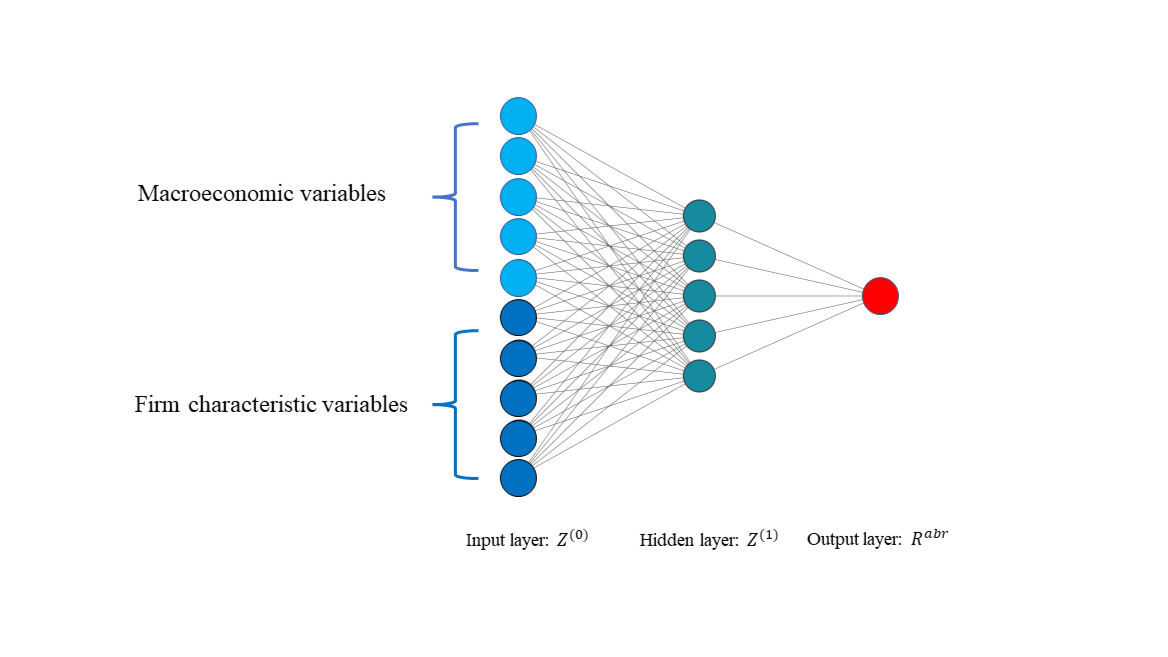
\includegraphics[width=.8\textwidth]{images/fnw_demonstration.png}
  \label{fig: ff-neural network}
\end{figure} 

As posited by \citet*{gu2020empirical}, the stock return can be described using an additive prediction error model as shown below:

\begin{equation}
\label{eqn: generalized model}
R^{abr}_{i,t+1} = E_t(R^{abr}_{i,t+1}) + \epsilon_{i,t+1}
\end{equation}

Here, $E_t(R^{abr}_{i,t+1}) = g(z;\theta)$, where stocks are indexed as $i=1,2,...,N$ and months are indexed by $t=1,2,...,T$. The function $g(z,\theta)$ denotes a mapping function with a set of predictors $z$ and a set of parameters $\theta$, which correspond to the weights and bias in each layer of the neural network model. Through a feed-forward neural network, the model learns to map the inputs to the outputs by adjusting the weights of each layer in response to the errors the model makes on the training dataset. This can be expressed mathematically as follows:
\begin{equation}
  \label{eqn:update weights}
  g(z;\theta) = \theta_0 + \sum^n_{j=1}x_j\theta_j
  \end{equation}

\subsection{Objective Function}

Due to the high number of unknown parameters, obtaining the perfect weights for a neural network model is impossible. Instead, the objective can be reformulated as an optimization or searching problem, where the algorithm aims to find a set of weights that enables the model to make accurate predictions. The commonly used algorithm for training the neural network model is stochastic gradient descent (SDG), which updates the weights using the backpropagation of errors method. Initially, the model makes predictions using the initial weights, and the error is then calculated based on those predictions. The gradient descent algorithm is then used to adjust the weights so that the prediction error is minimized, see an exhaustive discussion by \citet*{domingos2012few}. Mean squared error (MSE) and mean absolute error (MAE) are common objective functions (i.e. loss functions) used in training the neural network model. However, in our study, since there are significant outliers in the abnormal return data, we followed the convention in empirical asset pricing by choosing MSE as the objective function.

\subsection{Activation Function}

Activation functions are a critical component in neural network construction. The choice of activation function in the hidden layer determines how the weighted sum of inputs is transformed into an output from the previous layer to the next, while the choice of activation function in the final output layer determines the type of prediction the model will make. There are various potential choices for the activation function, such as softmax, sigmoid, and ReLu. The architecture of the neural network model ensures that the interaction effect within different variables is captured, while the proper choice of activation function guarantees that the non-linear impact of individual predictors on expected returns is also taken into account. In this study, a linear function is chosen as the final output activation function because the stock returns being predicted are rather random and contain extreme values. Introduced by \citet*{nair2010rectified}, ReLu is selected as the activation function for each hidden layer due to its simplicity, computing advantages, and following the convention in existing literature. ReLu is a piecewise linear function with two linear pieces that will output the input directly if it is positive; otherwise, it will output zero. It is defined as:

\begin{equation}
  \label{eqn:ReLU}
  ReLU(x) = \begin{cases}
    0 & if \ x < o \\
    x & otherwise,
  \end{cases}
  \end{equation}

\subsection{Learning Rate}

The learning rate is a crucial hyperparameter in neural networks as it governs the magnitude of change to the model during each step of the weight updating process. By controlling the speed of learning, the learning rate is a key factor in determining the performance of the model. When the learning rate is set to a high value, the model is able to learn quickly, but yeild a not so accurate prediction; conversely, a low learning rate can enable the model to reach an optimal, or even globally optimal, set of weights, albeit at the cost of a significantly longer training time. The learning rate typically takes a value in the range of 0 to 1. However, an excessively large learning rate may cause the model's performance to oscillate in each training epoch, resulting in divergent results. Conversely, an overly small learning rate may never converge or become trapped in a suboptimal solution.

To accelerate the model training process and optimize the weight searching procedure, we follow \citet*{smith2017cyclical} and introduce momentum to the learning process and utilize a learning rate schedule. Specifically, we incorporate an exponentially weighted average of prior updates into the next update, allowing previous updates in one direction to continue in that direction in the future. Momentum is independent of the choice of learning rate but can enhance the speed of the optimization process when used in combination with the learning rate, increasing the likelihood of finding an optimal set of weights in fewer training epochs. Instead of utilizing a constant learning rate, we vary the learning rate during the training process, referred to as a learning rate schedule or learning rate decay. The fundamental concept is to employ a larger learning rate at the outset to expedite the training process, and gradually reduce the learning rate as the training epochs progress. This approach avoids oscillating model performance and becoming trapped in suboptimal solutions, or failing to converge entirely. A commonly used formula for the learning rate schedule is shown in Equation \ref{eqn:learningrate}:

\begin{equation}
  \label{eqn:learningrate}
  Learning \ Rate = Initial \ Rate * \frac{1}{1 + decay * iteration}
  \end{equation}

\noindent In comparison with a fixed learning rate, utilizing a learning rate schedule can reduce sensitivity to the initial learning rate and provide improved performance. The selection of the learning rate can be visualized through a plot of the changing pattern, as shown in Figure \ref{fig: learningrate}.

\begin{figure}[H]
  \centering
  \caption{\textbf{Learning Rate Scheduale}}
  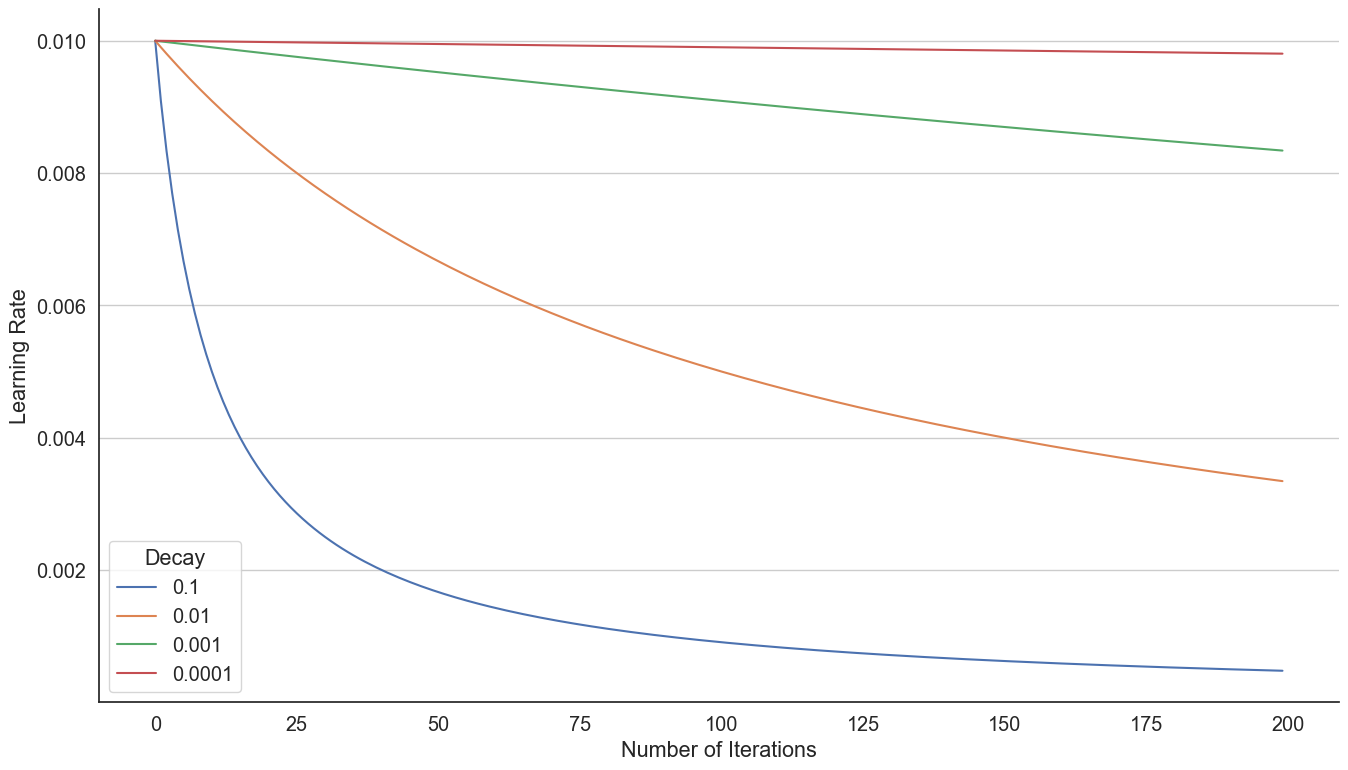
\includegraphics[width=.8\textwidth]{images/learning rate decay.png}
  \label{fig: learningrate}
  \caption*{\footnotesize{This graphic shows a basic learning rate schedule with different decay rates.  The initial learning rate is 0.01, and along with the increasing number of iterations the learning rate starts to decrease to achieve a state of art accuracy.}}
\end{figure}

\subsection{Fix Overfitting with Regularization}

Overfitting is one of the most significant challenges associated with neural network models, where the model performs exceptionally well on the training data but poorly on the test data. The objective of machine learning is to enable the model to learn from example data and generalize to explain new data in the future; however, an overfitted model cannot accomplish this goal. Various regularization techniques discussed by \citet*{tian2022comprehensive}, including activity regularization, weight constraints, dropout, and noise addition, can be employed to combat overfitting. Of these methods, weight regularization is the most widely used. When a model is fitted with sufficient epochs, the weights can become highly specialized to the training data and lead to overfitting. The weights increase in magnitude to capture the specifics of the training data, but this can cause instability in the model and poor performance in predicting test data due to minor variations. Weight regularization imposes a penalty on the model during training based on the magnitude of the weights, with the objective of keeping the weights small. In this paper, we apply an $L1$ penalty (Lasso) to the network weights to promote sparsity.

\subsection{Improve Prediction with Ensembles}

Neural networks can be highly sensitive to the initial conditions, including the random weights and the specific characteristics of the training data. As a result, different initial conditions can lead to the discovery of different sets of weights, and the model can make different predictions when fed with new input data. To address this issue, a common approach is to train multiple models and combine their predictions to ensure a more stable and accurate final prediction. While combining different models can introduce some bias, it can also alleviate the high variance problem caused by a single model. This approach is commonly referred as ensembled learning. There are multiple ensemble learing methods discussed by \citet*{sagi2018ensemble}, among which we use the simplest method to aggregate 10 neural network models to get robust results.

\subsection{Other Model Settings}

The batch size plays a crucial role in training neural network models, impacting both the prediction accuracy and computational efficiency. It represents the number of training samples used per iteration in the training process. A larger batch size leads to a more accurate estimation as more training samples are used, increasing the likelihood of navigating the weight search towards optimal performance. However, smaller batch sizes can result in noisy weight updates, leading to more robust models in some cases. Therefore, the choice of batch size can affect the accuracy of the estimation, the stability of the learning process, and the speed at which the model learns. Consequently, selecting an appropriate batch size is a trade-off between these factors. As a result, the batch size is a critical hyperparameter in the learning algorithm that requires tuning to optimize the model's performance. \citet*{ioffe2015batch} apply batch normalization method to normalizes the activations of each layer in the network over the mini-batch of samples. They show that Batch Normalization can significantly accelerate the training of deep neural networks by reducing the internal covariate shift problem.

In the context of neural networks, the initialized weights of a model are typically small random variables that are updated during the training process using an optimization algorithm. To generate the initial weights, the He initializer proposed by \citet*{he2015delving} is commonly used. In addition to the initialization of weights, the scale of input and output variables can also have a significant impact on the training process and the resulting model performance. To address this, we used a standardized scaler on the training dataset, which was then applied to both the validation and test datasets. This approach helped to speed up and stabilize the training process, and ensured that the model was able to learn effectively from the available data.

\subsection{Feature Importance}
\label{subsec:feature importance}

While deep learning models have powerful predicting ability, there are still criticisms that claim that methods such as neural networks lack interpretability, and that the models used are more like a "black box". Therefore, correctly interpreting the predicted output is equally as important as the predicting accuracy, as it can provide insights into how the output is influenced by variables, give insights into how a model can be improved, and help understand how the process is being modeled. In this paper, we use SHAP values, as described by \citet*{NIPS2017_8a20a862}, to measure feature importance. SHAP (SHapley Additive exPlanation) values track the change in the predicted outputs made by the model by conditioning on each specific feature. They use additive feature attribution methods, with the following mathematical expression, but replace $f(x)$ with $f_x(z')=f(h_x(z'))=E[f(z)|z_s]$:

\begin{equation}
  \label{eqn:shap}
  f(x)=g(x')=\phi_0+\sum^M_{i=1}\phi_i x'_i
  \end{equation}

The explanation model $g(x')$ is designed to match the original model $f(x)$, where $x = h_x(x')$. In this framework, $\phi_0 = f(h_x(0))$ represents the model output with all simplified inputs dropped off (i.e., missing). The $s$ in $E[f(z)|z_s]$ refers to the set of non-zero indexes in $z'$. If an observation has an actual output value of 0 (the base value), some features may push the predicted output away from the actual value, while other features may pull it back closer to the actual value. The final predicted output $f(x)$ can be seen as the balance of power, as illustrated in Figure \ref{fig: shap_demo}. The SHAP values track the change in the predicted output made by the model conditioning on each specific feature and use an additive feature attribution method, as expressed in the mathematical formula provided earlier in Equation \ref{eqn:shap}.

\begin{figure}[H]
  \centering
  \caption{\textbf{SHAP Value Demonstration}}
  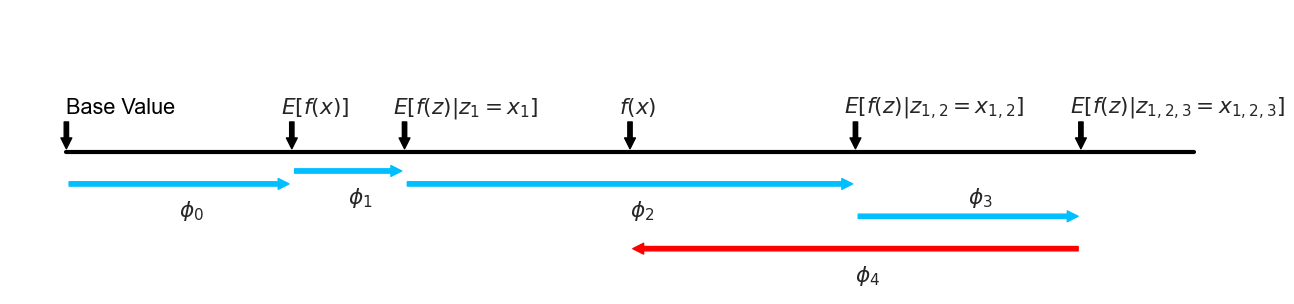
\includegraphics[width=.9\textwidth]{images/shap_force_dem.png}
  \label{fig: shap_demo}
\end{figure}



%%%%%%%%%%%%%%%%%%%%%%%%%%%%%%%%%%%%%%%%%%%%%%%%%%%%%%%%%%%%%%%%
%%%%%%%%%%%%%%%%%%%%%%%%%%%%%%%%%%%%%%%%%%%%%%%%%%%%%%%%%%%%%%%%
\section{Data} \label{sec:data}
\subsection{Firm Characteristics Data}

In this paper, we deviate from the traditional approach of constructing all variables from raw data obtained from databases like Compustat or Thomson Reuters. Instead, we utilize firm characteristic data from Open Source Asset Pricing\footnote{The dataset consists of 319 characteristics that are based on previous asset pricing studies. Out of these, 161 characteristics exhibit significant t-statistics when compared to the original papers, while 44 show mixed evidence and the remaining 114 are found to be insignificant. From the 161 variables that show significant t-statistics, we select our firm characteristic variables based on variable importance discussed in the existing literature while also considering data completeness, in order to minimize the number of missing values in the dataset. The database is maintained and updated annually by the authors, and open-source code is provided for the purpose of enhancing the reproducibility.}, a dataset created and maintained by \citet*{chen2021open}. There are several reasons for this decision. First, machine learning papers typically involve analyzing a large number of feature variables, which can be time-consuming to construct. For instance, \citet*{kozak2020shrinking} used 50 anomaly characteristics and 80 financial ratios from WRDS, while \citet*{freyberger2020dissecting} used 62 characteristics. Second, constructing these feature variables based on the original paper's descriptions requires a meticulous approach, and even small subjective variations can lead to different datasets. Third, using a self-constructed dataset can make reproducing the paper more challenging and reduce comparability with other machine learning papers.

We do not corperate all the variables from the dataset in our analysis, instead only part of variables are selected for the study.The selection of firm characteristic variables for our empirical research is guided by the existing literature on the variables' relevance in predicting stock return, as well as by the completeness of each variable in avoiding the inclusion of too many missing values, which is related with our approach of handling missing values, thereby ensuring a maximally sized dataset. \citet*{gu2020empirical}, \citet*{leippold2022machine}, and \citet*{drobetz2021empirical} replace all missing values with the cross-sectional median of each firm characteristic variables in that month. Although, This approach allow us to include as many firm characteristic variables as we want, it needs strong assumptions on the structure of the data and creates artificial time-series fuctuation in the firm characteristics variables. Given the non-random nature of missing data in firm characteristics, as noted by \citet*{bryzgalova2022missing}, we choose not to use artificial imputation methods, instead opting to drop all missing values to obtain a balanced dataset. In such a way to aviod additional source of errors and keep the dependency structure in the dataset. Our final selection includes 49 firm characteristic variables categorized into 7 categories, namely "Value", "Investment", "Trading", "Profitability", "Momentum", "Intangible", and "Risk", which are similar to those used by \citet*{chen2019deep} as presented in Table \ref{table: Firm Characteristics by Category}. Notably, the Open Source Asset Pricing database does not provide the variables "short-term reversal", "size", and "return", which we abtain from the Center for Research in Security Prices (CRSP) and merge using the unique stock identifier PERMNO and date.

\begin{table}[H]
  \footnotesize
  \centering
  \caption{Firm Characteristics by Category}
  \label{table: Firm Characteristics by Category}
  \begin{tabularx}{\linewidth}{ ll >{\setlength\hsize{11\hsize}} X ll>{\setlength\hsize{11\hsize}} X}
  \cline{1-6}
  ~ & \textbf{Value} & ~ & ~ & \textbf{Moment} \\\cline{2-3} \cline{5-6}
  1 & AssetGrowth & Asset growth & 27 & LRreversal & Long‐run reversal \\
  2 & Size & Size & 28 & STreversal & Short term reversal \\
  3 & SP & Sales‐to‐price & 29 & Mom12m & Momentum (12 month) \\
  4 & NOA & Net Operating Assets & 30 & Mom6m & Momentum (6 month) \\
  5 & AM & Total assets to market & 31 & MRreversal & Medium‐run reversal \\
  6 & ChEQ & Growth in book equity & 32 & IntMom & Intermediate Momentum \\
  7 & DelEqu & Change in equity to assets & 33 & ResidualMomentum & Momentum based on FF3 residuals \\
  8 & ChNWC & Change in Net Working Capital & ~ & ~ & ~ \\
  9 & BMdec & Book to market using December ME & ~ & ~ & ~ \\
  ~ & ~ & ~ & ~ & \textbf{Risk} & ~ \\\cline{5-6}
  ~ & \textbf{Investment} & ~ & 34 & CF & Cash flow to market \\\cline{2-3}
  10 & ShareRepurchase & Share repurchases & 35 & IdioRisk & Idiosyncratic risk \\
  11 & ShareIss1Y & Share issuance (1 year) & 36 & Leverage & Market leverage \\
  12 & InvestPPEInv & change in ppe and inv/assets & 37 & BookLeverage & Book leverage (annual) \\
  13 & dNoa & change in net operating assets & 38 & IdioVol3F & Idiosyncratic risk (3 factor) \\
  14 & DelLTI & Change in long‐term investment & 39 & DelFINL & Change in financial liabilities \\
  15 & DelCOA & Change in current operating assets & 40 & cfp & Operating Cash flows to price \\
  16 & GrLTNOA & Growth in long term operating assets & 41 & DelCOL & Change in current operating liabilities \\
  ~ & ~ & ~ & ~ & ~ & ~ \\
  ~ & \textbf{Trading Frictions} & ~ & ~ & \textbf{Profitbility} & ~ \\\cline{2-3} \cline{5-6}
  17 & Price & Price & 42 & CashProd & Cash Productivity \\
  18 & Beta & CAPM beta & 43 & roaq & Return on assets (qtrly) \\
  19 & High52 & 52 week high & 44 & GP & gross profits / total assets \\
  20 & BidAskSpread & Bid‐ask spread & 45 & RoE & net income / book equity \\
  21 & VolSD & Volume Variance & ~ & ~ & ~ \\
  22 & DolVol & Past trading volume & ~ & \textbf{Intangible} & ~ \\\cline{5-6}
  23 & Illiquidity & Amihud's illiquidity & 46 & Accruals & Accruals \\
  24 & BetaFP & Frazzini‐Pedersen Beta & 47 & OPLeverage & Operating leverage \\
  25 & VolMkt & Volume to market equity & 48 & AbnormalAccruals & Abnormal Accruals \\
  26 & MaxRet & Maximum return over month & 49 & PctAcc & Percent Operating Accruals \\
  \hline
  \end{tabularx}
\end{table}

\subsection{Macroeconomic Data}
\label{sec: macro data}
We choose CFNAI (Chicago Fed National Activity Index) index to proxy the macroeconomic conditions, as it is a commonly used measure of overall macroeconomic conditions in the US. The CFNAI is reported monthly by the Federal Reserve Bank of Chicago and is often used as a leading indicator of economic growth or recession. It is a widely followed measure in both academic and policy circles. The comprehensive CFNAI index is plotted in figure \ref{fig: CFNAI index} and the subsectional macroeconomic indices including Production and income; Employment, unemployment, and hours; Personal consumption and housing; Sales, orders, and inventories which are detailed in Appendix \ref{sec:appendixa} and presented in Figure \ref{fig: Subsectional Macroeconomic index} together with NBER suggested recession indicators.

\begin{figure}[H]
  \centering
  \caption{\textbf{CFNAI index}}
  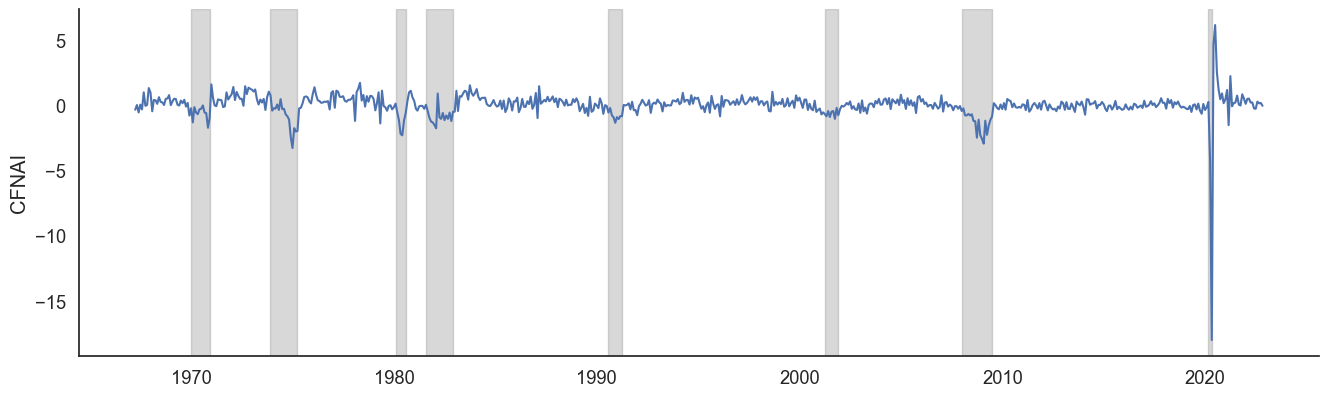
\includegraphics[width=.8\textwidth]{images/cfnai.png}
  \label{fig: CFNAI index}
  \caption*{\footnotesize{This graphic plots the historical CFNAI index from 1965 to 2022 together with NBER suggested recession periods, in 2020 the CFNAI index fell sharply due to the economic impact of the COVID-19 pandemic.}}
\end{figure} 

\subsection{Market Sentiment}
For additional analysis, we also use market sentiment data to capture the overall macroeconomic conditions. \citet*{baker2007investor} find that market sentiment, or the overall attitude of investors towards the market, can have a significant impact on stock returns. To measure market sentiment, they construct a sentiment index based on five indicators covering a wide range of measures of investor sentiment. The historical trend chart of investors sentiment is plotted in figure \ref{fig: sentiment index}, and the 5 components for constructing the investors sentiment index are also plotted in figure \ref{fig: 5 components for sentiment} in Appendix \ref{sec:appendixa2}.

\begin{figure}[H]
  \centering
  \caption{\textbf{Investors Sentiment}}
  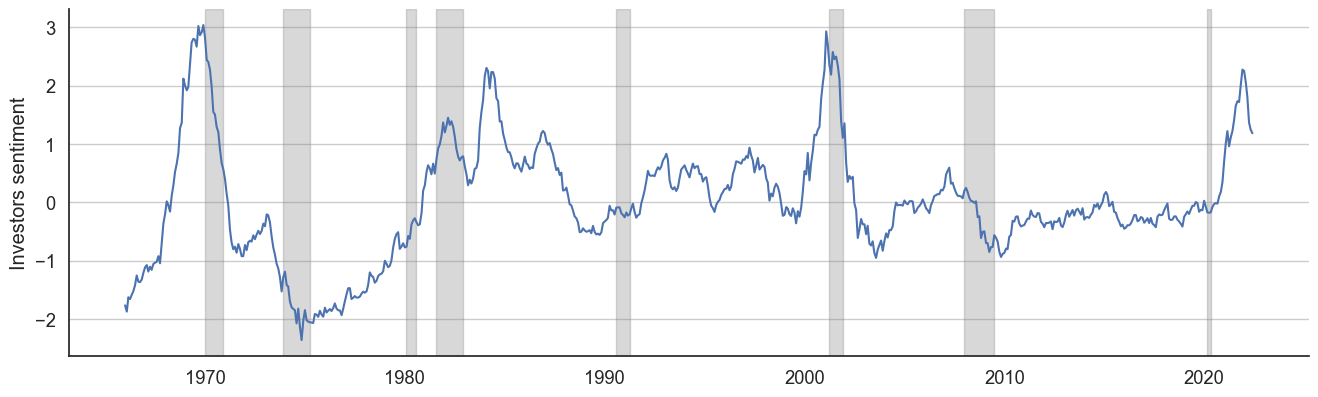
\includegraphics[width=.8\textwidth]{images/sentiment.png}
  \label{fig: sentiment index}
  \caption*{\footnotesize{Data are generally as used and described in the paper \citet*{baker2007investor} and \citet*{baker2006investor}.}}
\end{figure} 

\subsection{Fama-French 5 Factor Data}

In this study, the Fama-French 5 factor dataset and risk-free rate are incorporated from the Fama-French data library and merged with the primary dataset. A summary of the variables can be found in Table \ref{table: Fama-French 5 factor}, while an in-depth discussion on their construction and economic rationale can be found in \citet*{fama2015five} work. The collected data spans from July 1963 to the present, with a monthly frequency.

\begin{table}[H]
  \centering
  \footnotesize
  \caption{\textbf{Fama-French 5 Factor}}
  \label{table: Fama-French 5 factor}
  \begin{tabular}{l>{\RaggedRight}p{0.8\linewidth}}
  \hline
      \textbf{Acronym} & \textbf{Defination} \\ \hline
      SMB & SMB (Small Minus Big) is the average return on the nine small stock portfolios minus the average return on the nine big stock portfolios. \\ 
      HML & HML (High Minus Low) is the average return on the two value portfolios minus the average return on the two growth portfolios. \\ 
      RMW & RMW (Robust Minus Weak) is the average return on the two robust operating profitability portfolios minus the average return on the two weak operating profitability portfolios.  \\ 
      CMA & CMA (Conservative Minus Aggressive) is the average return on the two conservative investment portfolios minus the average return on the two aggressive investment portfolios. \\ 
      Mkt-RF & Rm-Rf, the excess return on the market, value-weight return of all CRSP firms incorporated in the US and listed on the NYSE, AMEX, or NASDAQ that have a CRSP share code of 10 or 11 at the beginning of month t, good shares and price data at the beginning of t, and good return data for t minus the one-month Treasury bill rate (from Ibbotson Associates). \\ 
      RF & One-month Treasury bill rate (from Ibbotson Associates). \\ \hline
  \end{tabular}
  \begin{tablenotes}
    \small
    \item The Fama/French 5 factors (2x3) are constructed using the 6 value-weight portfolios formed on size and book-to-market, the 6 value-weight portfolios formed on size and operating profitability, and the 6 value-weight portfolios formed on size and investment.
  \end{tablenotes}
\end{table}

\subsection{Abnormal Return}

The purpose of this study is to compare the performance of neural network models in predicting different measures of stock return. Specifically, we focus on stock excess return, which is defined as the actual stock return minus the one-month Treasury bill rate, and we construct stock abnormal return using the methodology of \citet*{kaniel2022machine}. To be precise, we define the abnormal return for each stock as the difference between the actual excess return and the expected return based on factor models, i.e., the alpha of the factor models.

Over the years, the field of finance has witnessed significant changes in the prevalence of factor models used for pricing assets. Starting from the classic Capital Asset Pricing Model (CAPM) introduced by \citet*{sharpe1964capital}, the evolution of asset pricing models led to the Intertemporal Capital Asset Pricing Model (ICAPM) by \citet*{merton1973intertemporal}. The Fama-French Three-Factor Model (FF3) proposed by \citet*{fama1992cross} gained popularity for being able to better explain the cross-section of stock returns than the CAPM. However, it has since been replaced by the more recent Fama-French Five-Factor Model (FF5) introduced by the same authors \citet*{fama2015five}. Moreover, researchers have proposed unofficial extensions to the FF5 model, such as the Fama-French Five-Factor Model with Momentum (FF5F+M) and the Fama-French Six-Factor Model (FF6), which includes a volatility factor, as suggested in a paper by \citet*{harvey2016and}. To ensure the study covers the historical trend without drifting too much from the main academic consensus, we aim to compare the abnormal returns obtained using CAPM, FF3, and FF5 models, given the long time horizon of our analysis spanning over five decades.

Specifically, we first require that each stock has at least 37 observations and estimate betas for each of the factors over the past 36 months, using equation \ref{eqn:abnormal return 1} as presented below:

\begin{equation}
  \label{eqn:abnormal return 1}
  R_{i,t-36:t} = \alpha_{i,t-36:t} + F_{t-36:t} \hat{\beta}_{i,t} + \epsilon_{i, t-36:t}
\end{equation}

\noindent in which $R_{i,t}$ is the return of stock $i$ in month $t$ in excess of a one-month risk-free rate, $F_t$ is a vector of factors, take Fama-French 5 factors model as an example, $F_t$ would be $[SMB_t + HML_t + RMW_t + CMA_t + (R_m - R_f)_t]$, and $\hat{\beta}_{i,t}$ is a vector of estimated coefficients accordingly. Then, we use the estimated $\hat{\beta}_{i,t}$ from the past 36 months to predict the stock return for 37th month $R^E_{i,t+1} = F_{t+1}\hat{\beta}_{i,t}$. Finally, the abnormal return for the stock is obtained as the difference between the actual excess return and the Fama-French 5 factors' expected return, using equation \ref{eqn:abnormal return 2}.

\begin{equation}
  \label{eqn:abnormal return 2}
  R^{abn}_{i,t+1} = R_{i,t+1} - R^E_{i,t+1}
\end{equation}

Figure \ref{fig: abnormal_excess_return} presents a graphical representation of the key features of stock excess and abnormal returns. The left panel showcases the cumulative monthly average excess and abnormal returns, together with the shaded NBER suggested recession periods. The cumulative excess return displays a clear upward slope, indicating a considerable increase of over four times high from the first to the last month. And several drawdowns happend during or next to the NBER suggested recession periods. In contrast, the cumulative abnormal returns from the CAPM model oscillate within the range of [0,1], whereas those from the 3- and 5-factor models fluctuate within the range of [-1,0]. Nevertheless, some drawdowns in the cumulative monthly average abnormal returns coincide with the NBER suggested recession periods. Among stock abnormal returns derived from different factor models, the abnormal return generated by the 5-factor model deviates the least from zero line, suggesting that it is the best factor model for predicting stock returns among other factor models.

The right panel of Figure \ref{fig: abnormal_excess_return} displays the monthly standard deviation of stock excess and abnormal returns. Most of the time, the monthly standard deviation of excess and abnormal stock returns overlap with each other. However, there is a peak in abnormal returns from the 5-factor model around 2004 that cannot be explained. We also provide a summary of the statistics for various measurements of stock returns in Appendix Table \ref{table: Summary statistic of return}, as well as a heatmap in Figure \ref{fig: abnormal_excess_corr} illustrating their correlations.

\begin{figure}[H]
  \centering
  \caption{\textbf{Cumulative Excess and Abnormal Return}}
  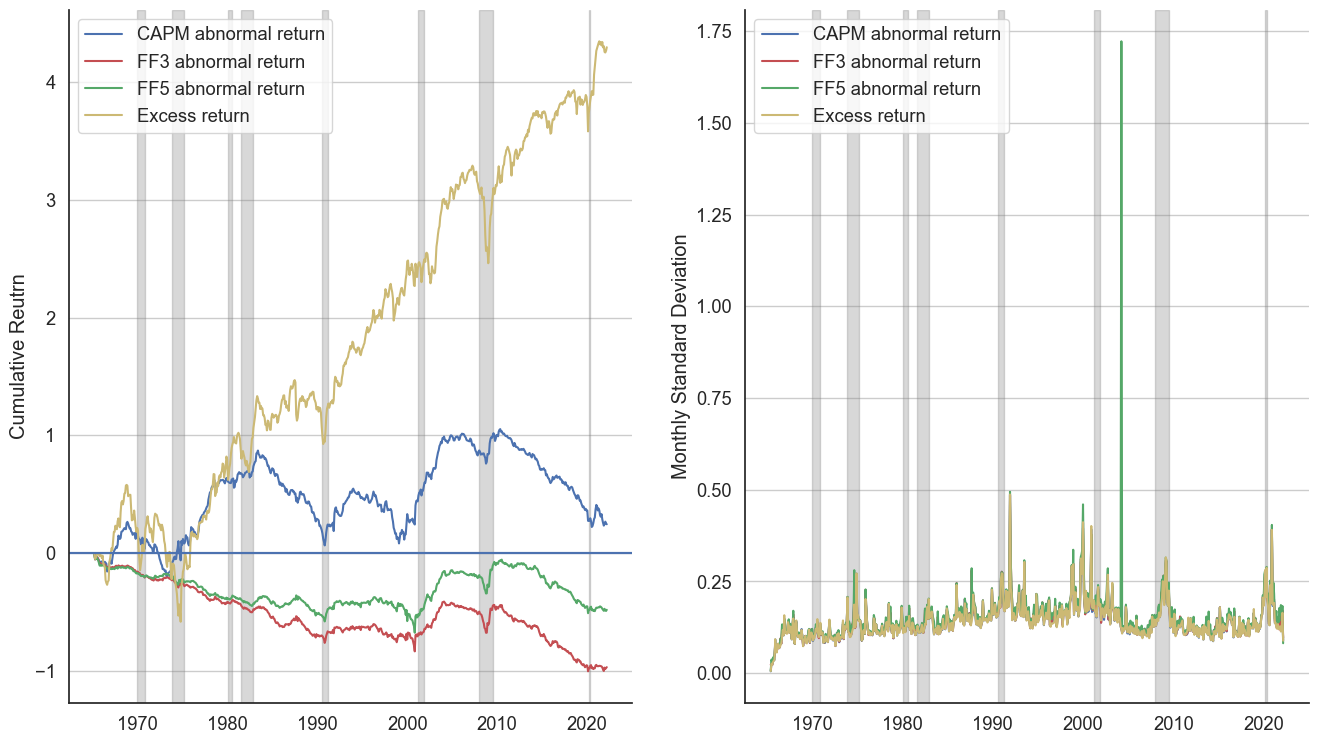
\includegraphics[width=.8\textwidth]{images/abnormal_excess_return.png}
  \label{fig: abnormal_excess_return}
  \caption*{\footnotesize{The left panel of this figure shows the monthly average excess and abnormal return accumulated for the whole time period in our dataset. The left panel presents the standard deviation of stock excess and abnormal returns in each month.}}
\end{figure} 

\subsection{Related to Neural Network}

To ensure that the neural network model is trained on a balanced dataset, it is important to handle missing values carefully. Previous studies such as \citet*{gu2020empirical} and \citet*{gu2019autoencoder} have used the cross-sectional median for each feature variable during the respective month to replace the missing values. However, this approach introduces artificial data and may compromise the dependency structure, resulting in additional errors. To address this issue, we adopt the approach of \citet*{kelly2019characteristics} and \citet*{chen2019deep}, which involves dropping all the missing observations from the dataset. This also explains why we do not include all 161 variables from the database. The resulting dataset for firm characteristics contains more than 10,000 companies with over 1,100,000 observations. The sample period covers stocks from December 1971 to December 2021, spanning a total of 50 years.

One commonly used methodology for sample splitting in studies, as demonstrated in works such as \citet*{kozak2020shrinking}, \citet*{gu2020empirical}, and \citet*{chen2019deep}, is to split the data chronologically. This approach, for example, usually allocating the initial 20 years for the training dataset, the subsequent 10 years for validation, and the final 20 years for testing. However, in this study, we adopt a different approach based on the methodology proposed by \citet*{kaniel2022machine}. We divide the full sample into three subsamples of equal length randomly. The first sample is utilized as the training dataset to estimate the neural network model. The second sample serves as the validation dataset to tune the hyperparameters, such as the depth of the model, number of nodes in each layer, choice of learning rate, and regularization penalties. The final sample is reserved as the test dataset to evaluate the performance of out-of-sample predictions. The random sampling of the dates is predicted  on the assumption that the mapping function between stock returns and the conditioning information variables is independent over time, akin to strict cross-section asset pricing analyses.

The methodology used for sample splitting in our study is crucial for three reasons. Firstly, it enables us to conduct an analysis of the impact of macroeconomic conditions on stock returns. Certain macroeconomic conditions, such as low CFNAI index values during recession periods, are only present in a small subset of the data and may be overlooked in conventional chronological data splitting. Secondly, the performance of the neural network model can be severely impacted if there is any unobserved time trend. By using the random sample splitting methodology, all periods of the data are evenly distributed in the training, validation, and test datasets, allowing the model to learn from data across all time periods even if some important variables are not included in the dataset. This methodology ensures that our model can provide reliable predictions. Lastly, the use of the random sample splitting method allows us to use data from all time periods for the out-of-sample analysis, diminishing the effect of specific subperiods. If we follow the conventional chronological sample splitting methodology, the evaluation would only focus on the shorter last part of the data, potentially ignoring important information from earlier periods.

As discussed in Section \ref{sec:neural network}, we select the mean squared error as our objective function to optimize the weights and the rectified linear unit (ReLU) as the activation function to capture the non-linear transformations from the input to hidden layers. We utilize the 'He initializer' to avoid the problem of "dying ReLU". The maximum number of epochs during each training process was set to 100, and early stopping was implemented based on the R-Squared value in the validation dataset.

To enhance the stability of the training process, we use batch normalization, and to improve the robustness of our predictions, we employe ensembled learning by combining the predictions of 10 models. The detailed model specifications are presented in Table \ref{table: model summary}, and the optimal network architecture comprises one hidden layer with 32 hidden nodes. The other hyperparameters are tuned using the validation dataset and are listed in the left panel of the table.

\begin{table}[H]
  \centering
  \caption{\textbf{Model Summary}}
  \begin{tabular}{lllll}
  \hline
      \multicolumn{3}{c}{Tunning Parameters} & \multicolumn{2}{c}{Other Parameters}\\ \cline{4-5}
      Parameters & Candidates & Final Model & Objective Function & MSE \\ \cline{1-3}
      Hidden Layers  & 1, 2, 3 & 1 & Activation Function  & ReLU \\ 
      Hidden Nodes  & 32 , 16, 4 & 32 & Kernel Initializer & He Initializer \\ 
      Learning Rate & 0.01, 0.001 & 0.01 & Ensembled Models & 10 \\ 
      Decay Rate & 0.01, 0.001 & 0.001 & Maximum Epochs & 100 \\ 
      Momentum & 0.95, 0.99 & 0.99 & Early Stop Monitor  & Validation R2 \\ 
      L1 Weight Penalty & 0.001, 0.005 & 0.005 & Early Stop Patience & 10 \\ 
      Batch Size  & 3200, 32000 & 3200 & Batch Normalization & Applied \\ \hline
  \end{tabular}
  \label{table: model summary}
\end{table}



%%%%%%%%%%%%%%%%%%%%%%%%%%%%%%%%%%%%%%%%%%%%%%%%%%%%%%%%%%%%%%%%
%%%%%%%%%%%%%%%%%%%%%%%%%%%%%%%%%%%%%%%%%%%%%%%%%%%%%%%%%%%%%%%%
\section{Results} \label{sec:result}
\subsection{Univariate Long-short Portfolios' Return}
\label{sec: univariate ls portfolios}
Before the main analysis, we exam the predicting power of our firm characteristic feature variables with regard to stock abnormal returns derived from Fama-Frech 5 factors model. We build univariate long-short portfolios based on each one of the 45 firm characteristic feature variables. There are 4 firm characteristic variables ('ShareIss1Y',  ShareRepurchase', 'DelFINL', 'DelLTI'), which could not be cut into deciles, are excluded. First, we sort the stocks into deciles based on each of the 45 firm characteristic feature variables. Then, we buy those stocks sorted in the top decile and sell those sorted in the bottom deciles. All the firm feature variables are signed to make sure the top decile makes better returns than the bottom deciles on average. Worth to mention that the univariate long-short portfolio stratagy only focus on the predicting power of each specific firm feature variable. The portfolios span all the sample period, it ignors the time-varying trend in the panel data, it does not account any interaction effects among different variables and neglects non-linear relationship between firm features and returns. 

Figure \ref{fig: ff5 univariate ls cumulative return} displays the cumulative abnormal returns of the long-short portfolios derived from the FF5 factors model. The majority of the portfolios exhibit high cumulative returns throughout the entire sample period, particularly the portfolios constructed based on short-term reversal (STreversal), price in 52 weeks high (High52), and Size. On the other hand, we also observe a few portfolios with poor performance, which implies that the corresponding firm characteristic variables lack predictive power for stock returns. It is worth noting that these findings hold across various measurements of stock returns, as demonstrated in Appendix \ref{sec:appendixb1}. However, the predictive power of firm characteristic variables may differ across different measures of stock return\footnote{In the Appendix \ref{sec:appendixb1}, we present the univariate long-short portfolios cumulative returns in different measures of stock returns. The ranking of portfolios' performance might not be exactly the same, but the results are robust. Indicating some firm feature variables have strong predictive power regardless which measures of stock return are used.}.

\begin{figure}[H]
  \centering
  \caption{\textbf{FF5 Abnormal Return: Univariate Long-short Portfolios' Cumulative Return}}
  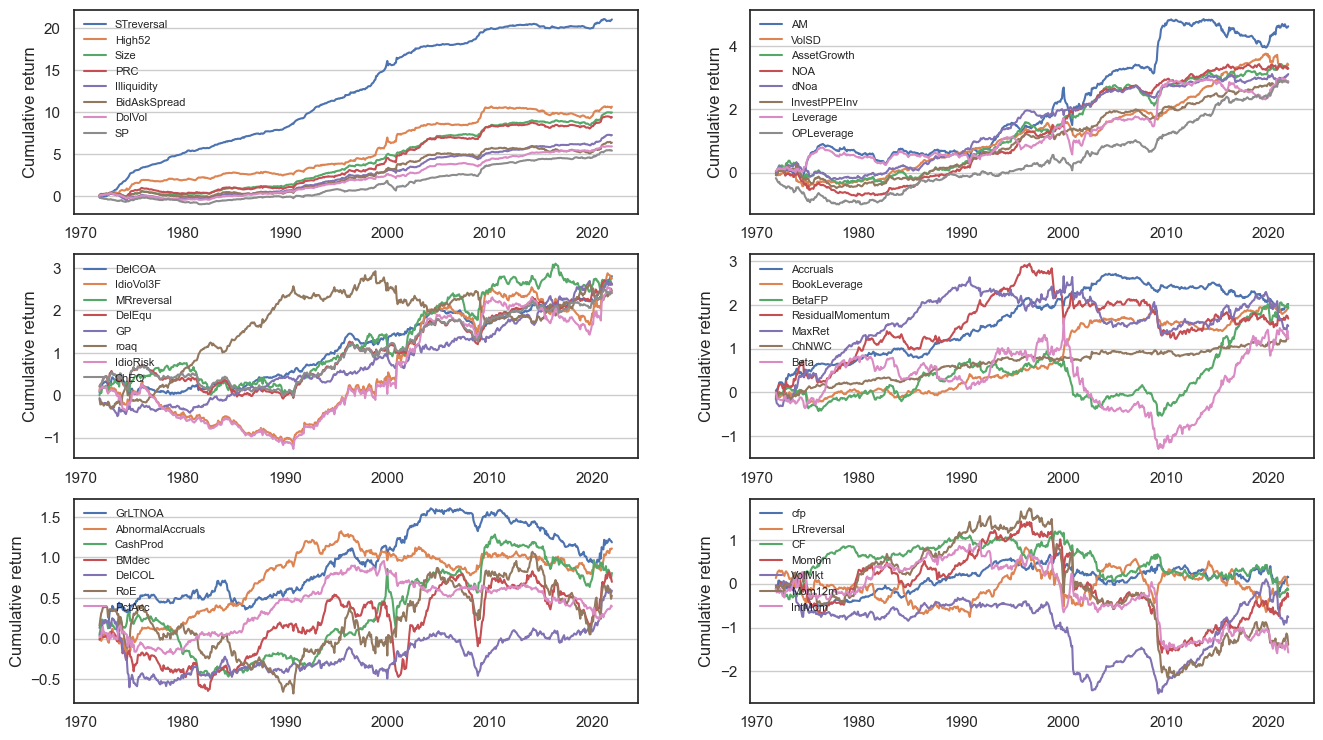
\includegraphics[width=.8\textwidth]{images/univariate_ls_cum_ret_ff5.png}
  \label{fig: ff5 univariate ls cumulative return}
  \caption*{\footnotesize{This graphic showcases firm characteristics sorted univariate long-short portfolios' cumulative return acrossing the whole time period, the return refering to the abnormal return derived from FF5 factor model.}}
\end{figure}

Table \ref{table: ff5 univariate ls portfolio} reports the Sharpe ratio and mean abnormal return of the firm characteristic sorted univariate long-short portfolios with respect to the stock abnormal return derived from the FF5 factors model. For robustness analysis targeting other measures of stock returns, refer to Appendix \ref{sec:appendixb1}. The first two columns present the portfolios' Sharpe ratio and mean abnormal return in the full sample. The majority of long-short portfolios achieve a Sharpe ratio greater than 0.02 and a mean abnormal return exceeding 0.1\% on a monthly average. In comparison with the market performance, the equal weighted portfolio's Sharpe ratio is 0.016 with a mean abnormal return of 0.098\%, while the value-weighted portfolio's Sharpe ratio is 0.01 with a mean return of 0.052\%. These results suggest that most of the firm characteristics possess predictive power for stock abnormal returns, and the formulated long-short portfolios based on those variables outperform the market abnormal return.

\begin{table}[H]
  \centering
  \footnotesize
  \caption{\textbf{FF5 Abnormal Return: Univariate Long-short Portfolios' Returns}}
  \label{table: ff5 univariate ls portfolio}
  \begin{tabular}{lcc|cc|cc|cc}
  \hline
      ~ & \multicolumn{2}{c}{Full Sample} & \multicolumn{2}{c}{Recession} & \multicolumn{2}{c}{Normal} & \multicolumn{2}{c}{Expansion} \\
      ~ & SR & Mean & SR & Mean & SR & Mean & SR & Mean \\ \hline
      STreversal & 0.035 & 0.484 & 0.041 & 0.499 & 0.029 & 0.403 & 0.035 & 0.559 \\
      Size & 0.017 & 0.284 & 0.017 & 0.260 & 0.015 & 0.283 & 0.018 & 0.313 \\ 
      Illiquidity & 0.012 & 0.237 & 0.010 & 0.175 & 0.012 & 0.281 & 0.014 & 0.284 \\ 
      DolVol & 0.010 & 0.224 & 0.008 & 0.164 & 0.010 & 0.245 & 0.012 & 0.280 \\ 
      High52 & 0.018 & 0.215 & 0.024 & 0.249 & 0.011 & 0.136 & 0.017 & 0.257 \\ 
      PRC & 0.016 & 0.213 & 0.022 & 0.253 & 0.010 & 0.158 & 0.014 & 0.216 \\ 
      SP & 0.009 & 0.174 & 0.011 & 0.165 & 0.008 & 0.195 & 0.008 & 0.185 \\ 
      BidAskSpread & 0.011 & 0.164 & 0.013 & 0.175 & 0.006 & 0.103 & 0.013 & 0.203 \\ 
      NOA & 0.005 & 0.159 & 0.010 & 0.255 & 0.002 & 0.070 & 0.004 & 0.120 \\ 
      VolSD & 0.006 & 0.159 & 0.002 & 0.038 & 0.010 & 0.361 & 0.006 & 0.175 \\ 
      dNoa & 0.005 & 0.158 & 0.007 & 0.217 & 0.002 & 0.057 & 0.006 & 0.183 \\ 
      InvestPPEInv & 0.005 & 0.150 & 0.006 & 0.157 & 0.004 & 0.132 & 0.005 & 0.158 \\ 
      DelCOA & 0.005 & 0.144 & 0.005 & 0.146 & 0.001 & 0.028 & 0.008 & 0.229 \\ 
      AssetGrowth & 0.006 & 0.137 & 0.007 & 0.155 & 0.004 & 0.115 & 0.005 & 0.137 \\ 
      AM & 0.008 & 0.134 & 0.011 & 0.144 & 0.003 & 0.067 & 0.009 & 0.195 \\ 
      OPLeverage & 0.005 & 0.127 & 0.007 & 0.179 & 0.005 & 0.170 & 0.002 & 0.040 \\ 
      Accruals & 0.003 & 0.118 & 0.005 & 0.162 & 0.000 & -0.006 & 0.005 & 0.172 \\ 
      GP & 0.004 & 0.115 & 0.003 & 0.078 & 0.008 & 0.213 & 0.002 & 0.063 \\ 
      BookLeverage & 0.003 & 0.112 & 0.002 & 0.064 & 0.007 & 0.289 & 0.001 & 0.042 \\ 
      DelEqu & 0.004 & 0.104 & 0.008 & 0.171 & 0.001 & 0.015 & 0.004 & 0.105 \\ 
      ChEQ & 0.004 & 0.100 & 0.008 & 0.166 & -0.001 & -0.031 & 0.005 & 0.128 \\ 
      Leverage & 0.005 & 0.093 & 0.007 & 0.095 & 0.000 & 0.012 & 0.007 & 0.180 \\ 
      ChNWC & 0.002 & 0.092 & 0.004 & 0.185 & 0.000 & 0.013 & 0.001 & 0.060 \\ 
      roaq & 0.004 & 0.083 & -0.001 & -0.023 & 0.011 & 0.223 & 0.004 & 0.084 \\ 
      MRreversal & 0.004 & 0.080 & 0.007 & 0.116 & 0.000 & 0.002 & 0.005 & 0.114 \\ 
      AbnormalAccruals & 0.002 & 0.074 & 0.005 & 0.166 & -0.002 & -0.104 & 0.003 & 0.110 \\ 
      GrLTNOA & 0.002 & 0.073 & 0.002 & 0.096 & -0.001 & -0.037 & 0.004 & 0.140 \\ 
      IdioVol3F & 0.005 & 0.072 & 0.008 & 0.105 & 0.001 & 0.017 & 0.004 & 0.079 \\ 
      BetaFP & 0.003 & 0.069 & -0.003 & -0.049 & 0.009 & 0.230 & 0.004 & 0.112 \\ 
      IdioRisk & 0.004 & 0.065 & 0.008 & 0.107 & 0.000 & 0.003 & 0.004 & 0.065 \\ 
      ResidualMomentum & 0.003 & 0.051 & 0.002 & 0.030 & 0.001 & 0.017 & 0.006 & 0.104 \\ 
      MaxRet & 0.003 & 0.045 & 0.000 & 0.006 & 0.005 & 0.091 & 0.003 & 0.055 \\ 
      CashProd & 0.001 & 0.039 & 0.000 & -0.011 & 0.000 & 0.008 & 0.004 & 0.145 \\ 
      DelCOL & 0.001 & 0.034 & 0.000 & 0.006 & 0.000 & 0.004 & 0.003 & 0.091 \\ 
      BMdec & 0.001 & 0.029 & -0.004 & -0.082 & 0.001 & 0.018 & 0.007 & 0.198 \\ 
      Beta & 0.002 & 0.029 & -0.002 & -0.031 & 0.010 & 0.139 & 0.000 & -0.004 \\ 
      PctAcc & 0.001 & 0.027 & 0.000 & 0.003 & -0.001 & -0.041 & 0.002 & 0.098 \\ 
      RoE & 0.001 & 0.017 & 0.007 & 0.127 & -0.005 & -0.107 & 0.000 & 0.000 \\ 
      cfp & 0.000 & 0.006 & -0.002 & -0.052 & 0.002 & 0.050 & 0.002 & 0.038 \\ 
      LRreversal & 0.000 & -0.001 & 0.006 & 0.100 & -0.007 & -0.111 & -0.001 & -0.009 \\ 
      CF & 0.000 & -0.005 & -0.004 & -0.074 & 0.002 & 0.061 & 0.001 & 0.022 \\ 
      Mom6m & 0.000 & -0.007 & -0.002 & -0.029 & 0.001 & 0.015 & 0.000 & 0.001 \\ 
      VolMkt & -0.001 & -0.023 & -0.008 & -0.118 & 0.005 & 0.117 & 0.000 & 0.009 \\ 
      Mom12m & -0.002 & -0.030 & -0.008 & -0.086 & 0.003 & 0.043 & -0.002 & -0.025 \\ 
      IntMom & -0.003 & -0.041 & -0.007 & -0.090 & 0.001 & 0.022 & -0.002 & -0.037 \\ \hline
  \end{tabular}
  \begin{tablenotes}
    \footnotesize
    \item This table presents firm characteristics sorted univariate long-short portfolios' sharpe ratios and mean returns. The dataset has futher splitted into three different subsamples based on macroeconomic condition indicator -- CFNAI index, named by recession, normal, and expansion period. The return in this table refering to the abnormal stock return derived from FF5 factors model.
  \end{tablenotes}
\end{table}

Next, we study the performance of univariate long-short portfolios in different macroeconomic conditions. The construction of CFNAI index indicating that a positive index reading corresponds to growth above trend and a negative index reading corresponds to growth below trend. Based on CFNAI we sort the data into tertiles, and define those tertiles from top to bottom as expansion, normal, and recession period. In Table \ref{table: ff5 univariate ls portfolio}, columns 3-8 report univariate long-short portfolios' Sharpe ratios and mean abnormal returns across different macroeconomic conditions. The result of comparing those figures horizontally across 3 macroeconomic senarios as presented in Figure \ref{fig: ff5 univariate ls comparing}. 

The left panel of the figure presents the portfolios' Sharpe ratio under different macroeconomic conditions. The frequency of recession and expansion periods ranked in the 1st and 2nd places is higher than that in the 3rd place, indicating that during both recession and expansion periods, the portfolios tend to have higher Sharpe ratios than in normal periods. We observe a similar pattern in the right panel when considering the portfolios' mean return. Based on these results, we can preliminarily conclude that during recession and expansion periods, the Fama-French 5 factor model's predicted return deviates the most from the actual realized stock return, while in normal periods, when the market is less volatile, the model's predicted return deviates the least. Evidently, there exists an interaction effect between stock abnormal return and macroeconomic conditions.

\begin{figure}[H]
  \centering
  \caption{\textbf{FF5 Abnormal Return: Univariate Long-short Portfolios Performance in Different Macroeconomic Conditions}}
  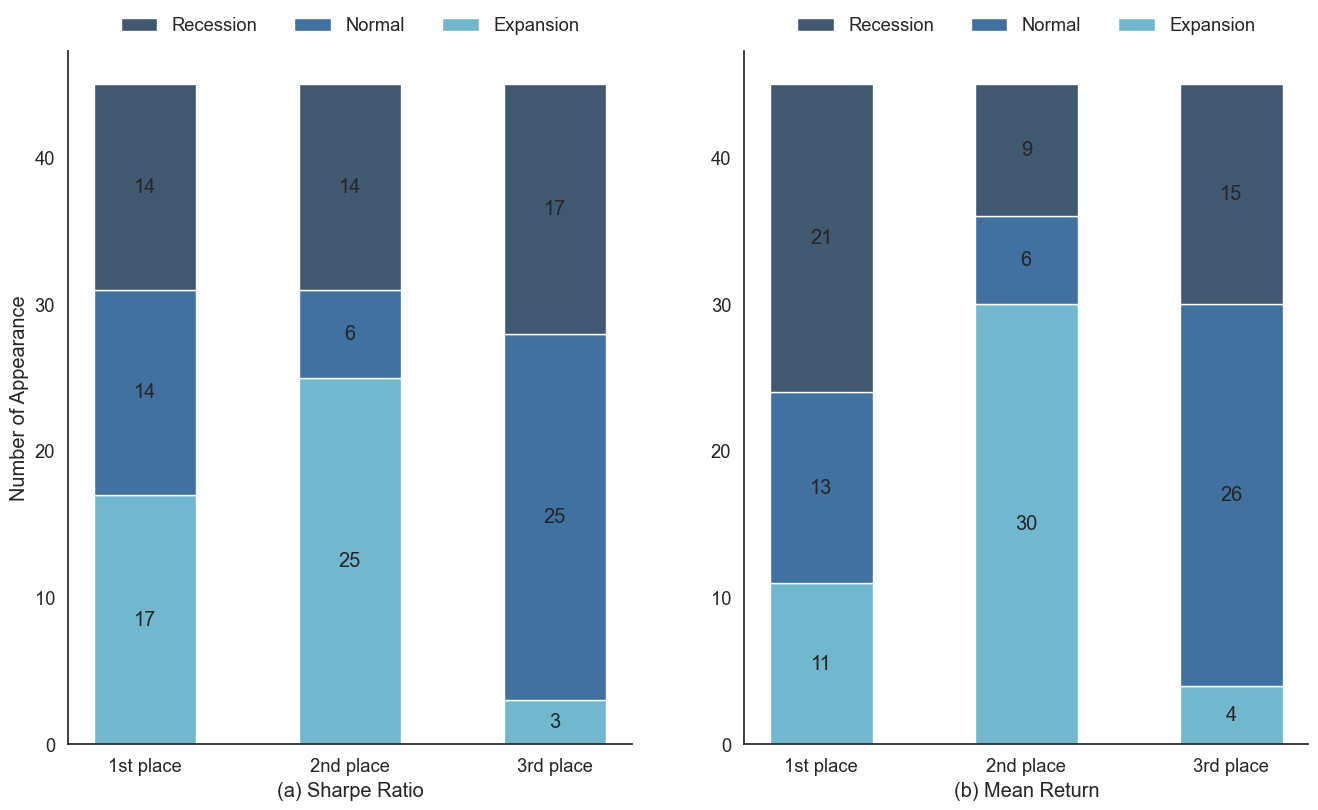
\includegraphics[width=.8\textwidth]{images/univariant_ls_ff5_comparing.png}
  \label{fig: ff5 univariate ls comparing}
  \caption*{\footnotesize{This graphic showcases firm characteristics sorted long-short univariate portfolios' performance across different macroeconomic conditions. We compare univariate long-short portfolios' sharpe ratio and mean return in recession, normal, and expansion periods, which is the horizontal comparision among the last 6 columns in table \ref{table: ff5 univariate ls portfolio}.}}
\end{figure}
\subsection{Analysis with Neural Network Model}

%%%%%%%%%%%%%%%%%%%%%%%%%%%%%%%%%%%%%%%%%%%%%%%%%%%%%%%%%%%%%%%%%%%%%
\subsubsection{Predicting Performance}
Using 49 firm characteristic feature variables listed in table \ref{table: Firm Characteristics by Category}, firstly, we fit the neural network model with the training dataset. Then, we carefully tune the model to get the optimal prediction in the validation dataset. The finalized hyperparameters and model settings are listed in Table \ref{table: model summary}. Then we use the fitted model to predict the next month stock returns in the testing dataset, and to make sure all the predictions are out of sample. We do the same thing by using different measures of stock returns for comparision and report the R-squared value in the testing dataset in Table \ref{table: full sample r2}. The first row of the table reports the R-squared value in the testing dataset by using 49 firm characteristic feature variables sololy. The model's performance does not exhibit significant variation across the different measures of stock returns, as the R-squared values in predicting different targets remain in the vicinity of 0.8\%. Among all the different measures of stock returns, CAPM abnormal return is predicted the most accurately by the model with 0.923\% R-squared value in the testing dataset, while FF3 abnormal returns predicted least accurately with R-squared value 0.763\% in the testing dataset.

As proved by large literatures such as \citet*{cochrane2005financial}, \citet*{welch2008comprehensive}, as well as what we have explored in section \ref{sec: univariate ls portfolios} before, there are some interaction effects between firm characteristic feature variables and macroeconomic conditions for predicting stock return. Hence, we add CFNAI index and investors sentiment data as describled in section \ref{sec: macro data} (since they can be potential indicators that can proxy macroeconomic conditions.) together with the 49 firm features for predicting. In table \ref{table: full sample r2}, the last 3 rows report the R-squared value by using firm characteristic data, CFNAI index data and investors sentiment data combined. Comparing the effectiveness of adding the CFNAI index and investor sentiment data in predicting stock returns, it is observed that the R-squared value increased significantly across various measures of stock returns, especially for adding investors' sentiment data. Furthermore, the model's performance improved the most when combining all feature variables (CFNAI data and investors' sentiment data together), irrespective of the measure of stock returns used. This suggests that both the CFNAI index and investor sentiment data are reliable proxies for capturing macroeconomic conditions when predicting stock returns, and must be considered when conducting such predictions.

Comparing the performance of the neural model across different measures of stock returns after adding CFNAI index and investor sentiment data revealed interesting findings. While the addition of these macroeconomic variables resulted in only a slight increase in the R-squared value in the testing dataset for predicting abnormal returns regardless of which factor models the abnormal returns derived from, however, it has a much greater impact on predicting stock excess returns, as reflected in the substantial increase in the R-squared value in the testing dataset from 0.811\% with only firm characteristic features to 4.005\% with firm characteristic features and all the macroeconomic condition indicators. Therefore, it can be inferred that macroeconomic data is highly beneficial for predicting excess returns, but its significance is not as pronounced when predicting abnormal returns. 

\begin{table}[!ht]
  \centering
  \caption{\textbf{Full Sample R-squared Value in Testing Dataset}}
  \label{table: full sample r2}
  \begin{tabular}{lcccc}
  \hline
  Features & CAPM & FF3 & FF5 & Excess \\ \hline
  Firm & 0.923 & 0.763 & 0.773 & 0.811 \\ 
  Firm + CFNAI & 0.966 & 0.816 & 0.821 & 1.458 \\ 
  Firm + SENT & 1.263 & 0.938 & 0.978 & 2.651 \\ 
  Firm + CFNAI + SENT & 1.396 & 1.011 & 0.998 & 4.005 \\ \hline
  \end{tabular}
  \begin{tablenotes}
    \footnotesize
    \item This table reports R-squared value for predicting stock abnormal reutrn and excess return in the testing dataset, with macroeconomic variables CFNAI index and investor sentiment index.
  \end{tablenotes}
\end{table}

%%%%%%%%%%%%%%%%%%%%%%%%%%%%%%%%%%%%%%%%%%%%%%%%%%%%%%%%%%%%%%%%%%%%%
\subsubsection{Neural Network Portfolios}

Next we build value weighted portfolios based on model's predictions. Each month we sort the stocks into deciles based on their predicted returns, in each decile we assign weights to each component stocks based on their market capitalization. It is important to note that this portfolio formulation process involves rebalancing the portfolios every month and does not consider transaction costs. Figure \ref{fig: portfolios cum return firm features} illustrates the portfolios' cumulative returns (We plot stock abnormal return derived from CAPM, FF3, FF5 models, and stock excess returns all together.) throughout the whole sample period, using only firm characteristic variables for the prediction\footnote{The results of the rest with different conbinations of predictors are listed in the Appendix \ref{sec:appendixb2}.}. The prediction based portfolios can be differentiated from good to bad regardless of which kind of measures used for sotck returns, by following this investing stratagy, we could achieve around 7 times cumulative abnormal returns across the sample period while avoiding potential losses at the same level. The portfolio spectrum is almost symmetrically allocated on both sides of the zero line for stock abnormal returns. In the panel (d) of this figure depicts the cumulative value weighted portfolios based on prediction for stock excess return. Different from abnormal returns, most of the portfolios present upward slops across time instead of nearly symmetrically distributed on the both sides on zero line. And the model can still differentiate between good and bad returns, investing in the top decile can achieve nearly 12 times excess return while investing in the bottom decile would result in a negative return across the whole sample period.

\begin{figure}[H]
  \centering
  \caption{\textbf{Cumulative Return of Portfolios Based on Prediction with Only Firm Features}}
  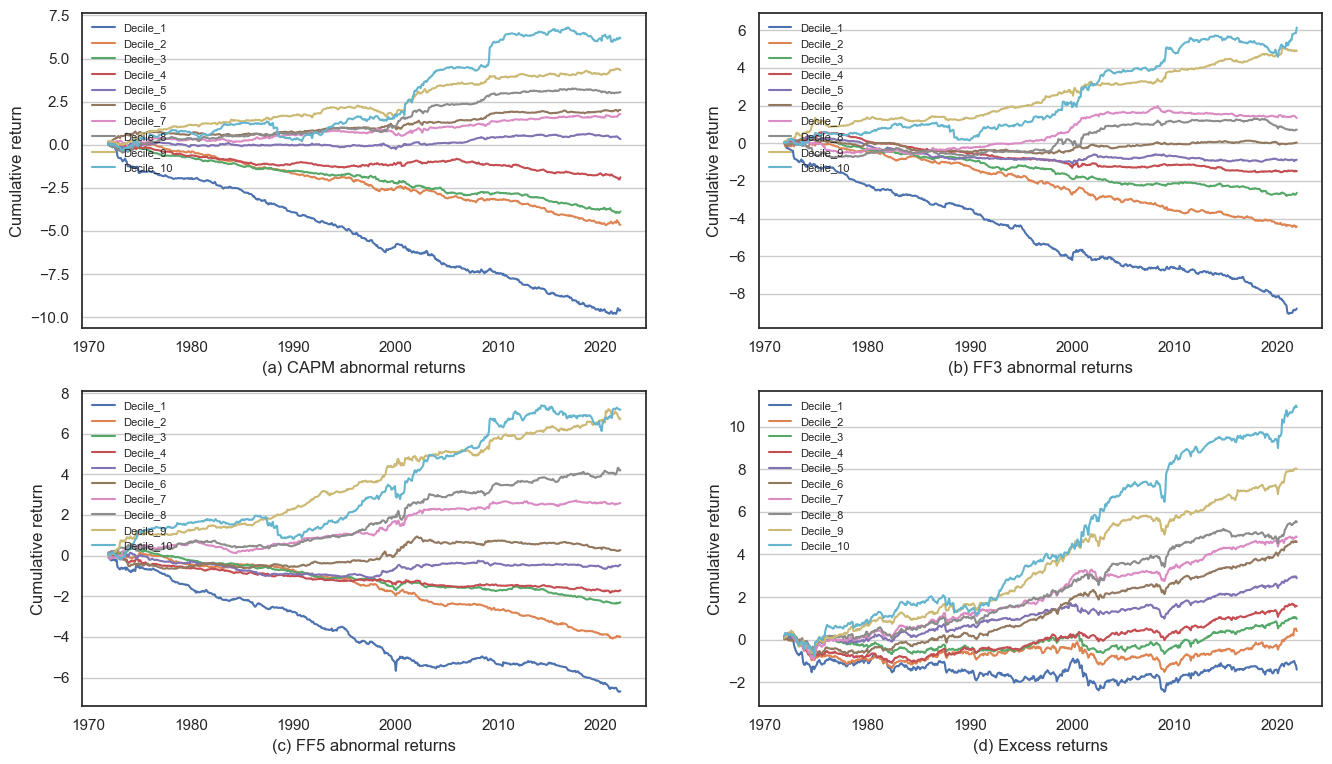
\includegraphics[width=.8\textwidth]{images/vw_portfolios_cumulative_return_firm.png}
  \label{fig: portfolios cum return firm features}
  \caption*{\footnotesize{This graphic shows the cumulative return of value weighted portfolios based on predictions with only firm characteristic feature variables.}}
\end{figure}

We employ the same strategy to formulate value-weighted portfolios based on predictions adding all macroeconomic variables, and explore the cumulative returns as depicted in Figure \ref{fig: portfolios cum return all features}. As we have explored before, the R-squared value in the testing dataset listed in Table \ref{table: full sample r2} is the highest when predicting with firm characteristic features and all macroeconomic variables together, which also indicating the greatest predicitng accuracy. The comparision between cumulative returns of value-weighted portfolios based on all variables and portfolios based solely on firm features supports the findings we have stated before. The top decile in each of the various measures of stock returns exhibits greater differentiation from the other deciles. Furthermore, there are slight improvements in distinguishing between the performance of other portfolios.

\begin{figure}[H]
  \centering
  \caption{\textbf{Cumulative Return of Portfolios Based on Prediction with All Features}}
  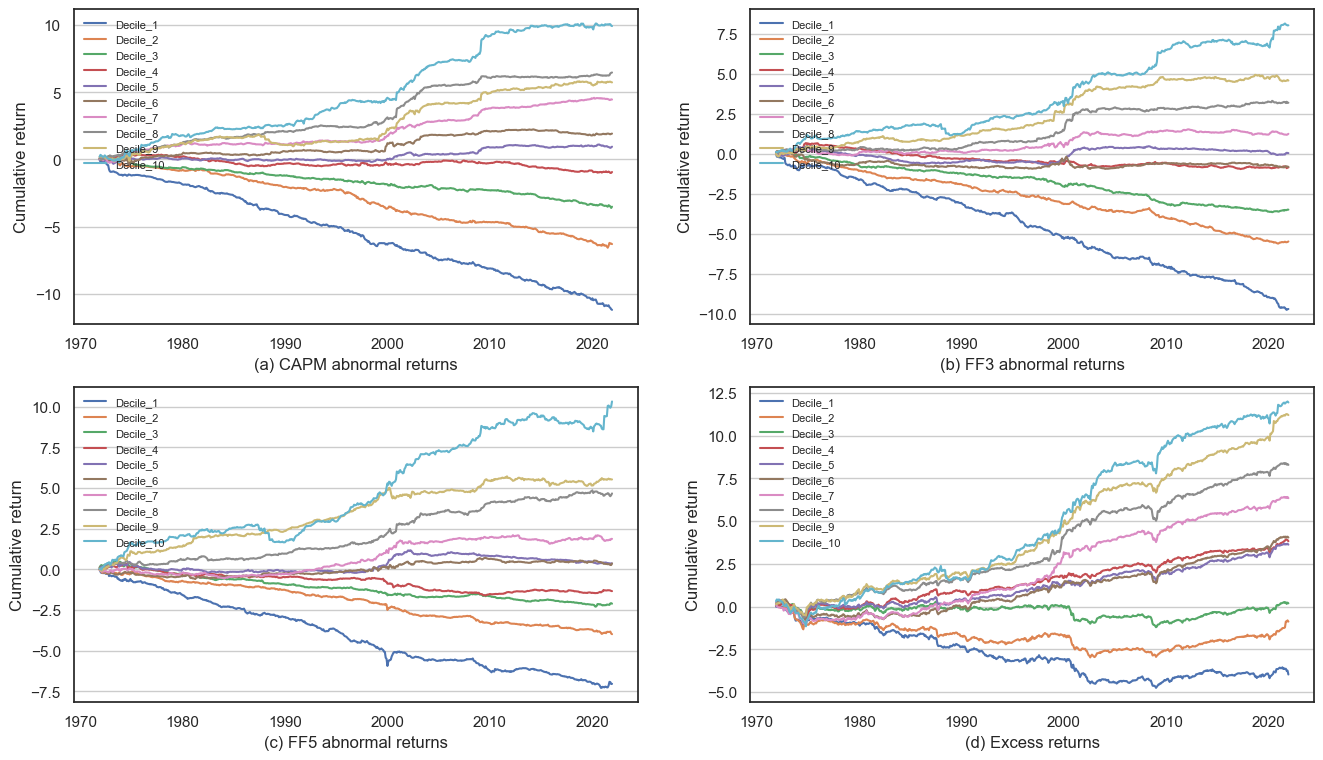
\includegraphics[width=.8\textwidth]{images/vw_portfolios_cumulative_return_all.png}
  \label{fig: portfolios cum return all features}
  \caption*{\footnotesize{This graphic shows the cumulative return of value weighted portfolios based on predictions with only firm characteristic and macroeconomic feature variables.}}
\end{figure}

%%%%%%%%%%%%%%%%%%%%%%%%%%%%%%%%%%%%%%%%%%%%%%%%%%%%%%%%%%%%%%%%%%%%
\subsubsection{Long-short Portfolios Based on Prediction}

In order to compare the performance of long-short portfolios based on model prediction with those based on univariate analysis, we first sort model predicted returns into deciles, then we select the top decile to long and the bottom decile to short, thereby constructing equally-weighted long-short portfolios. We plot the long-short portfolios' cumulative returns for various measures with different information sets in Figure \ref{fig: ls portfolios based on prediction}. The cumulative abnormal returns can exceed more than 25 times for portfolios formulated on prediction with both firm features and macroeconomic data. It is worth noting that in Figure \ref{fig: ff5 univariate ls cumulative return}, the best performance of univariate long-short portfolio based on short-term reversal only has achieved 20 times abnormal returns, and the majority of other univariate long-short portfolios did not generate cumulative abnormal returns of more than 10 times. When examining each panel in Figure \ref{fig: ls portfolios based on prediction}, we observe that the red line, representing the prediction-based long-short portfolios with both firm features and all macroeconomic data, dominates most of the other portfolios based on predictions with firm features alone or with a lack of CFNAI or sentiment data.

\begin{figure}[H]
  \centering
  \caption{\textbf{Cumulative Return of Long-short Portfolios Based on Prediction}}
  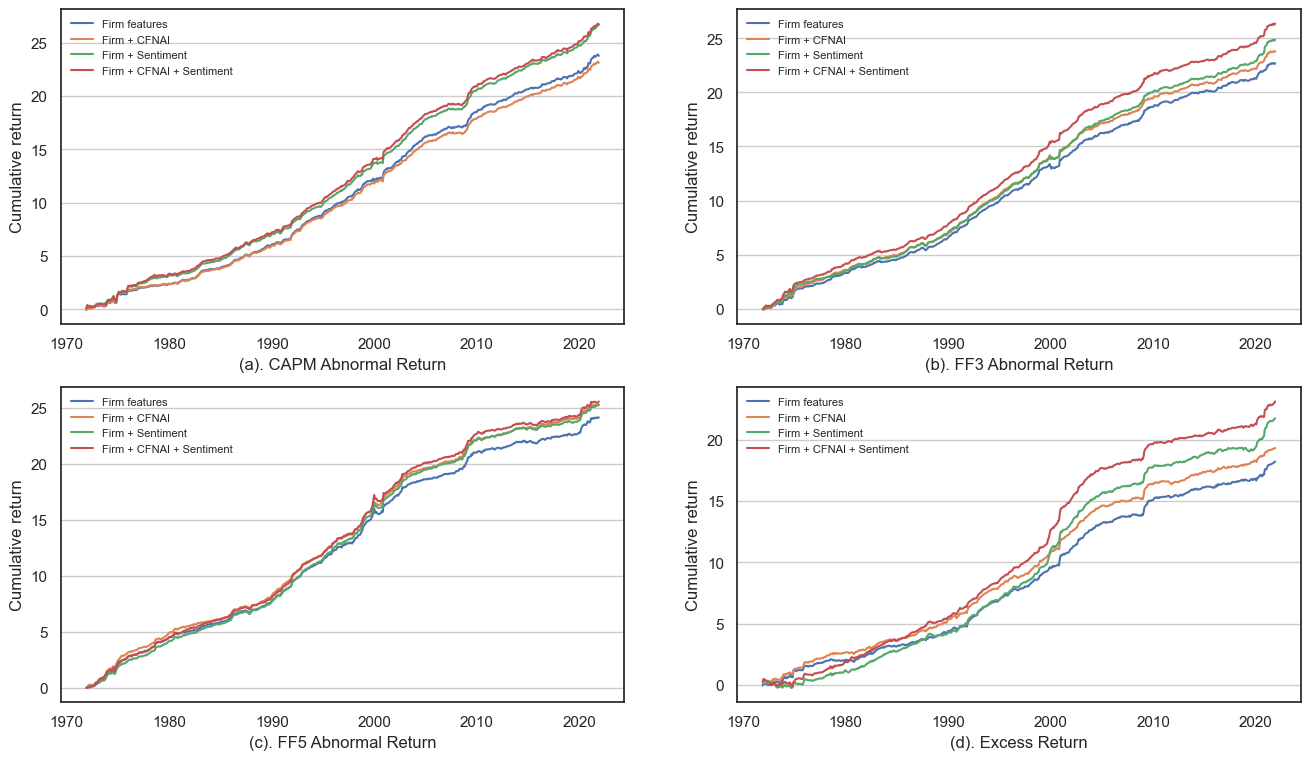
\includegraphics[width=.8\textwidth]{images/ls_portfolios_predictions.png}
  \label{fig: ls portfolios based on prediction}
  \caption*{\footnotesize{This graphic shows the cumulative return of long-short equal weighted portfolios based on predictions with only different conbinations of predictors.}}
\end{figure}
%%%%%%%%%%%%%%%%%%%%%%%%%%%%%%%%%%%%%%%%%%%%%%%%%%%%%%%%%%%%%%%%%%%%
\subsubsection{Feature Importance}

Next, we explore the relative importance of individual firm specific characteristics contributing to the final predicted outputs, as we have discussed in section \ref{subsec:feature importance} and also describled by \citet*{lundberg2018explainable}. Here we take the 3rd observation in the testing dataset as an example, as presented in figure \ref{fig: feature force 1st}, the actual output value of this observation is between (0, 0.02), and the model predicted return based on all the firm characteristics of this single observation is -0.06. The length of the force bar indicating how much a firm feature contributes to the predicted value, and the color represents whether a specific firm feature pushes the predicted output above or below the actual output value. In this case, the stock's Long Term Reversal (LRreversal) contributes the most to the predicted output, and followd by stock's Short Term Reversal (STreversal) and Beta. And features like Intermediate Momentum (IntMon), Momentum 12 Month (Mon12m), and Beta, etc,. push the predicted value above the actual output value. While, features like Long Term Reversal (LRreversal), Short Term Reversal (STreversal), Momentum Based on FF3 Residual (ResidualMomentum), etc,. push the predicted value below the actual output.

\begin{figure}[H]
  \centering
  \caption{\textbf{SHAP Feature Force No.1}}
  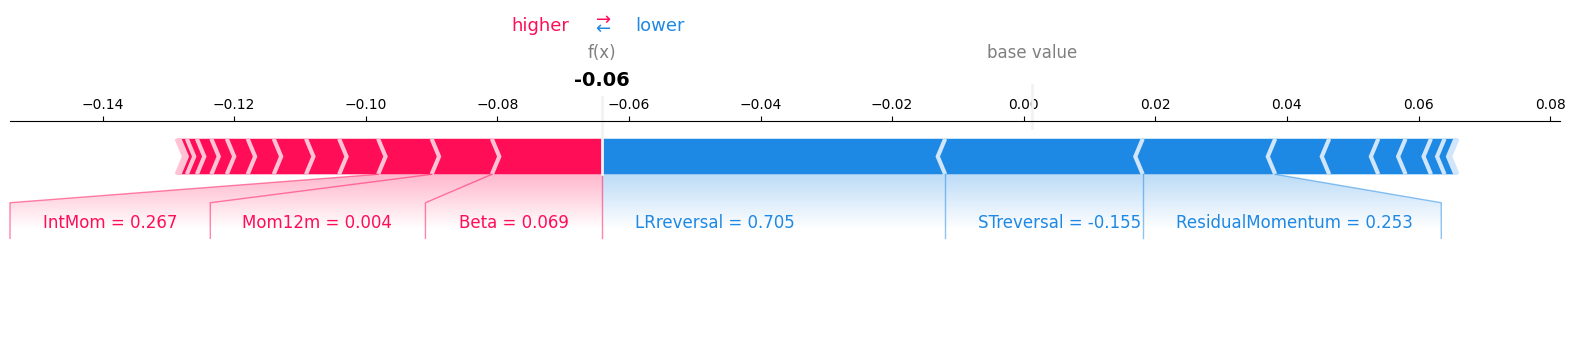
\includegraphics[width=.8\textwidth]{images/3rd_shap_feature_force.png}
  \caption*{\footnotesize{This graphic visulizes how each specific firm features contribute to the final predicted output. The numerical digits behind each features are the actual input values after scaling rounded to 3 decimals. The range is not necessarily between (-1,1), since we build the scaler based on the train data to scale all the train, validation and testing datasets.}}
  \label{fig: feature force 1st}
\end{figure}

Worth to mention that this one observation example does not represent the overall trending in the whole test sample. As you can see in figure \ref{fig: feature force 2nd} the contribution order of firm characteristics has changed for another observation. In this example, LRreversal and STreversal still contribute the most for predicting the output value of this observation, but instead of pushing the predicted stock return below the actual value, STreversal pushes the predicted stock return above the actural value in this example.

\begin{figure}[H]
  \centering
  \caption{\textbf{SHAP Feature Force No.2}}
  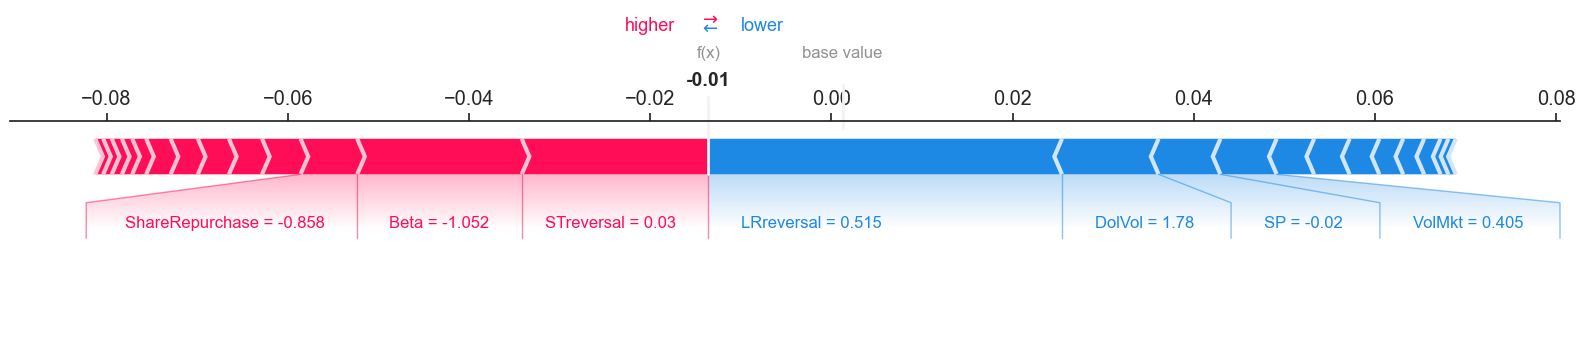
\includegraphics[width=.8\textwidth]{images/4th_shap_feature_force.png}
  \label{fig: feature force 2nd}
\end{figure}

Finally, we combine all the individual observations' Shap value to get the overall feature importance ranking as presented in Figure \ref{fig: feature importance ff5 ab}, for detailed explaination refering to \citet*{lundberg2017unified}. Panel (a) in the figure shows each firm variable's importance for predicting stock abnormal return, among which Short Term Reversla (STreversal) is the most important firm characteristic feature variable, followd by Past Trading Volumn (DolVol), 52 Weeks Trading High (High52) and Market Leverage (Leverage). In panel (b), we compute the mean Shap value within each group. The most important stock characteristic group is stock momentum, followd by trading fraction and macroeconomic variable investors sentiment, we have summarized the detailed group information in table \ref{table: Firm Characteristics by Category}.

\begin{figure}[H]
  \centering
  \caption{\textbf{Shap Feature Importance for FF5 Abnormal Return}}
  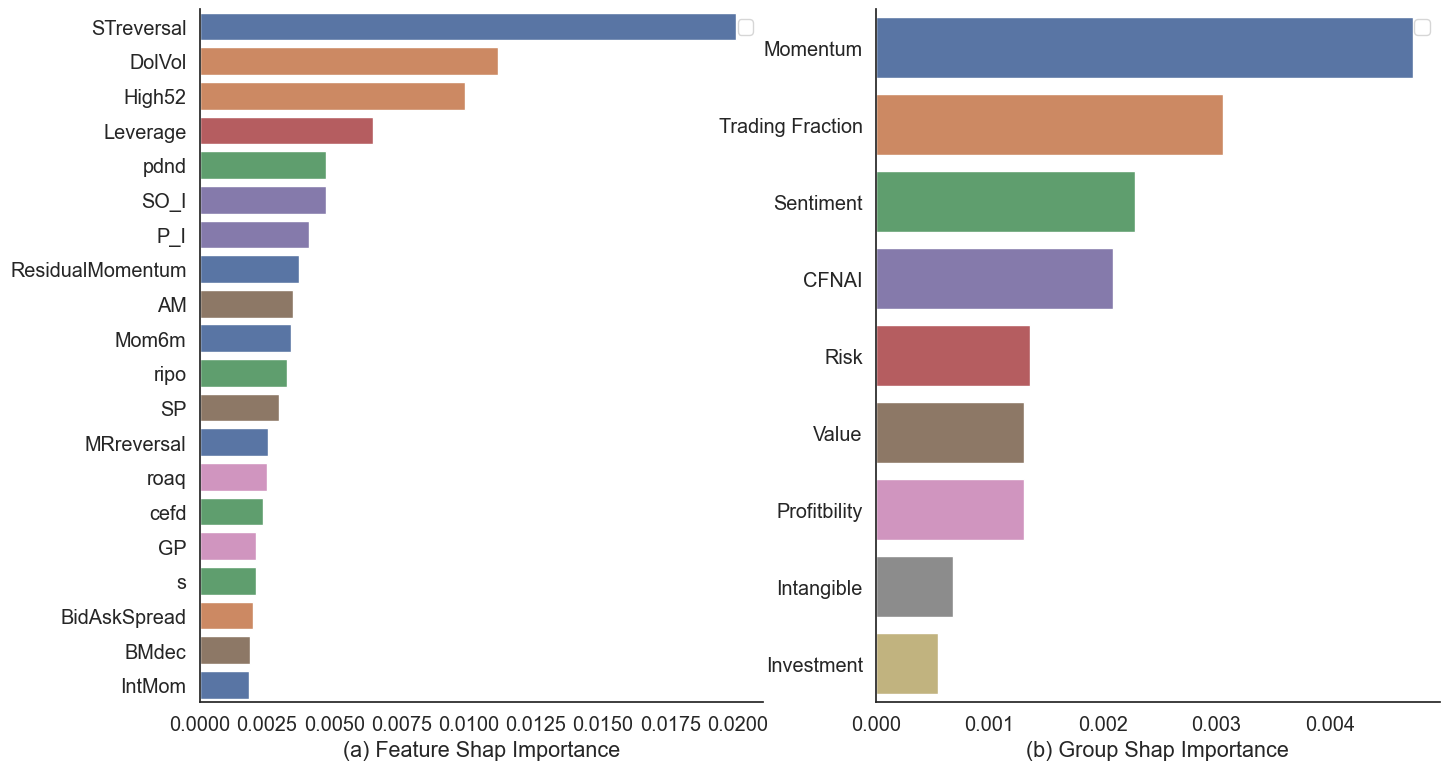
\includegraphics[width=.8\textwidth]{images/shap_feature_importance_ff5.png}
  \label{fig: feature importance ff5 ab}
  \caption*{\footnotesize{This figure shows the importance ranking for predictor variables and variable groups in predicitng stock abnormal returns derived FF5 factor model. The ranking is the average of the feature variables' Shap force. The variable importance measures are evaluated on the testing dataset. Group shap importance is the feature importance's sum value within each group.}}
\end{figure}

In the previous section, we declare that macroeconomic data is far more helpful in predicting stock excess return comparing to stock abnormal return based on the R-squared value. Figure \ref{fig: feature importance ex} dipicts Shap feature importance for stock excess return. Comparing it with figure \ref{fig: feature importance ff5 ab}, the ranking of variables importance has changed and macroeconomic variables ranked to the top above momentum, once again confirm that macroeconomic variables are extremly important for predicting stock excess return comparing to stock abnormal return. Remember equation \ref{eqn:abnormal return 1} and \ref{eqn:abnormal return 2}, stock abnormal return is defined as the alpha derived from factor model while stock excess return is just stock's log return in excess of risk free rate. The reason why stock abnormal return is not so relevant with macroeconomic data is probably because the factor model can capture some macroeconomic information, and it has been removed by the factor models\footnote{Feature importance for predicting stock abnormal returns derived from CAPM model and FF3 model are also presented in Appendix \ref{sec:appendixb3}.}.

\begin{figure}[H]
  \centering
  \caption{\textbf{Shap Feature Importance for Excess Return}}
  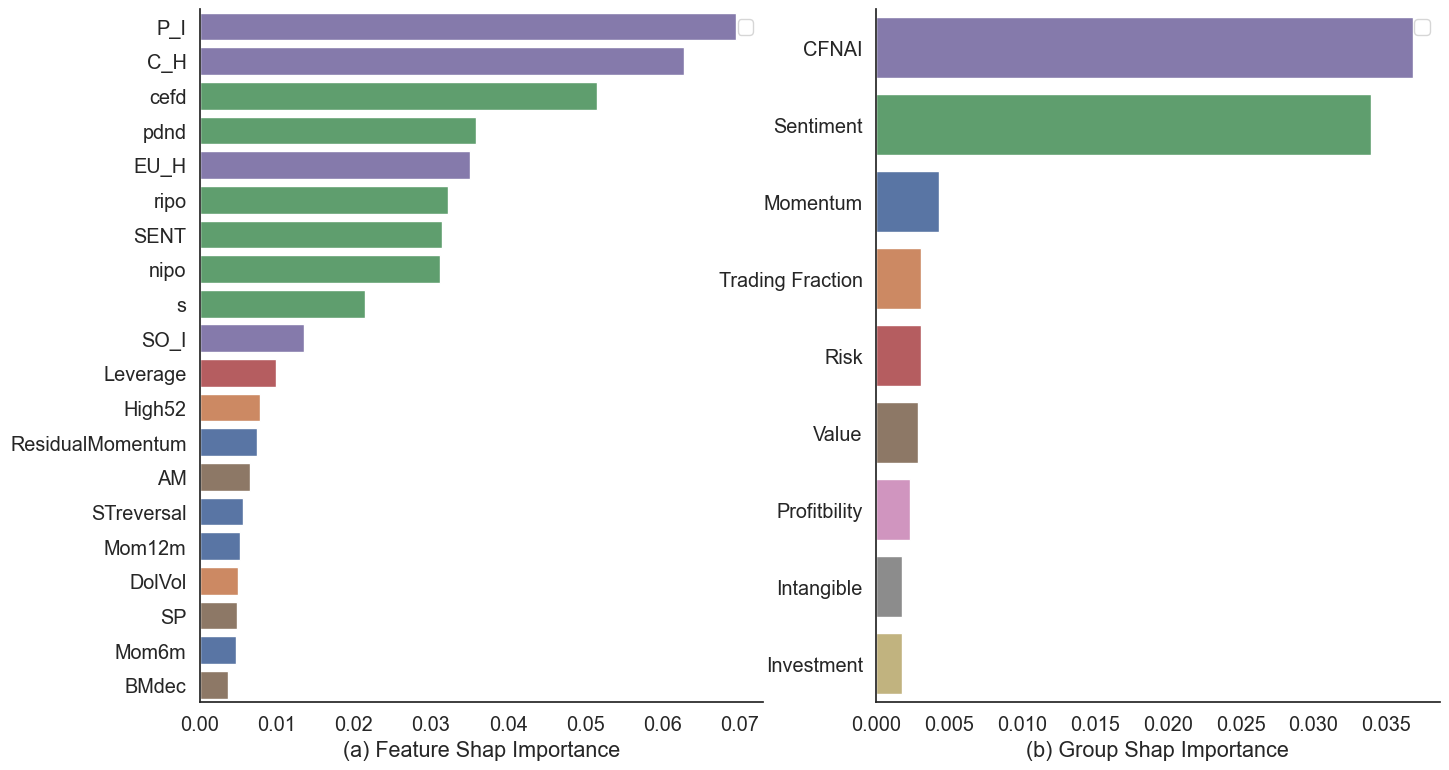
\includegraphics[width=.8\textwidth]{images/shap_feature_importance_ex.png}
  \label{fig: feature importance ex}
  \caption*{\footnotesize{This figure shows the importance ranking for predictor variables and variable groups in predicitng stock excess returns. The ranking is the average of the feature variables' Shap force. The variable importance measures are evaluated on the testing dataset. Group shap importance is the feature importance's sum value within each group.}}
\end{figure}
%%%%%%%%%%%%%%%%%%%%%%%%%%%%%%%%%%%%%%%%%%%%%%%%%%%%%%%%%%%%%%%%%%%

\subsubsection{Macroeconomic Variable Interaction Effects}

Neural network models have advantages accommodating potential complex interaction effects among predictors over other models. We have unveiled the tip of iceberg in section \ref{sec: univariate ls portfolios}, here we step deeper exploring the interaction effects between macroeconomic variable CFNAI index and firm characteristic features that are captured by neural network model. Figure \ref{fig: interaction effect_ex} plots a set of pairwise interaction effects captured by the neural network, it shows how expected stock return vary when we keep all other firm characteristic features fixed at their median value from the testing dataset simultaneously change one firm characteristic feature over the range (-1, 1) and different quantile values of CFNAI index. 

The upper left figure shows how the variable 52 Weeks Trading High (High52) affects predicted stock excess return, the non-linear relationship between this variable and stock excess return is captured by the neural network model, and the CFNAI index put different infuluence on the predicted stock return along with the change of this variable. It shows the macroeconomic condition (we consider CFNAI index proxies macroeconomic conditions) is more significant when the value of variable High52 is low. The interaction effects between variable High52 and CFNAI is clearly observed in this figure, worth to mention that if there is no interaction effects between these two variables the lines of different CFNAI level should be paralle. In panel (b), (c), (d), we also observe the similar interaction effects among CFNAI and momentum based on FF3 residuals (ResidualMomentum), medium‐run reversal (MRreversal), and short-term reversal (STreversal).

\begin{figure}[H]
  \centering
  \caption{\textbf{Interaction Effects Between Firm Features and CFNAI, Excess}}
  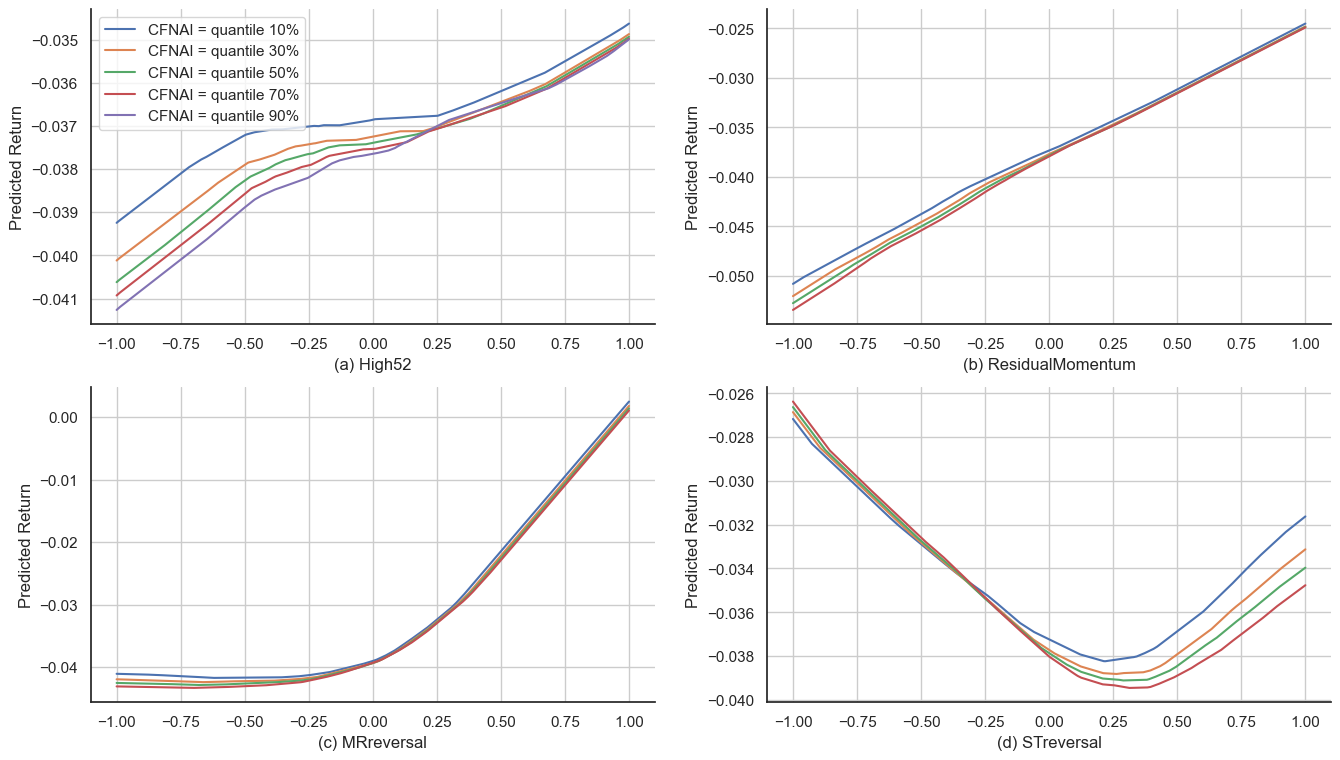
\includegraphics[width=.8\textwidth]{images/interactive_effect_excess.png}
  \label{fig: interaction effect_ex}
  \caption*{\footnotesize{This graphic shows the predicted stock excess return as a function of one stock characteristic feature variable, High52 (52 weeks trading high), ResidualMomentum (Momentum based on FF3 residuals  ), MRreversal (Medium‐run reversal), STreversal (Short term reversal) accordingly. The 'one' variable has a range between(-1, 1), macroeconomic variable CFNAI is seperated at 10\%, 30\%, 50\%, 70\%, and 90\% level. All other variables are fixed with the median value in the testing dataset.}}
\end{figure}

We also plot the interaction effects between the same variables and CFNAI index from the predicton of stock abnormal return derived from FF5 factors model in figure \ref{fig: interaction effect_ff5}. The interaction effect is not as strong as the predicton of stock excess return. In the figure, we could not observe clear interaction effects among these variables and CFNAI index. The reason behind again is that stock abnormal returns are not so relevant with macroeconomic conditions, which have been removed by factor models as we have discussed before.

\begin{figure}[H]
  \centering
  \caption{\textbf{Interaction Effects Between Firm Features and CFNAI, FF5}}
  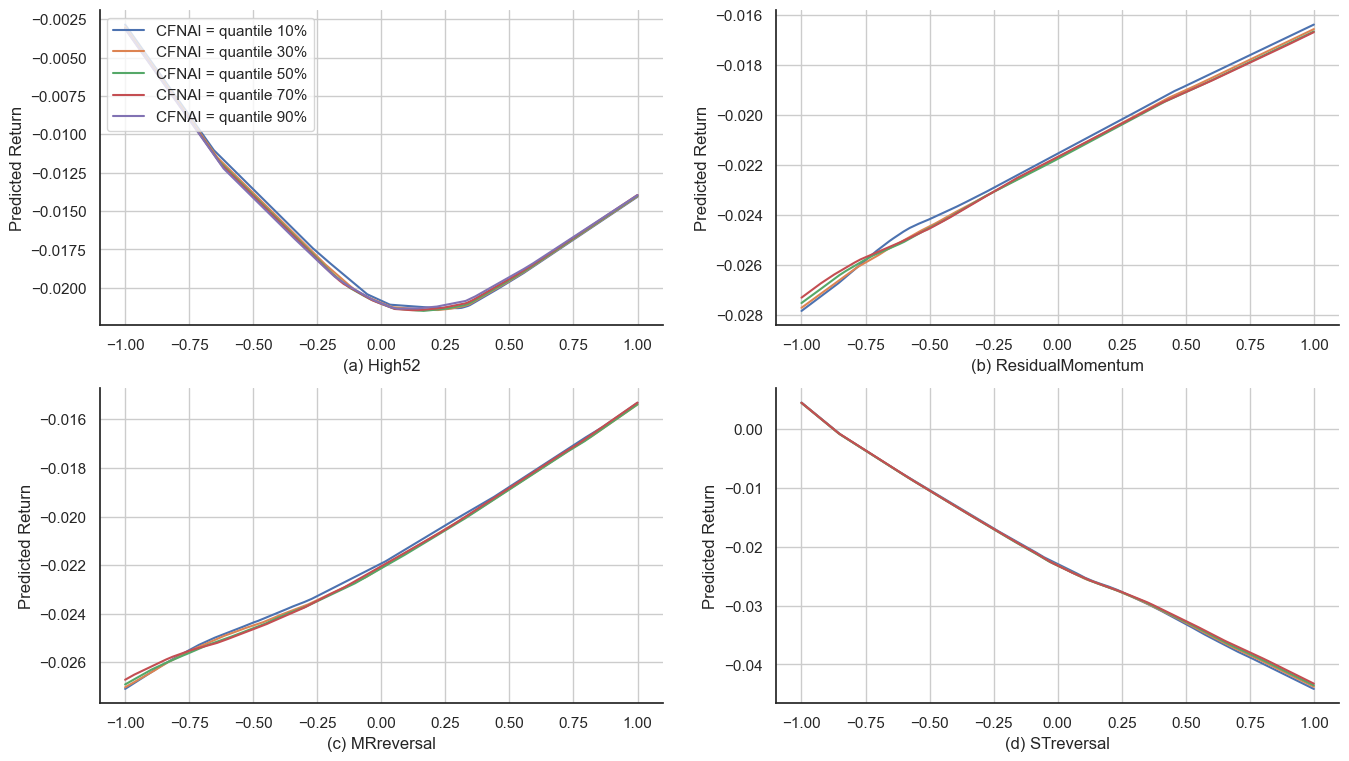
\includegraphics[width=.8\textwidth]{images/interactive_effect_ff5.png}
  \label{fig: interaction effect_ff5}
  \caption*{\footnotesize{This graphic shows the predicted stock abnormal return derived from FF5 factors model as a function of one stock characteristic feature variable, High52 (52 weeks trading high), ResidualMomentum (Momentum based on FF3 residuals  ), MRreversal (Medium‐run reversal), STreversal (Short term reversal) accordingly. The 'one' variable has a range between(-1, 1), macroeconomic variable CFNAI is seperated at 10\%, 30\%, 50\%, 70\%, and 90\% level. All other variables are fixed with the median value in the testing dataset.}}
\end{figure}

%%%%%%%%%%%%%%%%%%%%%%%%%%%%%%%%%%%%%%%%%%%%%%%%%%%%%%%%%%%%%%%%%%%
\subsubsection{Market Timing Based on Macroeconomic Conditions}

The interaction effects between macroeconomic conditions and firm feature variables have been shown to be strong, as demonstrated by the univariate long-short portfolios in Section \ref{sec: univariate ls portfolios} and the analysis above. Given this finding, the question arises as to whether the model prediction-based portfolios can achieve varying returns in different macroeconomic conditions, which would enable investors to identify optimal market timing for investment. Table \ref{table: portfolio ret in tertiles} shows the out-of-sample long-only portfolios' performance in different macroeconomic conditions. The portfolios are formulated based on the sorting of next-month model-predicted returns into deciles. We divide the CFNAI index into tertiles and define the bottom to top tertile as a recession, normal, and expansion period respectively. Within each period, the long-only portfolios achieve a clear increase in the mean portfolio's return for both stock abnormal and excess returns, which confirms that the model prediction-based portfolios are distinguished from bad to good. When considering Sharpe ratios instead of mean returns, the evidence is nearly identical, with higher deciles achieving higher Sharpe ratios than lower deciles in most cases. These results suggest that the model prediction-based portfolios may offer value to investors seeking to optimize their investment decisions by considering macroeconomic conditions.

Comparing the results horizontally in both Panel (a) and Panel (b), the top decile (portfolio decile\_10) achieves higher mean returns and Sharpe ratios in recession periods when the CFNAI index in low. This result coincides once again with the univariate long-short portfolios' performance discussed in Section \ref{sec: univariate ls portfolios}. The result simply indicating that investors who want to invest during recession period, when the market is more volatile, can earn higher abnormal and excess returns than with the same strategy during other periods, when the market is more stable. The same observations are presented in the Appendix \ref{sec:appendixb5} for stock abnormal returns derived from CAPM and FF3 factors models.

\begin{table}[H]
  \centering
  \caption{\textbf{Prediction Based Portfolios' Return in Defferent Macroeconomic Conditions}}
  \begin{tabular}{l|cc|cc|cc}
  \hline
      \multicolumn{7}{c}{(a) Portfolios' FF5 Abnormal Return (Mean)}\\\hline
      ~ & \multicolumn{2}{c}{Recession} & \multicolumn{2}{c}{Normal} & \multicolumn{2}{c}{Expansion} \\ \cline{2-7}
      Portfolios & Mean & Sharpe Ratio & Mean & Sharpe Ratio & Mean & Sharpe Ratio \\ \hline
      Decile\_1 & -1.779 & -0.367 & -1.823 & -0.443 & -1.564 & -0.347 \\ 
      Decile\_2 & -0.634 & -0.221 & -0.812 & -0.407 & -0.925 & -0.385 \\ 
      Decile\_3 & -0.716 & -0.292 & -0.348 & -0.234 & -0.533 & -0.221 \\ 
      Decile\_4 & -0.438 & -0.204 & -0.304 & -0.170 & -0.170 & -0.070 \\ 
      Decile\_5 & -0.179 & -0.070 & -0.148 & -0.088 & -0.135 & -0.054 \\ 
      Decile\_6 & 0.156 & 0.057 & 0.074 & 0.038 & -0.005 & -0.002 \\ 
      Decile\_7 & 0.220 & 0.074 & 0.323 & 0.161 & 0.031 & 0.015 \\ 
      Decile\_8 & 0.242 & 0.067 & 0.410 & 0.185 & 0.524 & 0.182 \\ 
      Decile\_9 & 1.199 & 0.256 & 0.923 & 0.300 & 0.958 & 0.288 \\ 
      Decile\_10 & 2.971 & 0.390 & 2.173 & 0.421 & 2.424 & 0.455 \\  \hline

      \multicolumn{7}{c}{(b) Portfolios' Excess Return (Mean)}\\\hline
      ~ & \multicolumn{2}{c}{Recession} & \multicolumn{2}{c}{Normal} & \multicolumn{2}{c}{Expansion} \\ \cline{2-7}
      Portfolios & Mean & Sharpe Ratio & Mean & Sharpe Ratio & Mean & Sharpe Ratio \\ \hline
      Decile\_1 & -0.345 & -0.048 & -0.450 & -0.072 & -0.380 & -0.052 \\ 
      Decile\_2 & 0.554 & 0.085 & 0.289 & 0.060 & -0.153 & -0.025 \\ 
      Decile\_3 & 0.461 & 0.075 & 0.485 & 0.110 & 0.138 & 0.025 \\ 
      Decile\_4 & 0.588 & 0.094 & 0.515 & 0.121 & 0.259 & 0.047 \\ 
      Decile\_5 & 0.703 & 0.108 & 0.661 & 0.144 & 0.305 & 0.051 \\ 
      Decile\_6 & 1.124 & 0.160 & 0.773 & 0.159 & 0.380 & 0.064 \\ 
      Decile\_7 & 1.263 & 0.175 & 0.957 & 0.196 & 0.373 & 0.061 \\ 
      Decile\_8 & 1.252 & 0.153 & 0.987 & 0.197 & 0.645 & 0.097 \\ 
      Decile\_9 & 2.094 & 0.241 & 1.303 & 0.244 & 0.978 & 0.138 \\ 
      Decile\_10 & 3.938 & 0.320 & 2.213 & 0.327 & 2.185 & 0.252 \\ \hline
  \end{tabular}
  \label{table: portfolio ret in tertiles}
  \begin{tablenotes}
    \footnotesize
    \item This table presents the actual mean portfolios' return and sharpe ratio in different macroeconomic conbinations. Portfolios are sorted based on the predicted abnormal and excess stock return made by neural network model. Macroeconomic conbinations defined as recession period, normal period, and expansion period based on the CFNAI index.
  \end{tablenotes}
\end{table}

%%%%%%%%%%%%%%%%%%%%%%%%%%%%%%%%%%%%%%%%%%%%%%%%%%%%%%%%%%%%%%%%%%%

%%%%%%%%%%%%%%%%%%%%%%%%%%%%%%%%%%%%%%%%%%%%%%%%%%%%%%%%%%%%%%%%
%%%%%%%%%%%%%%%%%%%%%%%%%%%%%%%%%%%%%%%%%%%%%%%%%%%%%%%%%%%%%%%%
\section{Conclusion} \label{sec:conclusion}
In this research paper, we re-examine the longstanding yet ever-relevant question in empirical asset pricing of predicting stock returns. Our study adds to the existing body of empirical asset pricing literature in several significant ways. Firstly, predicting stock returns is a challenging task, as it involves accounting for the interaction effects between various predictors and the non-linear relationships present in the underlying mapping function. Traditional linear models are unable to account for these complexities, while modern neural network models have shown to possess superior capabilities in capturing these interactions and non-linearities. This study offers a comprehensive guide on utilizing deep neural network models to predict stock returns. The guide covers crucial aspects, such as determining the appropriate model settings to achieve specific objectives, understanding the impact of each hyperparameter on the model's performance, and optimizing hyperparameters to enhance the predictive accuracy of the model.

Secondly, our study distinguishes itself from most empirical studies in this area by examining the predictability of different versions of stock abnormal returns and stock excess return. Specifically, we define stock abnormal returns as the alpha of CAPM, Fama-Frech 3 factors, and Fama-Frech 5 factors model in predicting excess returns, representing the difference between the model's expected stock returns and the actual stock excess returns. We find that, using the same information set, the model shows nearly the same predicting power in predicting different measures of stock returns. In fact, our results indicate that the out-of-sample R-squared values for predicting stock abnormal and excess are almost identical.

Thirdly, we incorporate macroeconomic variables CFNAI and investor sentiment data to capture the macroeconomic conditions. Our analysis reveals a strong interaction effect between these macroeconomic index variables and firm characteristic variables when predicting stock excess return. Adding these macroeconomic variables, along with the 49 firm characteristic variables to the neural network model, significantly improves the out-of-sample R-Squared value for predicting stock excess returns. However, we observe that the interaction effects are not as prominent when predicting stock abnormal return. This is primarily because the factors models has already eliminated the time trend associated with macroeconomic flatulation in the stock abnormal return.

Finally, we divide the entire dataset into three subperiods, namely recession, normal, and expansion periods based on the CFNAI index. The significant interaction effects observed between the macroeconomic index variables and firm characteristic variables indicate that stock returns vary across different macroeconomic conditions. Our analysis reveals that the model-predicted portfolios generate higher mean returns and Sharpe ratios during recession period when the market is more volatile, while they perform relatively lower during normal and expansion periods when the market is less volatile. This finding provides valuable insights into identifying the optimal market timing for investment decisions.

\clearpage
%%%%%%%%%%%%%%%%%%%%%%%%%%%%%%%%%%%%%%%%%%%%%%%%%%%%%%%%%%%%%%%%
%%%%%%%%%%%%%%%%%%%%%%%%%%%%%%%%%%%%%%%%%%%%%%%%%%%%%%%%%%%%%%%%
\begingroup
\setstretch{1.0}
\bibliographystyle{plainnat}
\bibliography{citation}
\endgroup

\clearpage
%%%%%%%%%%%%%%%%%%%%%%%%%%%%%%%%%%%%%%%%%%%%%%%%%%%%%%%%%%%%%%%%
%%%%%%%%%%%%%%%%%%%%%%%%  Appendix  %%%%%%%%%%%%%%%%%%%%%%%%%%%%
%%%%%%%%%%%%%%%%%%%%%%%%%%%%%%%%%%%%%%%%%%%%%%%%%%%%%%%%%%%%%%%%
% By default figure number is continuous on appendix. You can change this by the following two lines
\setcounter{figure}{0}
\setcounter{table}{0}
\renewcommand\thetable{\Alph{section}.\arabic{table}}
\renewcommand\thefigure{\Alph{section}.\arabic{figure}}

\section*{Appendix A. Data} \label{sec:appendixa}
\addcontentsline{toc}{section}{Appendix A}
\subsection*{A1. Stock Return Data}\label{sec:appendixa1}

\begin{table}[!ht]
  \centering
  \caption{\textbf{Summary Statistics of Stock Returns}}
  \begin{tabular}{lcccc}
  \hline
      ~ & CAPM ab\_return & FF3 ab\_return & FF5 ab\_return & Excess return \\ \hline
      Count & 1397937 & 1397937 & 1397937 & 1397937 \\ 
      Mean & 0.001 & 0.000 & 0.001 & 0.009 \\ 
      Std & 0.163 & 0.165 & 0.173 & 0.170 \\ 
      Min & -2.306 & -2.748 & -4.295 & -0.985 \\ 
      25\% & -0.070 & -0.072 & -0.074 & -0.067 \\ 
      50\% & -0.007 & -0.008 & -0.007 & -0.002 \\ 
      75\% & 0.057 & 0.058 & 0.062 & 0.069 \\ 
      Max & 18.920 & 18.928 & 19.043 & 18.998 \\ \hline
  \end{tabular}
  \label{table: Summary statistic of return}
\end{table}

\begin{figure}[H]
  \centering
  \caption{\textbf{Correlation Between Stock Returns}}
  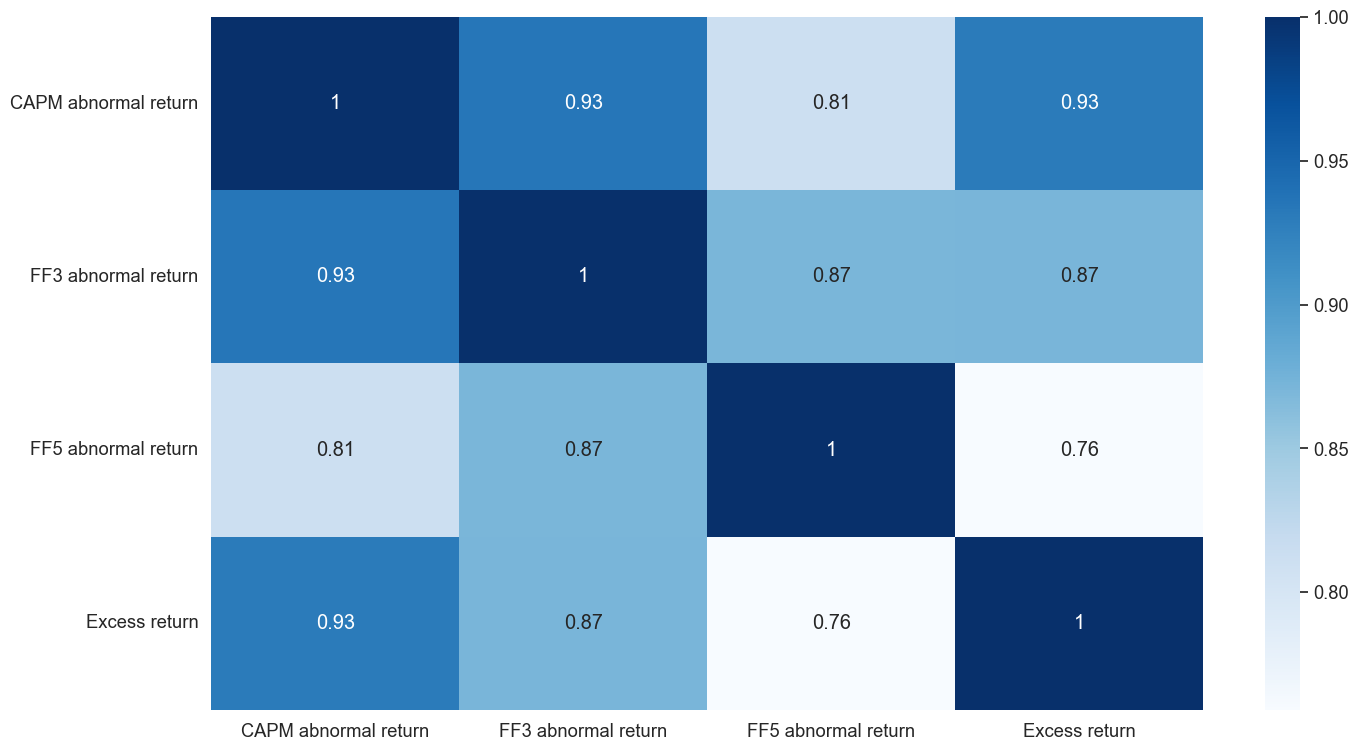
\includegraphics[width=.8\textwidth]{images/abnormal_excess_corr.png}
  \label{fig: abnormal_excess_corr}
  \caption*{\footnotesize{This figure plots the heatmap of correlations among each different measurements of stock returns.}}
\end{figure} 

\subsection*{A2. Macroeconomic Data}\label{sec:appendixa2}
The CFNAI index is composed of 85 economic indicators, it also includes indices covering four broad categories:
\begin{itemize}
  \item Production and income: measures of output, income, and sales, including indicators such as industrial production, personal income, and manufacturing and trade sales.

  \item Employment, unemployment, and hours: measures of labor market activity, including indicators such as nonfarm payrolls, unemployment rate, and average weekly hours.
  
  \item Personal consumption and housing: measures of consumer spending and housing activity, including indicators such as retail sales, housing starts, and new home sales.
  
  \item Sales, orders, and inventories: measures of business activity, including indicators such as durable goods orders, wholesale trade inventories, and new orders for nondefense capital goods.
\end{itemize}

\begin{figure}[H]
  \centering
  \caption{\textbf{Subsectional Macroeconomic indices}}
  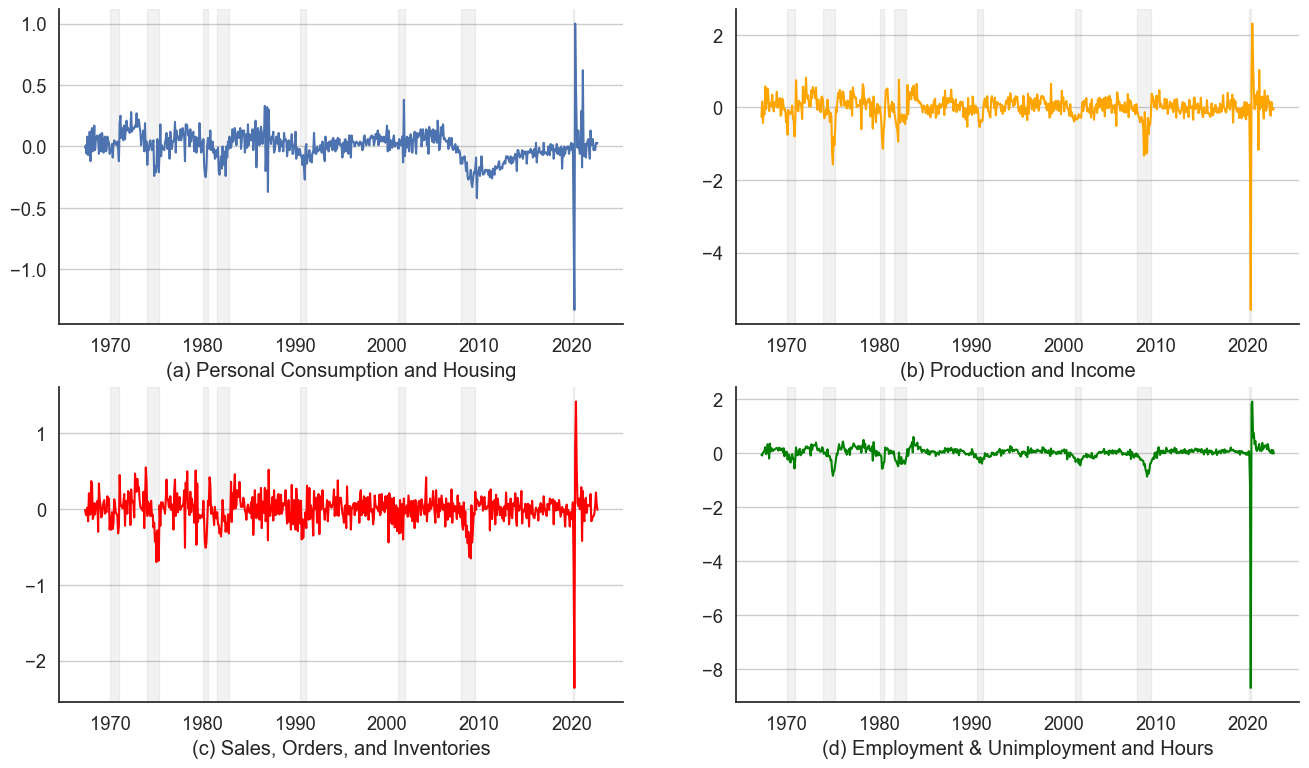
\includegraphics[width=.8\textwidth]{images/cfnai_four_components.png}
  \label{fig: Subsectional Macroeconomic index}
  \caption*{\footnotesize{This figure plots the subsectional macroeconomic indices from the CFNAI index dataset together with the NBER suggested recession periods with shaded bars.}}
\end{figure} 

The investor's sentiment data is composed by five indicators including:

\begin{itemize}
  \item Dividend premium: measures the difference between the value-weighted dividend yield of stocks and the yield on long-term government bonds.
  \item First day return on IPO: measures the percentage change in stock price from the offer price to the first day of trading.
  \item Closed-end fund discount: measures the difference between the market price and the net asset value of a closed-end fund.
  \item IPO valume: measures the number of new issues in a month.
  \item Equity share in new issues: measures the percentage of new issues in which the issuing company retains less than half of the outstanding equity.
\end{itemize}

\begin{figure}[H]
  \centering
  \caption{\textbf{5 Components for Composing Sentiment Index}}
  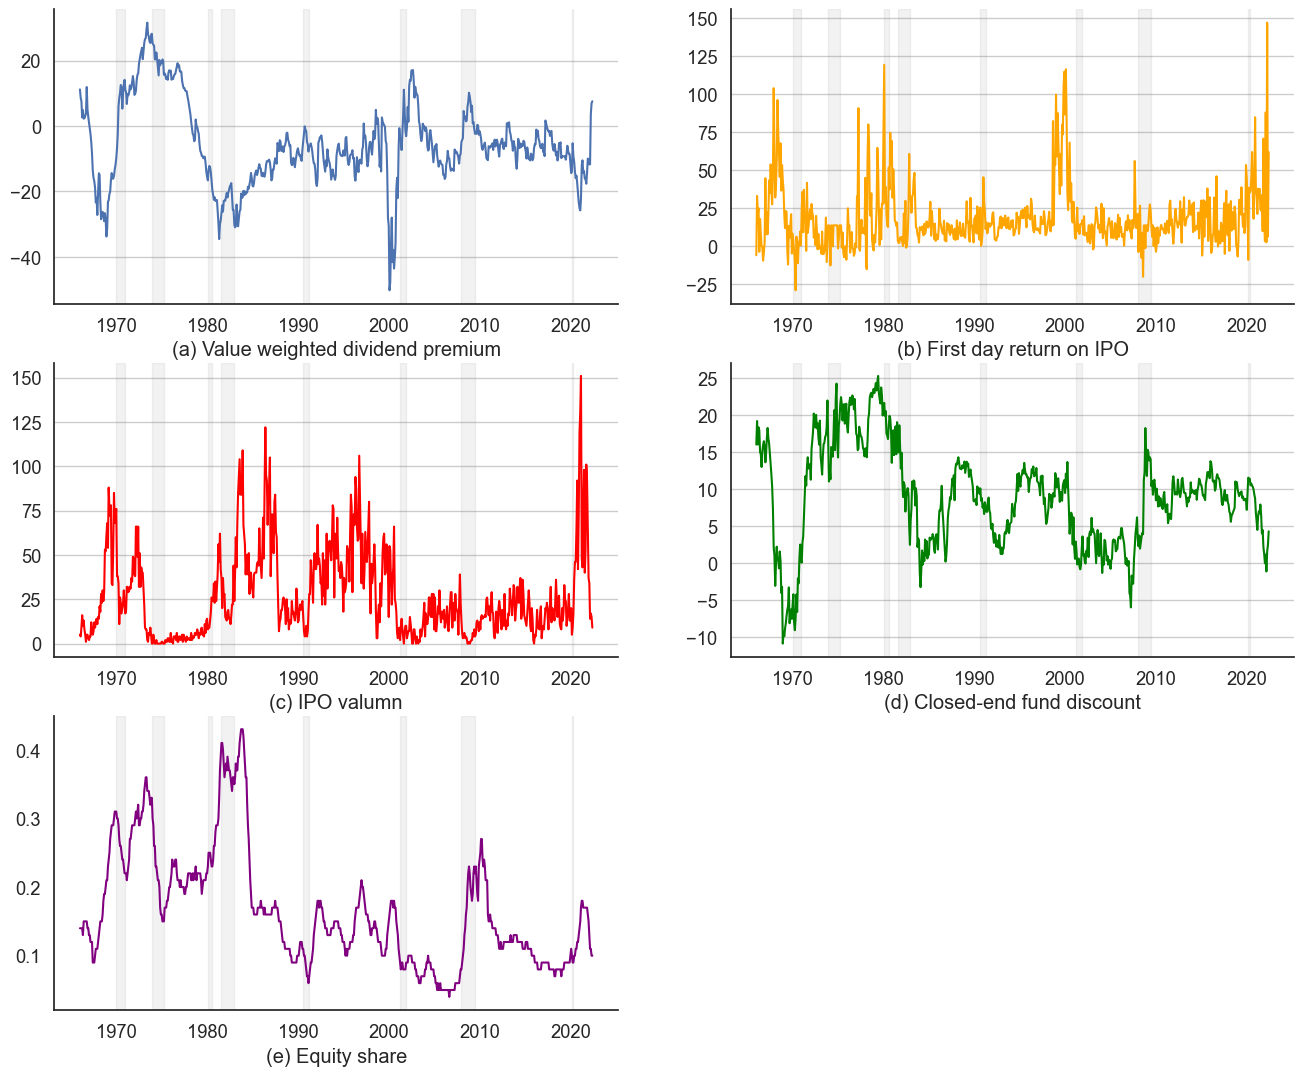
\includegraphics[width=.8\textwidth]{images/sent_5_components.png}
  \label{fig: 5 components for sentiment}
  \caption*{\footnotesize{This figure plots the 5 components for composing investor's sentiment index together with the NBER suggested recession periods with shaded bars.}}
\end{figure} 

\section*{Appendix B. Robust Result} \label{sec:appendixb}
\addcontentsline{toc}{section}{Appendix B}
\subsection*{B1. Robust Result for Univariate Long-short Portfolios}\label{sec:appendixb1}

\begin{figure}[H]
  \centering
  \caption{\textbf{CAPM Abnormal Return: Univariate Long-short Portfolios' Cumulative Return}}
  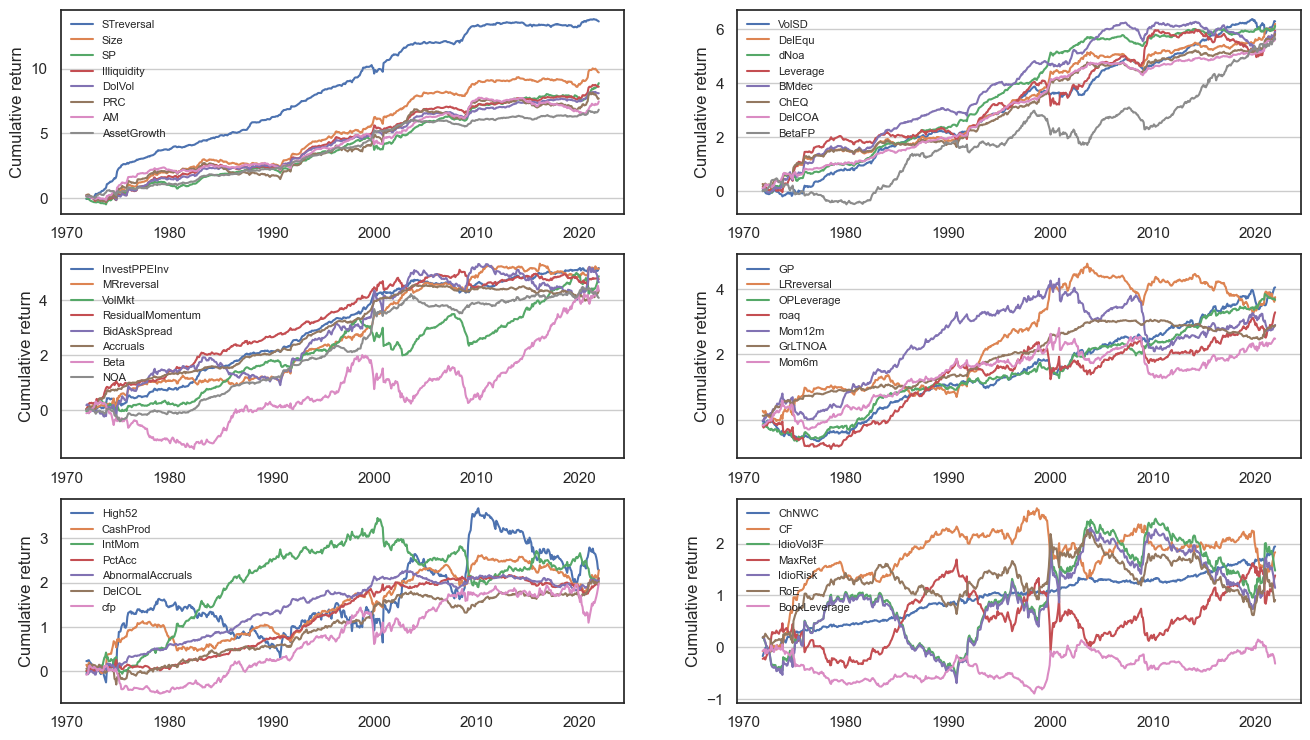
\includegraphics[width=.8\textwidth]{images/univariate_ls_cum_ret_capm.png}
  \label{fig: capm univariate ls cumulative return}
  \caption*{\footnotesize{This graphic showcases firm characteristics sorted univariate long-short portfolios' cumulative return acrossing the whole time period, the return refering to the abnormal return derived from CAPM factor model.}}
\end{figure}

\begin{figure}[H]
  \centering
  \caption{\textbf{CAPM Abnormal Return: Univariate Long-short Portfolios Performance in Different Macroeconomic Conditions}}
  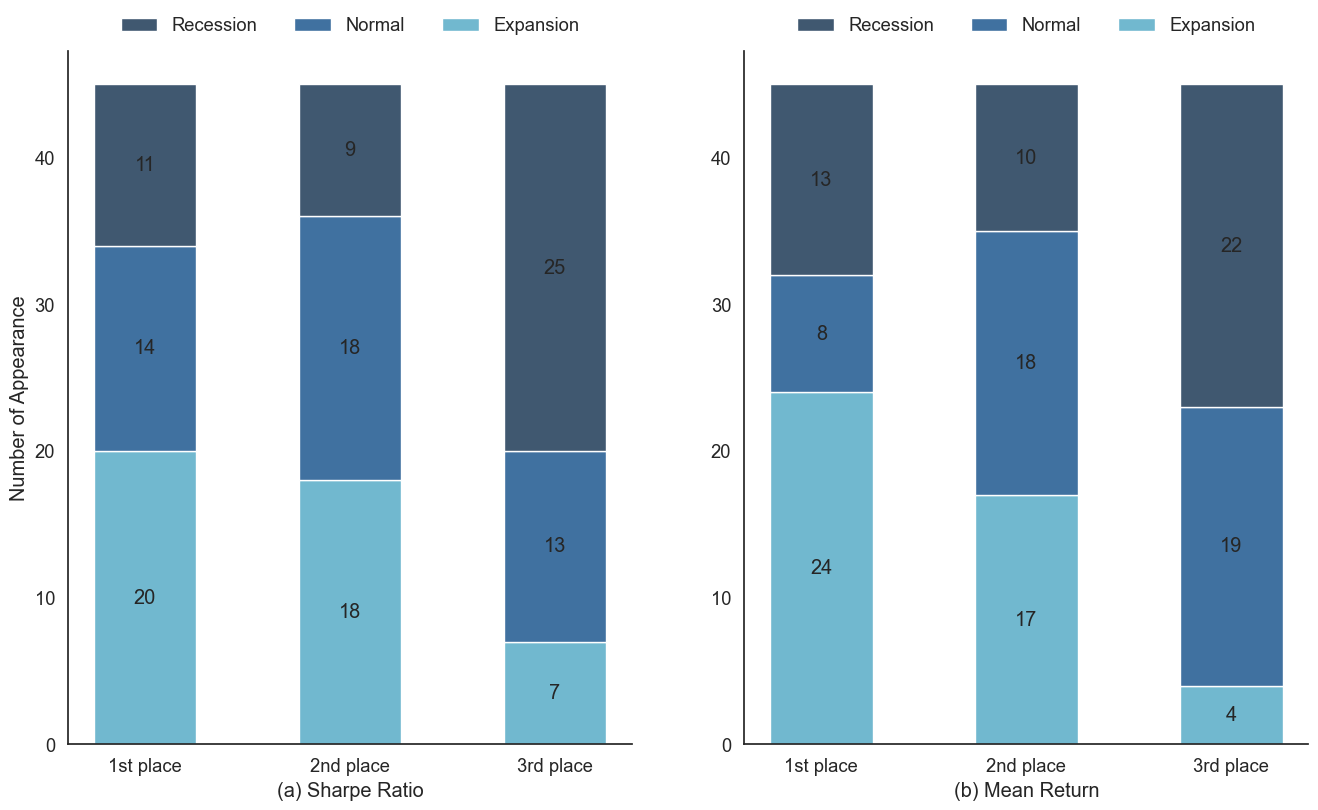
\includegraphics[width=.8\textwidth]{images/univariant_ls_capm_comparing.png}
  \label{fig: capm univariate ls comparing}
  \caption*{\footnotesize{This graphic showcases firm characteristics sorted long-short univariate portfolios' performance across different macroeconomic conditions. We compare univariate long-short portfolios' sharpe ratio and mean return in recession, normal, and expansion periods, which is the horizontal comparision among the last 6 columns in table \ref{table: capm univariate ls portfolio}.}}
\end{figure}

\begin{table}[H]
  \centering
  \footnotesize
  \caption{\textbf{CAPM Abnormal Return: Univariate Long-short Portfolios' Returns}}
  \label{table: capm univariate ls portfolio}
  \begin{tabular}{lcc|cc|cc|cc}
  \hline
      ~ & \multicolumn{2}{c}{Full Sample} & \multicolumn{2}{c}{Recession} & \multicolumn{2}{c}{Normal} & \multicolumn{2}{c}{Expansion} \\
      ~ & SR & Mean & SR & Mean & SR & Mean & SR & Mean \\ \hline
      STreversal & 0.023 & 0.364 & 0.037 & 0.485 & 0.012 & 0.219 & 0.018 & 0.367 \\ 
      Size & 0.010 & 0.302 & 0.009 & 0.258 & 0.008 & 0.272 & 0.013 & 0.372 \\ 
      Illiquidity & 0.009 & 0.289 & 0.008 & 0.224 & 0.007 & 0.279 & 0.013 & 0.366 \\ 
      DolVol & 0.010 & 0.270 & 0.005 & 0.121 & 0.014 & 0.465 & 0.013 & 0.292 \\ 
      High52 & 0.007 & 0.268 & 0.006 & 0.225 & 0.005 & 0.188 & 0.011 & 0.374 \\ 
      PRC & 0.011 & 0.257 & 0.009 & 0.200 & 0.013 & 0.305 & 0.012 & 0.276 \\ 
      SP & 0.009 & 0.253 & 0.007 & 0.185 & 0.008 & 0.303 & 0.010 & 0.304 \\ 
      BidAskSpread & 0.013 & 0.252 & 0.011 & 0.176 & 0.014 & 0.320 & 0.016 & 0.293 \\ 
      NOA & 0.015 & 0.239 & 0.014 & 0.193 & 0.014 & 0.238 & 0.016 & 0.323 \\ 
      VolSD & 0.010 & 0.233 & 0.011 & 0.223 & 0.009 & 0.241 & 0.011 & 0.240 \\ 
      dNoa & 0.010 & 0.228 & 0.011 & 0.231 & 0.007 & 0.202 & 0.011 & 0.248 \\ 
      InvestPPEInv & 0.014 & 0.225 & 0.012 & 0.178 & 0.015 & 0.293 & 0.015 & 0.228 \\ 
      DelCOA & 0.016 & 0.223 & 0.018 & 0.227 & 0.014 & 0.243 & 0.016 & 0.210 \\ 
      AssetGrowth & 0.010 & 0.209 & 0.002 & 0.032 & 0.012 & 0.285 & 0.016 & 0.366 \\ 
      AM & 0.008 & 0.194 & 0.005 & 0.098 & 0.006 & 0.199 & 0.013 & 0.314 \\ 
      OPLeverage & 0.005 & 0.187 & 0.003 & 0.121 & 0.003 & 0.150 & 0.008 & 0.273 \\ 
      Accruals & 0.012 & 0.185 & 0.014 & 0.167 & 0.008 & 0.130 & 0.015 & 0.275 \\ 
      GP & 0.009 & 0.177 & 0.011 & 0.203 & 0.005 & 0.137 & 0.009 & 0.180 \\ 
      BookLeverage & 0.007 & 0.166 & 0.011 & 0.250 & 0.004 & 0.091 & 0.006 & 0.147 \\ 
      DelEqu & 0.009 & 0.165 & 0.000 & -0.006 & 0.014 & 0.278 & 0.015 & 0.298 \\ 
      ChEQ & 0.007 & 0.165 & 0.003 & 0.067 & 0.011 & 0.262 & 0.007 & 0.183 \\ 
      Leverage & 0.010 & 0.163 & 0.010 & 0.134 & 0.006 & 0.100 & 0.014 & 0.271 \\ 
      ChNWC & 0.006 & 0.162 & 0.008 & 0.197 & 0.007 & 0.203 & 0.003 & 0.089 \\ 
      roaq & 0.003 & 0.152 & 0.006 & 0.261 & 0.000 & 0.024 & 0.003 & 0.140 \\ 
      MRreversal & 0.013 & 0.148 & 0.021 & 0.209 & 0.008 & 0.114 & 0.009 & 0.105 \\ 
      AbnormalAccruals & 0.003 & 0.146 & 0.005 & 0.189 & 0.000 & -0.009 & 0.005 & 0.218 \\ 
      GrLTNOA & 0.003 & 0.144 & 0.002 & 0.083 & 0.003 & 0.140 & 0.005 & 0.224 \\ 
      IdioVol3F & 0.008 & 0.133 & -0.005 & -0.070 & 0.014 & 0.315 & 0.016 & 0.275 \\ 
      BetaFP & 0.003 & 0.116 & 0.002 & 0.051 & 0.005 & 0.202 & 0.004 & 0.124 \\ 
      IdioRisk & 0.006 & 0.106 & 0.009 & 0.137 & 0.005 & 0.089 & 0.005 & 0.086 \\ 
      ResidualMomentum & 0.008 & 0.098 & 0.011 & 0.126 & 0.003 & 0.050 & 0.008 & 0.103 \\ 
      MaxRet & 0.004 & 0.097 & 0.003 & 0.060 & 0.001 & 0.042 & 0.007 & 0.209 \\ 
      CashProd & 0.005 & 0.090 & 0.000 & -0.006 & 0.011 & 0.216 & 0.006 & 0.103 \\ 
      DelCOL & 0.007 & 0.089 & 0.001 & 0.017 & 0.010 & 0.133 & 0.010 & 0.137 \\ 
      BMdec & 0.004 & 0.074 & -0.002 & -0.033 & 0.006 & 0.144 & 0.007 & 0.155 \\ 
      Beta & 0.005 & 0.071 & -0.004 & -0.051 & 0.011 & 0.196 & 0.009 & 0.166 \\ 
      PctAcc & 0.003 & 0.068 & -0.002 & -0.036 & 0.006 & 0.123 & 0.006 & 0.135 \\ 
      RoE & 0.004 & 0.064 & -0.004 & -0.043 & 0.010 & 0.202 & 0.007 & 0.132 \\ 
      cfp & 0.003 & 0.057 & -0.001 & -0.013 & 0.003 & 0.061 & 0.007 & 0.127 \\ 
      LRreversal & 0.004 & 0.046 & 0.021 & 0.193 & -0.008 & -0.123 & -0.003 & -0.041 \\ 
      CF & 0.002 & 0.034 & 0.001 & 0.010 & 0.002 & 0.032 & 0.004 & 0.058 \\ 
      Mom6m & 0.002 & 0.031 & 0.006 & 0.075 & 0.000 & 0.006 & 0.000 & 0.004 \\ 
      VolMkt & 0.002 & 0.025 & 0.008 & 0.118 & -0.004 & -0.071 & 0.000 & -0.002 \\ 
      Mom12m & 0.002 & 0.024 & 0.006 & 0.071 & 0.000 & -0.001 & 0.000 & -0.005 \\ 
      IntMom & -0.001 & -0.015 & 0.000 & 0.011 & 0.002 & 0.053 & -0.003 & -0.105 \\ \hline
  \end{tabular}
  \begin{tablenotes}
    \footnotesize
    \item This table presents firm characteristics sorted univariate long-short portfolios' sharpe ratios and mean returns. The dataset has futher splitted into three different subsamples based on macroeconomic condition indicator -- CFNAI index, named by recession, normal, and expansion period. The return in this table refering to the abnormal stock return derived from CAPM model.
  \end{tablenotes}
\end{table}

\begin{figure}[H]
  \centering
  \caption{\textbf{FF3 Abnormal Return: Univariate Long-short Portfolios' Cumulative Return}}
  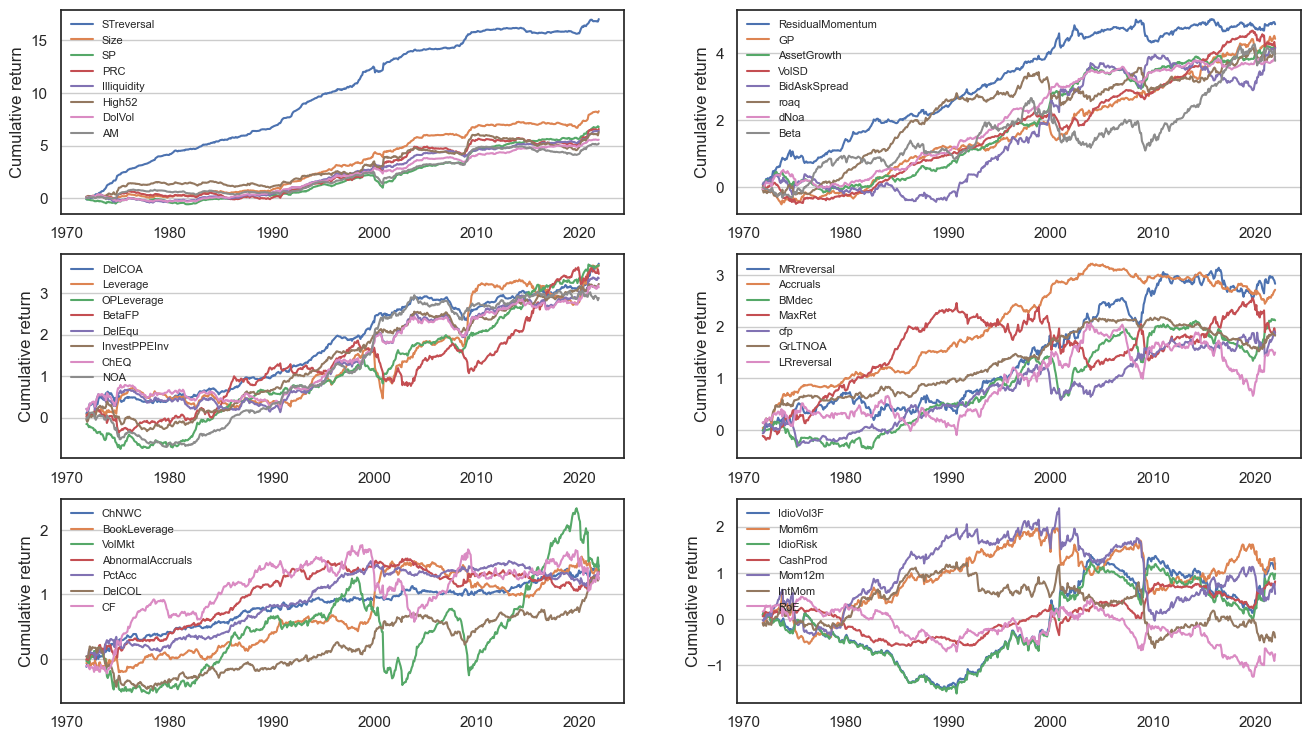
\includegraphics[width=.8\textwidth]{images/univariate_ls_cum_ret_ff3.png}
  \label{fig: ff3 univariate ls cumulative return}
  \caption*{\footnotesize{This graphic showcases firm characteristics sorted univariate long-short portfolios' cumulative return acrossing the whole time period, the return refering to the abnormal return derived from FF3 factor model.}}
\end{figure}

\begin{figure}[H]
  \centering
  \caption{\textbf{FF3 Abnormal Return: Univariate Long-short Portfolios Performance in Different Macroeconomic Conditions}}
  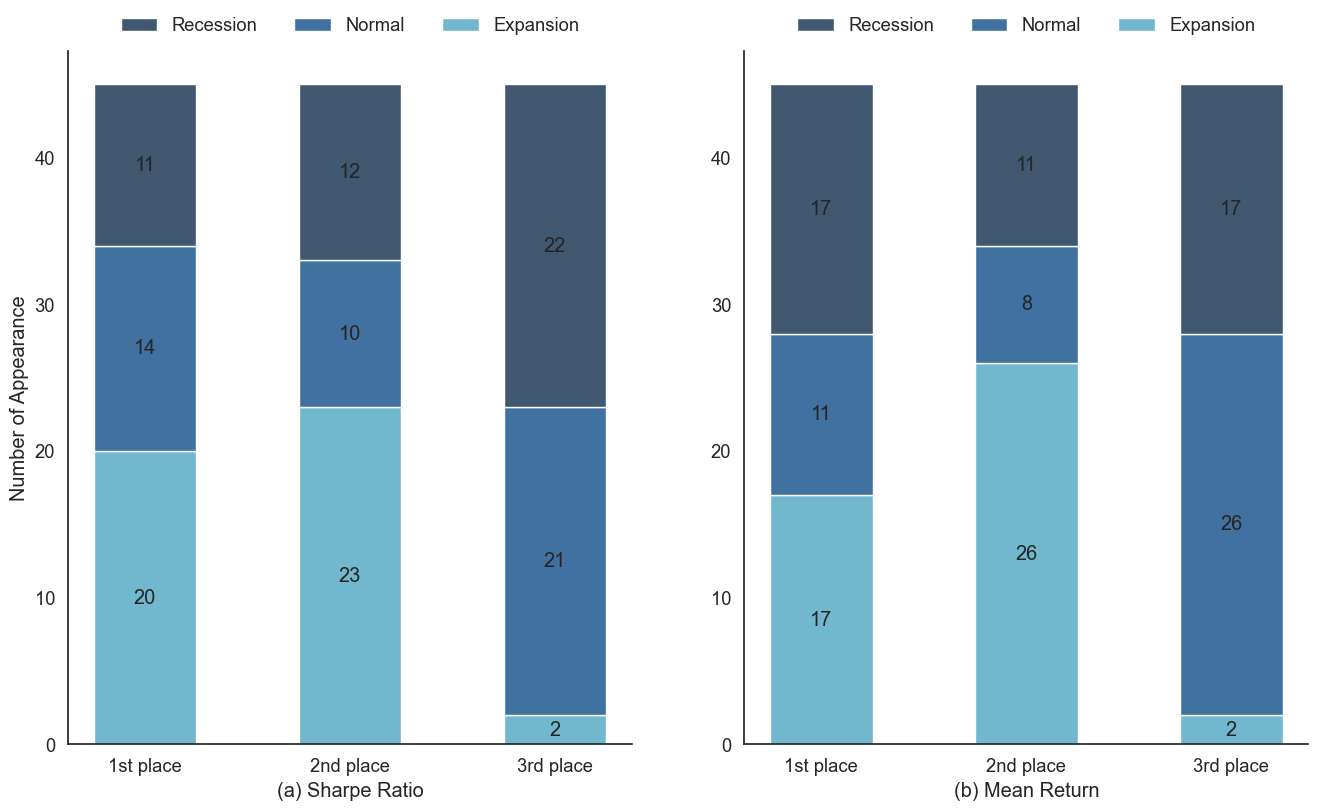
\includegraphics[width=.8\textwidth]{images/univariant_ls_ff3_comparing.png}
  \label{fig: ff3 univariate ls comparing}
  \caption*{\footnotesize{This graphic showcases firm characteristics sorted long-short univariate portfolios' performance across different macroeconomic conditions. We compare univariate long-short portfolios' sharpe ratio and mean return in recession, normal, and expansion periods, which is the horizontal comparision among the last 6 columns in table \ref{table: ff3 univariate ls portfolio}.}}
\end{figure}

\begin{table}[H]
  \centering
  \footnotesize
  \caption{\textbf{FF3 Abnormal Return: Univariate Long-short Portfolios' Returns}}
  \label{table: ff3 univariate ls portfolio}
  \begin{tabular}{lcc|cc|cc|cc}
  \hline
      ~ & \multicolumn{2}{c}{Full Sample} & \multicolumn{2}{c}{Recession} & \multicolumn{2}{c}{Normal} & \multicolumn{2}{c}{Expansion} \\
      ~ & SR & Mean & SR & Mean & SR & Mean & SR & Mean \\ \hline
      STreversal & 0.028 & 0.447 & 0.036 & 0.468 & 0.018 & 0.333 & 0.029 & 0.559 \\ 
      Size & 0.014 & 0.238 & 0.014 & 0.216 & 0.012 & 0.241 & 0.015 & 0.265 \\ 
      SP & 0.011 & 0.221 & 0.012 & 0.184 & 0.010 & 0.236 & 0.011 & 0.293 \\ 
      Illiquidity & 0.011 & 0.218 & 0.008 & 0.143 & 0.011 & 0.273 & 0.013 & 0.267 \\ 
      DolVol & 0.009 & 0.216 & 0.006 & 0.128 & 0.010 & 0.264 & 0.012 & 0.283 \\ 
      dNoa & 0.006 & 0.210 & 0.007 & 0.217 & 0.003 & 0.121 & 0.009 & 0.276 \\ 
      DelCOA & 0.006 & 0.202 & 0.006 & 0.189 & 0.003 & 0.120 & 0.009 & 0.274 \\ 
      VolSD & 0.007 & 0.191 & 0.001 & 0.037 & 0.011 & 0.354 & 0.009 & 0.235 \\ 
      GP & 0.007 & 0.184 & 0.005 & 0.118 & 0.011 & 0.258 & 0.007 & 0.183 \\ 
      AssetGrowth & 0.007 & 0.181 & 0.007 & 0.172 & 0.007 & 0.184 & 0.007 & 0.188 \\ 
      ResidualMomentum & 0.008 & 0.178 & 0.004 & 0.080 & 0.007 & 0.201 & 0.012 & 0.293 \\ 
      InvestPPEInv & 0.005 & 0.174 & 0.006 & 0.160 & 0.005 & 0.172 & 0.006 & 0.193 \\ 
      Accruals & 0.005 & 0.170 & 0.005 & 0.185 & 0.001 & 0.036 & 0.007 & 0.258 \\ 
      OPLeverage & 0.006 & 0.168 & 0.008 & 0.206 & 0.007 & 0.209 & 0.003 & 0.094 \\ 
      AM & 0.009 & 0.154 & 0.011 & 0.150 & 0.004 & 0.084 & 0.010 & 0.248 \\ 
      PRC & 0.011 & 0.149 & 0.018 & 0.207 & 0.006 & 0.087 & 0.009 & 0.132 \\ 
      DelEqu & 0.006 & 0.141 & 0.008 & 0.190 & 0.003 & 0.093 & 0.005 & 0.129 \\ 
      ChEQ & 0.005 & 0.136 & 0.009 & 0.198 & 0.001 & 0.044 & 0.005 & 0.137 \\ 
      NOA & 0.005 & 0.136 & 0.009 & 0.228 & 0.002 & 0.051 & 0.003 & 0.095 \\ 
      High52 & 0.010 & 0.133 & 0.022 & 0.222 & 0.000 & -0.006 & 0.008 & 0.136 \\ 
      roaq & 0.007 & 0.129 & 0.000 & 0.006 & 0.012 & 0.266 & 0.008 & 0.164 \\ 
      BetaFP & 0.006 & 0.124 & -0.003 & -0.060 & 0.012 & 0.314 & 0.009 & 0.217 \\ 
      Leverage & 0.006 & 0.121 & 0.007 & 0.104 & 0.002 & 0.040 & 0.009 & 0.247 \\ 
      GrLTNOA & 0.003 & 0.118 & 0.003 & 0.112 & 0.001 & 0.033 & 0.005 & 0.182 \\ 
      ChNWC & 0.002 & 0.113 & 0.005 & 0.216 & 0.000 & -0.021 & 0.003 & 0.114 \\ 
      BidAskSpread & 0.007 & 0.106 & 0.010 & 0.129 & 0.003 & 0.046 & 0.008 & 0.129 \\ 
      MRreversal & 0.005 & 0.097 & 0.008 & 0.139 & 0.001 & 0.025 & 0.005 & 0.106 \\ 
      BMdec & 0.004 & 0.096 & -0.003 & -0.079 & 0.005 & 0.127 & 0.009 & 0.300 \\ 
      AbnormalAccruals & 0.002 & 0.094 & 0.004 & 0.135 & -0.001 & -0.066 & 0.004 & 0.168 \\ 
      PctAcc & 0.002 & 0.093 & 0.001 & 0.043 & 0.001 & 0.050 & 0.004 & 0.181 \\ 
      Beta & 0.006 & 0.091 & 0.000 & 0.004 & 0.014 & 0.212 & 0.005 & 0.085 \\ 
      BookLeverage & 0.002 & 0.081 & 0.003 & 0.082 & 0.005 & 0.200 & 0.000 & -0.011 \\ 
      DelCOL & 0.002 & 0.077 & 0.002 & 0.054 & 0.002 & 0.101 & 0.002 & 0.081 \\ 
      cfp & 0.003 & 0.074 & -0.001 & -0.015 & 0.004 & 0.110 & 0.006 & 0.147 \\ 
      MaxRet & 0.003 & 0.057 & 0.001 & 0.009 & 0.004 & 0.096 & 0.005 & 0.091 \\ 
      LRreversal & 0.002 & 0.046 & 0.008 & 0.130 & -0.003 & -0.059 & 0.002 & 0.046 \\ 
      CF & 0.002 & 0.044 & -0.003 & -0.051 & 0.004 & 0.095 & 0.005 & 0.110 \\ 
      VolMkt & 0.002 & 0.043 & -0.008 & -0.121 & 0.008 & 0.212 & 0.007 & 0.142 \\ 
      CashProd & 0.001 & 0.043 & 0.000 & 0.012 & 0.000 & -0.012 & 0.004 & 0.150 \\ 
      IdioVol3F & 0.002 & 0.032 & 0.006 & 0.081 & -0.001 & -0.025 & 0.001 & 0.015 \\ 
      Mom6m & 0.002 & 0.028 & -0.005 & -0.064 & 0.006 & 0.108 & 0.005 & 0.096 \\ 
      IdioRisk & 0.002 & 0.026 & 0.006 & 0.082 & -0.002 & -0.030 & 0.000 & 0.001 \\ 
      Mom12m & 0.001 & 0.012 & -0.008 & -0.083 & 0.007 & 0.124 & 0.004 & 0.068 \\ 
      IntMom & -0.001 & -0.012 & -0.005 & -0.074 & 0.003 & 0.074 & 0.000 & 0.001 \\ 
      RoE & -0.001 & -0.025 & 0.006 & 0.103 & -0.006 & -0.141 & -0.004 & -0.078 \\ \hline
  \end{tabular}
  \begin{tablenotes}
    \footnotesize
    \item This table presents firm characteristics sorted univariate long-short portfolios' sharpe ratios and mean returns. The dataset has futher splitted into three different subsamples based on macroeconomic condition indicator -- CFNAI index, named by recession, normal, and expansion period. The return in this table refering to the abnormal stock return derived from FF3 factors model.
  \end{tablenotes}
\end{table}

\begin{figure}[H]
  \centering
  \caption{\textbf{Excess Return: Univariate Long-short Portfolios' Cumulative Return}}
  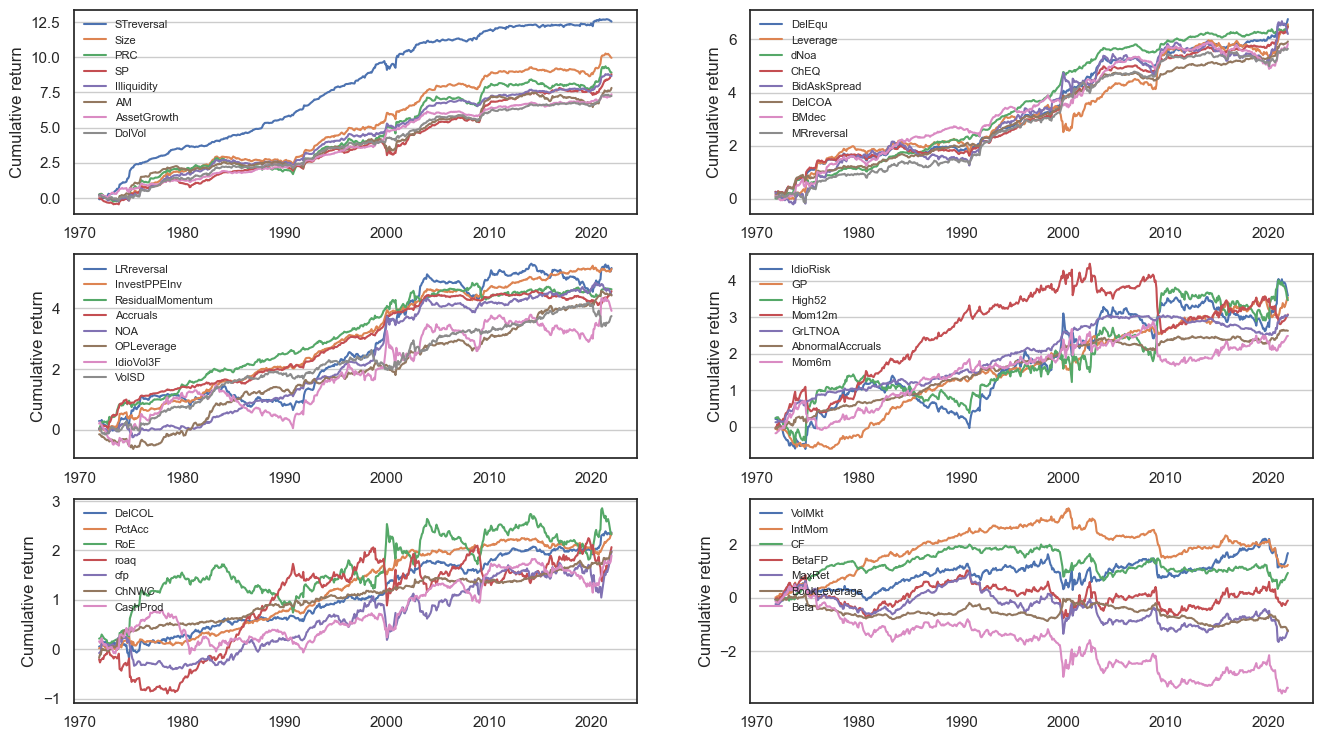
\includegraphics[width=.8\textwidth]{images/univariate_ls_cum_ret_excess.png}
  \label{fig: excess univariate ls cumulative return}
  \caption*{\footnotesize{This graphic showcases firm characteristics sorted univariate long-short portfolios' cumulative return acrossing the whole time period, the return refering to the stock excess return.}}
\end{figure}

\begin{figure}[H]
  \centering
  \caption{\textbf{Excess Return: Univariate Long-short Portfolios Performance in Different Macroeconomic Conditions}}
  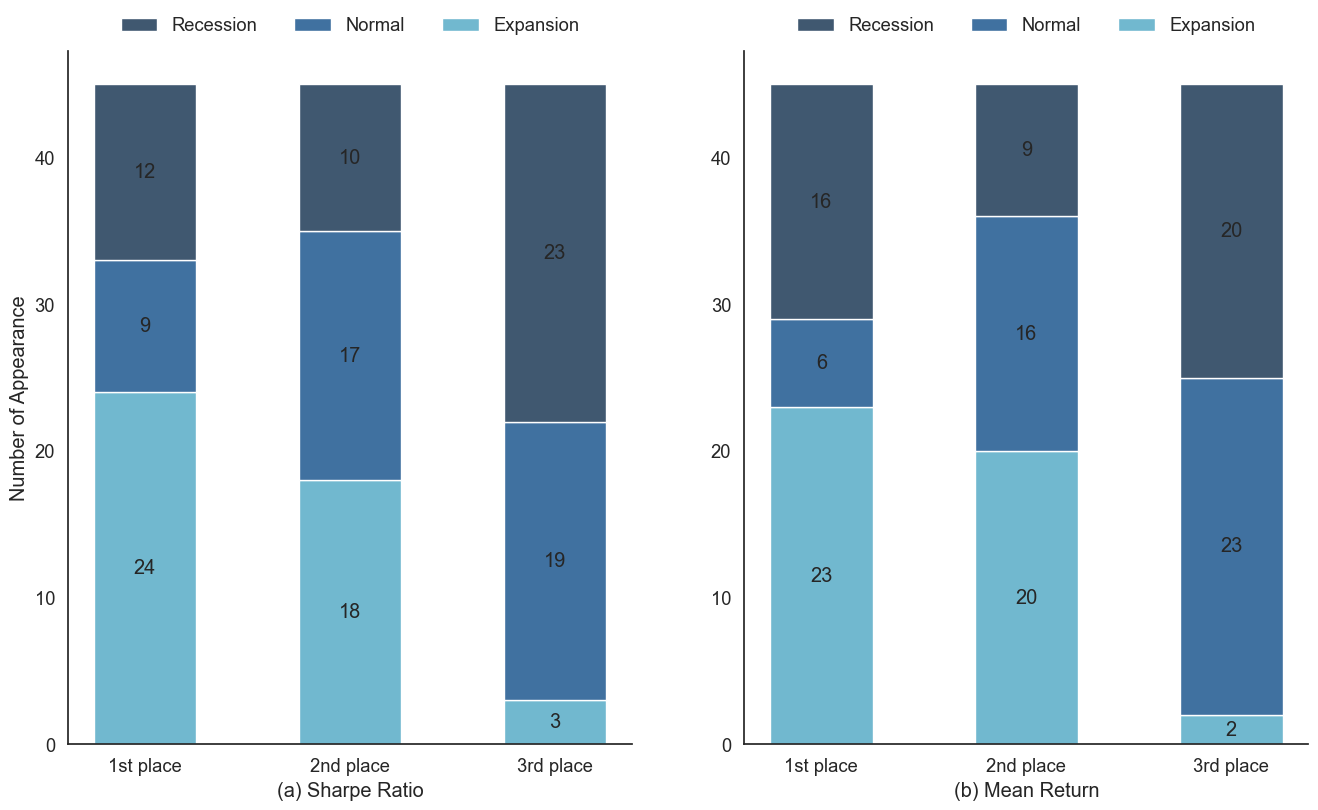
\includegraphics[width=.8\textwidth]{images/univariant_ls_excess_comparing.png}
  \label{fig: excess univariate ls comparing}
  \caption*{\footnotesize{This graphic showcases firm characteristics sorted long-short univariate portfolios' performance across different macroeconomic conditions. We compare univariate long-short portfolios' sharpe ratio and mean return in recession, normal, and expansion periods, which is the horizontal comparision among the last 6 columns in table \ref{table: excess univariate ls portfolio}.}}
\end{figure}

\begin{table}[H]
  \centering
  \footnotesize
  \caption{\textbf{Excess Return: Univariate Long-short Portfolios' Returns}}
  \label{table: excess univariate ls portfolio}
  \begin{tabular}{lcc|cc|cc|cc}
  \hline
      ~ & \multicolumn{2}{c}{Full Sample} & \multicolumn{2}{c}{Recession} & \multicolumn{2}{c}{Normal} & \multicolumn{2}{c}{Expansion} \\
      STreversal & 0.021 & 0.323 & 0.034 & 0.412 & 0.012 & 0.218 & 0.016 & 0.326 \\ 
      dNoa & 0.011 & 0.314 & 0.010 & 0.259 & 0.009 & 0.282 & 0.014 & 0.403 \\ 
      DelCOA & 0.010 & 0.296 & 0.009 & 0.246 & 0.007 & 0.256 & 0.014 & 0.377 \\ 
      AssetGrowth & 0.012 & 0.278 & 0.011 & 0.231 & 0.013 & 0.306 & 0.013 & 0.303 \\ 
      Accruals & 0.008 & 0.264 & 0.007 & 0.220 & 0.004 & 0.166 & 0.012 & 0.386 \\ 
      InvestPPEInv & 0.009 & 0.256 & 0.007 & 0.184 & 0.008 & 0.308 & 0.010 & 0.314 \\ 
      DelEqu & 0.011 & 0.253 & 0.012 & 0.253 & 0.009 & 0.243 & 0.012 & 0.262 \\ 
      ChEQ & 0.011 & 0.249 & 0.012 & 0.261 & 0.008 & 0.217 & 0.012 & 0.263 \\ 
      Size & 0.017 & 0.233 & 0.019 & 0.245 & 0.014 & 0.239 & 0.016 & 0.221 \\ 
      Illiquidity & 0.014 & 0.231 & 0.013 & 0.196 & 0.014 & 0.272 & 0.016 & 0.241 \\ 
      SP & 0.015 & 0.228 & 0.016 & 0.204 & 0.013 & 0.218 & 0.015 & 0.287 \\ 
      DolVol & 0.012 & 0.225 & 0.010 & 0.168 & 0.011 & 0.245 & 0.015 & 0.276 \\ 
      MRreversal & 0.009 & 0.193 & 0.014 & 0.244 & 0.004 & 0.087 & 0.010 & 0.220 \\ 
      OPLeverage & 0.007 & 0.193 & 0.009 & 0.220 & 0.008 & 0.235 & 0.005 & 0.128 \\ 
      BMdec & 0.010 & 0.192 & 0.002 & 0.042 & 0.012 & 0.270 & 0.015 & 0.318 \\ 
      GrLTNOA & 0.005 & 0.190 & 0.004 & 0.166 & 0.002 & 0.089 & 0.009 & 0.280 \\ 
      ResidualMomentum & 0.008 & 0.185 & 0.001 & 0.029 & 0.009 & 0.256 & 0.013 & 0.346 \\ 
      AM & 0.013 & 0.184 & 0.017 & 0.195 & 0.007 & 0.114 & 0.014 & 0.243 \\ 
      AbnormalAccruals & 0.004 & 0.178 & 0.005 & 0.200 & 0.001 & 0.065 & 0.006 & 0.237 \\ 
      NOA & 0.007 & 0.177 & 0.010 & 0.218 & 0.005 & 0.118 & 0.007 & 0.185 \\ 
      Leverage & 0.011 & 0.169 & 0.013 & 0.168 & 0.006 & 0.103 & 0.013 & 0.239 \\ 
      PRC & 0.015 & 0.169 & 0.024 & 0.230 & 0.008 & 0.124 & 0.011 & 0.135 \\ 
      PctAcc & 0.004 & 0.155 & 0.003 & 0.097 & 0.003 & 0.158 & 0.006 & 0.234 \\ 
      LRreversal & 0.009 & 0.149 & 0.013 & 0.194 & 0.006 & 0.119 & 0.008 & 0.125 \\ 
      ChNWC & 0.003 & 0.147 & 0.005 & 0.223 & 0.000 & 0.027 & 0.004 & 0.159 \\ 
      GP & 0.006 & 0.144 & 0.003 & 0.071 & 0.009 & 0.206 & 0.006 & 0.169 \\ 
      DelCOL & 0.004 & 0.135 & 0.003 & 0.085 & 0.005 & 0.197 & 0.004 & 0.145 \\ 
      BidAskSpread & 0.010 & 0.127 & 0.014 & 0.155 & 0.004 & 0.067 & 0.012 & 0.142 \\ 
      VolSD & 0.006 & 0.126 & 0.001 & 0.016 & 0.009 & 0.223 & 0.009 & 0.187 \\ 
      IdioVol3F & 0.007 & 0.076 & 0.012 & 0.124 & 0.003 & 0.045 & 0.004 & 0.047 \\ 
      CashProd & 0.003 & 0.074 & 0.003 & 0.054 & 0.001 & 0.028 & 0.005 & 0.139 \\ 
      IdioRisk & 0.006 & 0.071 & 0.012 & 0.122 & 0.003 & 0.039 & 0.003 & 0.039 \\ 
      Mom12m & 0.005 & 0.068 & -0.005 & -0.054 & 0.011 & 0.183 & 0.010 & 0.186 \\ 
      cfp & 0.003 & 0.065 & -0.001 & -0.026 & 0.005 & 0.114 & 0.006 & 0.134 \\ 
      RoE & 0.004 & 0.063 & 0.010 & 0.149 & -0.001 & -0.024 & 0.002 & 0.037 \\ 
      High52 & 0.006 & 0.062 & 0.024 & 0.193 & -0.006 & -0.089 & -0.002 & -0.026 \\ 
      Mom6m & 0.004 & 0.059 & -0.005 & -0.057 & 0.012 & 0.225 & 0.007 & 0.133 \\ 
      roaq & 0.003 & 0.055 & -0.003 & -0.040 & 0.010 & 0.175 & 0.004 & 0.072 \\ 
      IntMom & 0.002 & 0.039 & -0.004 & -0.066 & 0.004 & 0.088 & 0.006 & 0.140 \\ 
      VolMkt & 0.003 & 0.036 & -0.010 & -0.102 & 0.008 & 0.139 & 0.011 & 0.162 \\ 
      CF & 0.002 & 0.028 & -0.002 & -0.033 & 0.002 & 0.041 & 0.005 & 0.085 \\ 
      BetaFP & 0.000 & -0.002 & -0.011 & -0.110 & 0.004 & 0.066 & 0.007 & 0.104 \\ 
      MaxRet & -0.002 & -0.027 & -0.006 & -0.073 & -0.001 & -0.008 & 0.000 & 0.005 \\ 
      BookLeverage & -0.002 & -0.058 & -0.003 & -0.062 & 0.000 & -0.003 & -0.003 & -0.102 \\ 
      Beta & -0.006 & -0.066 & -0.013 & -0.126 & -0.003 & -0.037 & -0.001 & -0.013 \\ \hline
  \end{tabular}
  \begin{tablenotes}
    \footnotesize
    \item This table presents firm characteristics sorted univariate long-short portfolios' sharpe ratios and mean returns. The dataset has futher splitted into three different subsamples based on macroeconomic condition indicator -- CFNAI index, named by recession, normal, and expansion period. The return in this table refering to the stock excess return.
  \end{tablenotes}
\end{table}

%%%%%%%%%%%%%%%%%%%%%%%%%%%%%%%%%%%%%%%%%%%%%%%%%%%%%%%%%%%%%%%%%%%%%%%%%%%%%%%%%%%%%%%%
\subsection*{B2. Robust Result for Predictions Based Portfolios}\label{sec:appendixb2}

\begin{figure}[H]
  \centering
  \caption{\textbf{Cumulative Return of Portfolios Based on Prediction with Firm Features and CFNAI}}
  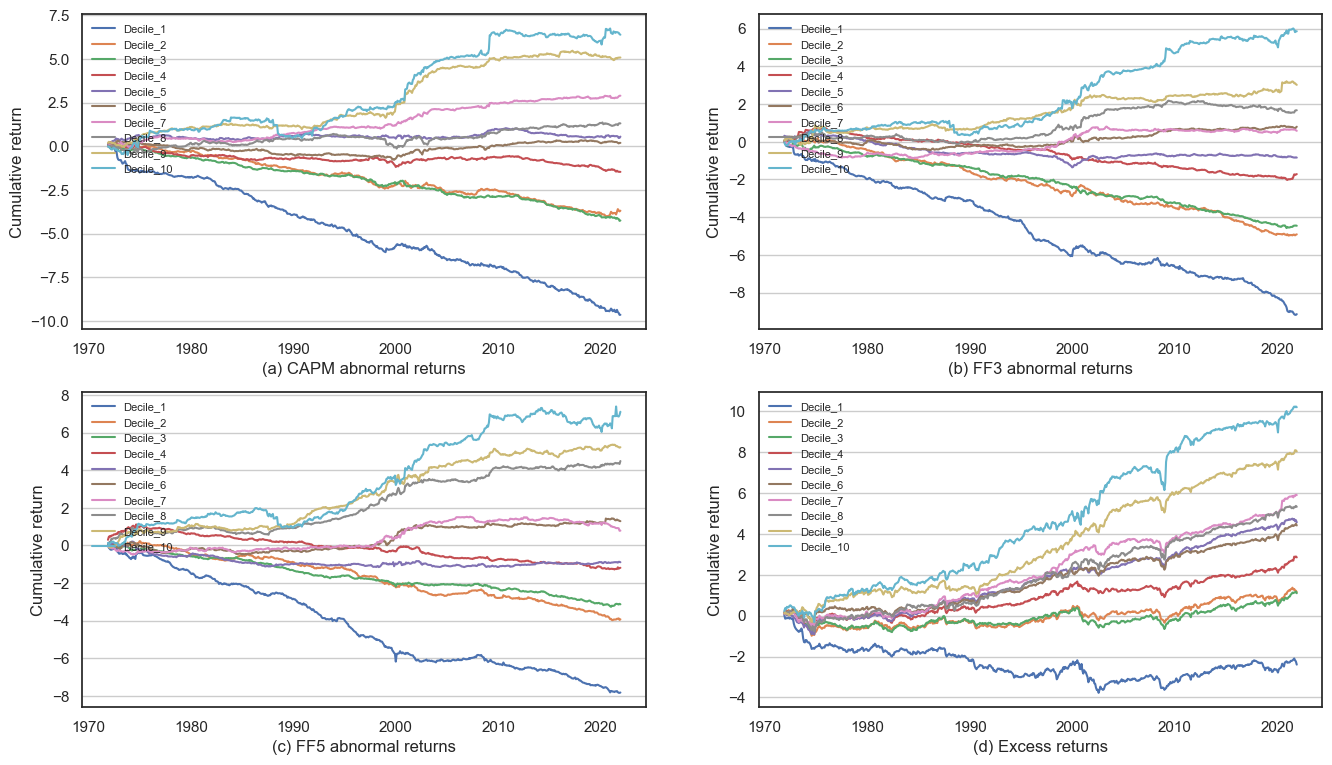
\includegraphics[width=.8\textwidth]{images/vw_portfolios_cumulative_return_cfnai.png}
  \label{fig: portfolios cum return firm features and cfnai}
  \caption*{\footnotesize{This graphic shows the cumulative return of value weighted portfolios based on predictions with firm characteristic feature variables and CFNAI data.}}
\end{figure}

\begin{figure}[H]
  \centering
  \caption{\textbf{Cumulative Return of Portfolios Based on Prediction with Firm Features and Sentiment}}
  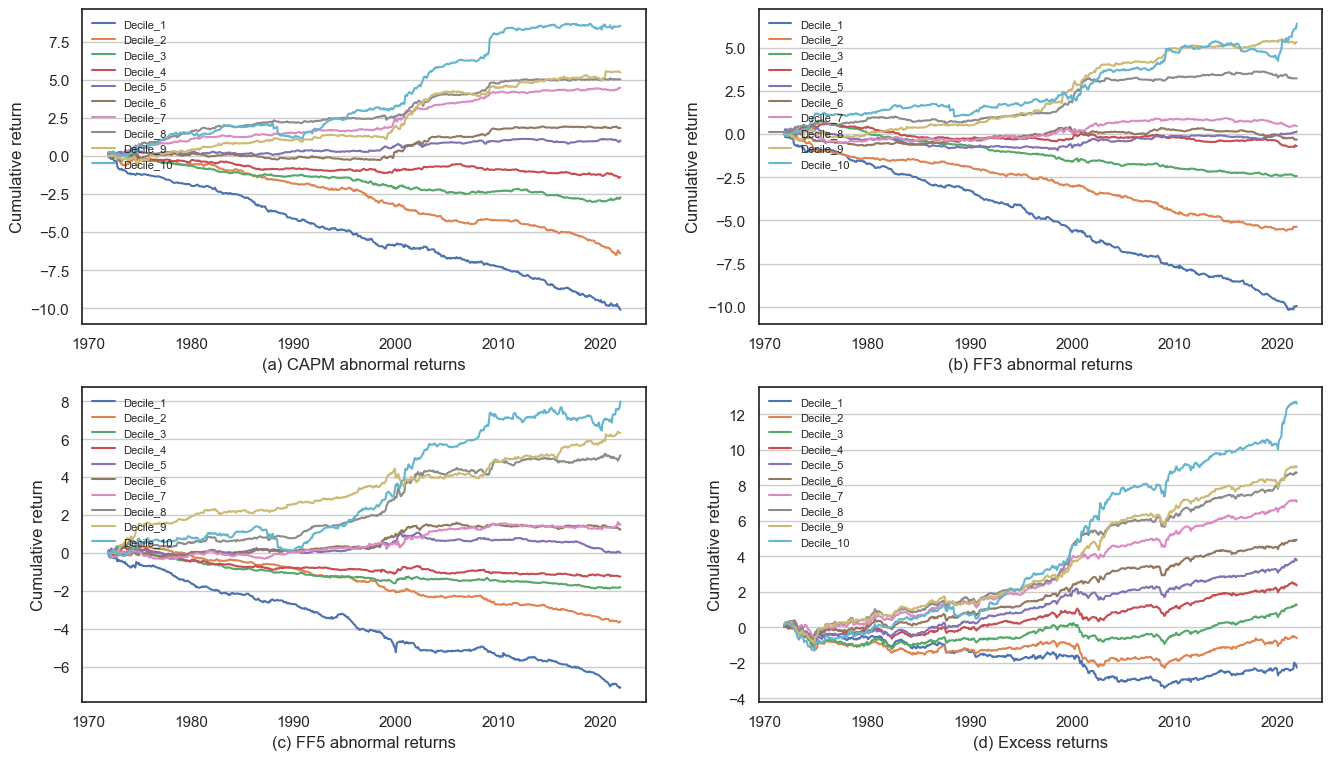
\includegraphics[width=.8\textwidth]{images/vw_portfolios_cumulative_return_sent.png}
  \label{fig: portfolios cum return firm features and sent}
  \caption*{\footnotesize{This graphic shows the cumulative return of value weighted portfolios based on predictions with firm characteristic feature variables and investors sentiment data.}}
\end{figure}

%%%%%%%%%%%%%%%%%%%%%%%%%%%%%%%%%%%%%%%%%%%%%%%%%%%%%%%%%%%%%%%%%%%%%%%%%%%%%%%%%%%%%%%%
\subsection*{B3. Robust Result for Feature Importance}
\label{sec:appendixb3}

\begin{figure}[H]
  \centering
  \caption{\textbf{Shap Feature Importance for CAPM Abnormal Return}}
  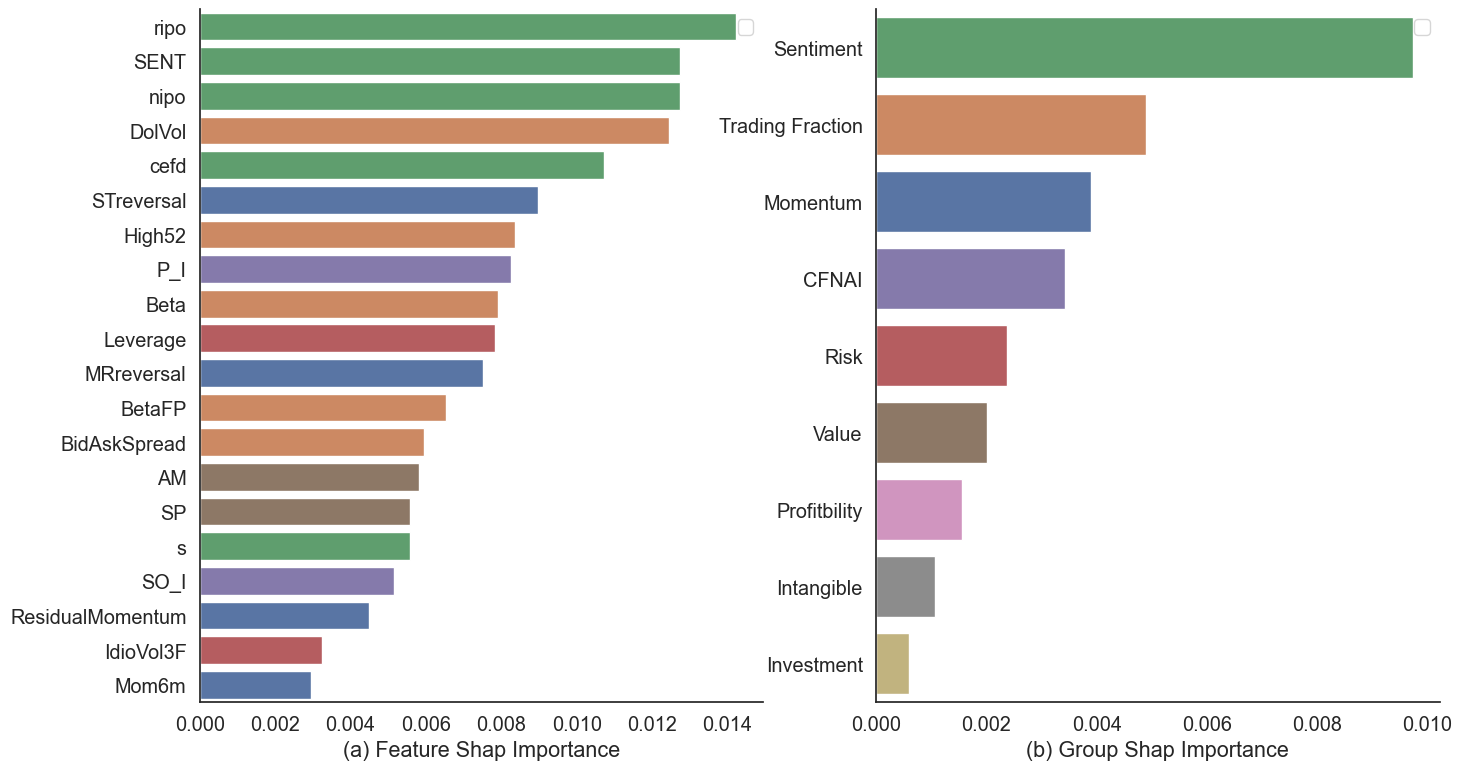
\includegraphics[width=.8\textwidth]{images/shap_feature_importance_capm.png}
  \label{fig: feature importance capm}
  \caption*{\footnotesize{This figure shows the importance ranking for predictor variables and variable groups in predicitng stock abnormal returns derived CAPM factor model. The ranking is the average of the feature variables' Shap force. The variable importance measures are evaluated on the testing dataset. Group shap importance is the feature importance's sum value within each group.}}
\end{figure}

\begin{figure}[H]
  \centering
  \caption{\textbf{Shap Feature Importance for FF3 Abnormal Return}}
  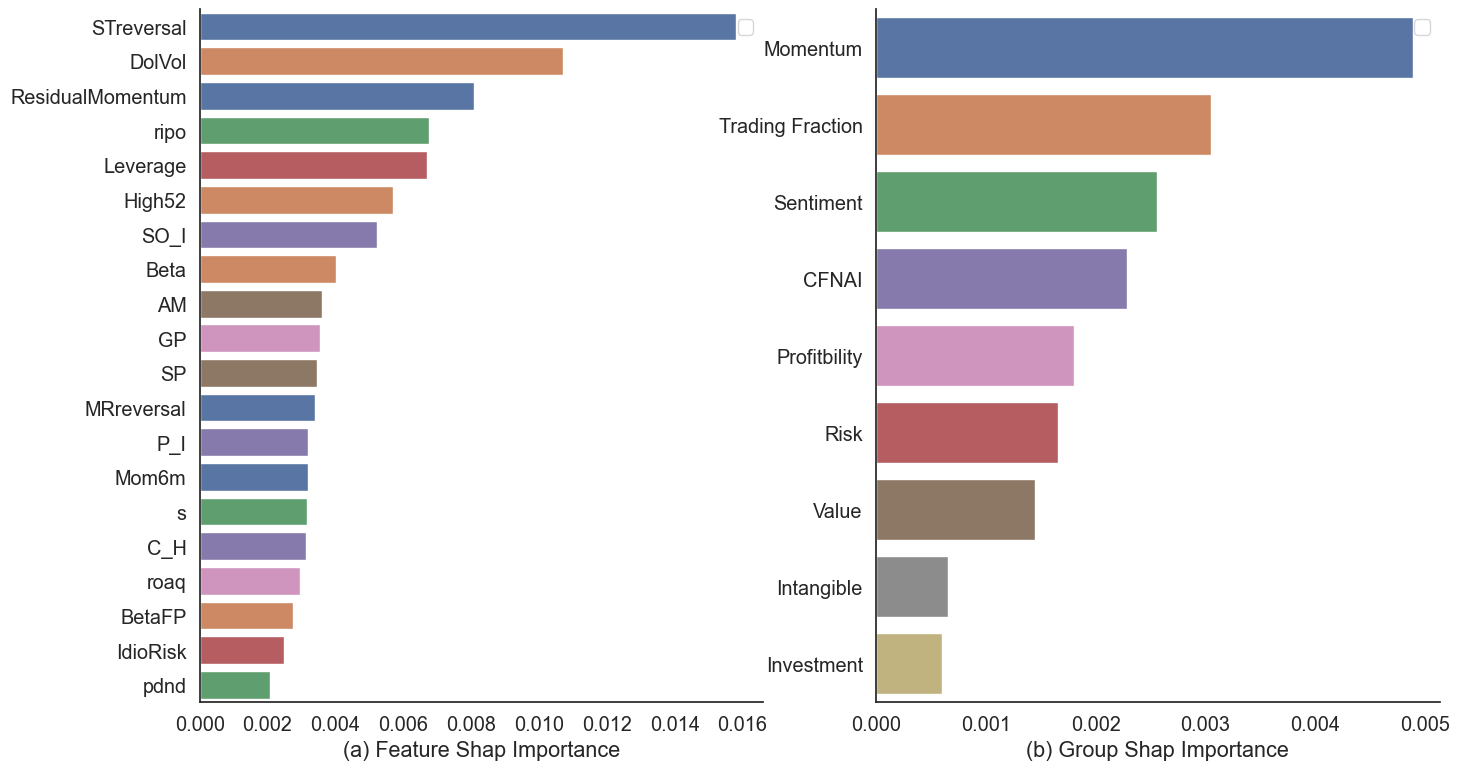
\includegraphics[width=.8\textwidth]{images/shap_feature_importance_ff3.png}
  \label{fig: feature importance ff3}
  \caption*{\footnotesize{This figure shows the importance ranking for predictor variables and variable groups in predicitng stock abnormal returns derived FF3 factors model. The ranking is the average of the feature variables' Shap force. The variable importance measures are evaluated on the testing dataset. Group shap importance is the feature importance's sum value within each group.}}
\end{figure}

%%%%%%%%%%%%%%%%%%%%%%%%%%%%%%%%%%%%%%%%%%%%%%%%%%%%%%%%%%%%%%%%%%%%%%%%%%%%%%%%%%%%%%%%
\subsection*{B4. Robust Result for Interaction Effects}
\label{sec:appendixb4}

\begin{figure}[H]
  \centering
  \caption{\textbf{Interaction Effects Between Firm Features and CFNAI, FF3}}
  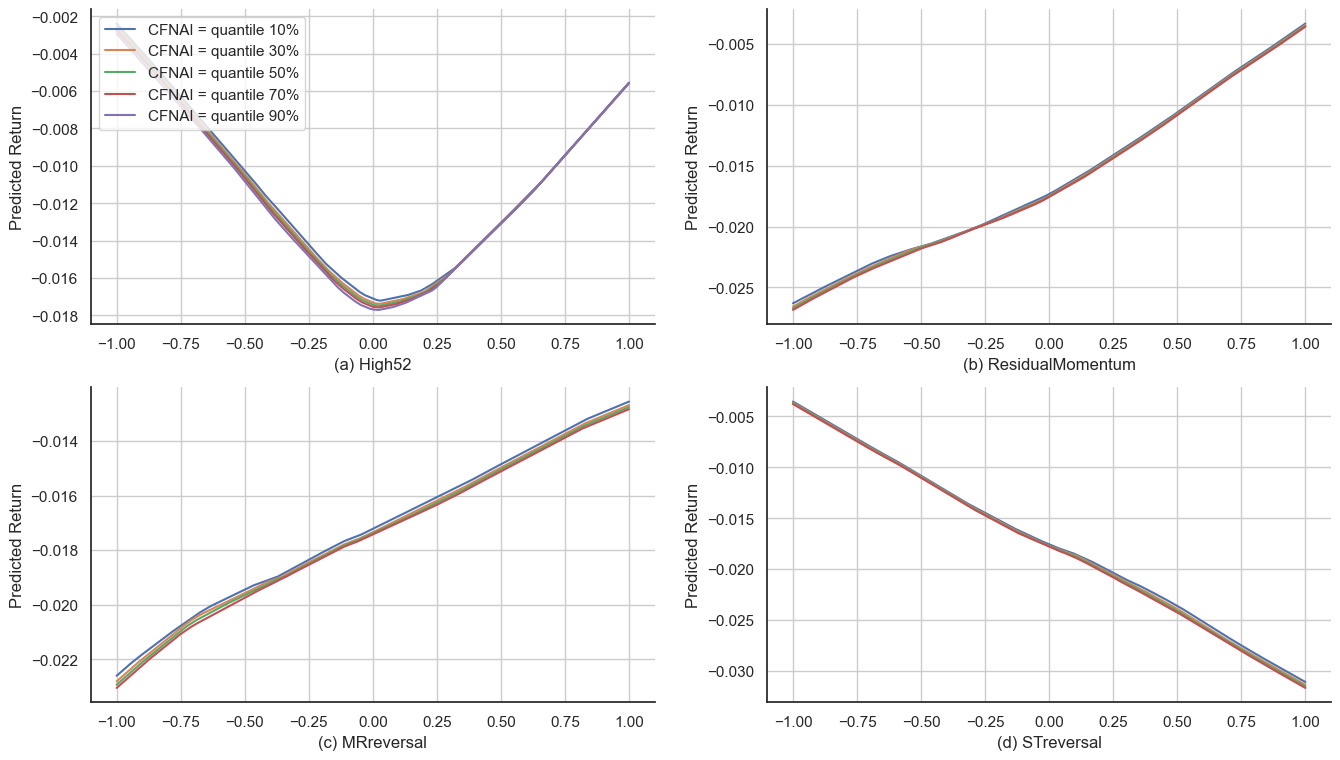
\includegraphics[width=.8\textwidth]{images/interactive_effect_ff3.png}
  \label{fig: interaction effect_ff3}
  \caption*{\footnotesize{This graphic shows the predicted stock abnormal return derived from FF3 factors model as a function of one stock characteristic feature variable, High52 (52 weeks trading high), ResidualMomentum (Momentum based on FF3 residuals  ), MRreversal (Medium‐run reversal), STreversal (Short term reversal) accordingly. The 'one' variable has a range between(-1, 1), macroeconomic variable CFNAI is seperated at 10\%, 30\%, 50\%, 70\%, and 90\% level. All other variables are fixed with the median value in the testing dataset.}}
\end{figure}

\begin{figure}[H]
  \centering
  \caption{\textbf{Interaction Effects Between Firm Features and CFNAI, CAPM}}
  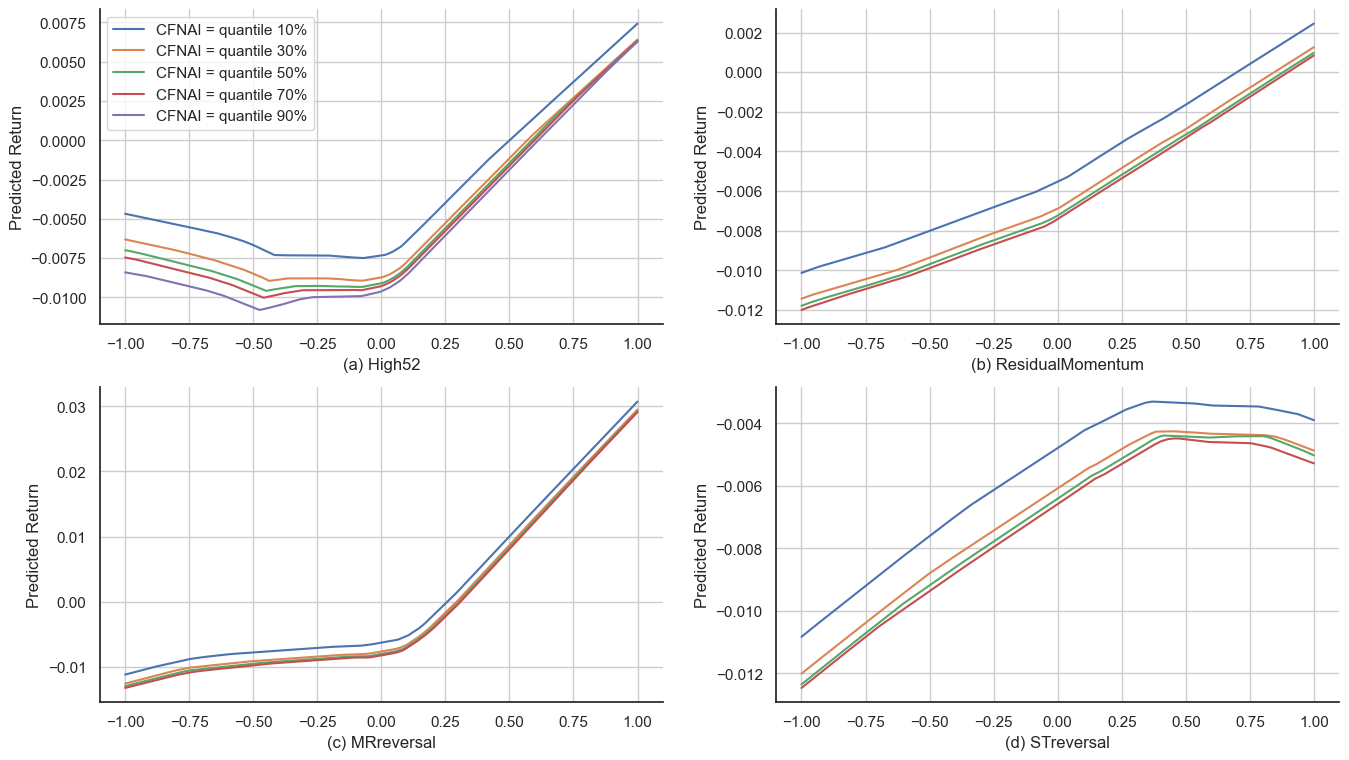
\includegraphics[width=.8\textwidth]{images/interactive_effect_capm.png}
  \label{fig: interaction effect_capm}
  \caption*{\footnotesize{This graphic shows the predicted stock abnormal return derived from CAPM model as a function of one stock characteristic feature variable, High52 (52 weeks trading high), ResidualMomentum (Momentum based on FF3 residuals  ), MRreversal (Medium‐run reversal), STreversal (Short term reversal) accordingly. The 'one' variable has a range between(-1, 1), macroeconomic variable CFNAI is seperated at 10\%, 30\%, 50\%, 70\%, and 90\% level. All other variables are fixed with the median value in the testing dataset.}}
\end{figure}

%%%%%%%%%%%%%%%%%%%%%%%%%%%%%%%%%%%%%%%%%%%%%%%%%%%%%%%%%%%%%%%%%%%%%%%%%%%%%%%%%%%%%%%%
\subsection*{B4. Robust Result for Market Timing}
\label{sec:appendixb5}

\begin{table}[H]
  \centering
  \caption{\textbf{Prediction Based Portfolios' Return in Defferent Macroeconomic Conditions}}
  \begin{tabular}{l|cc|cc|cc}
  \hline
      \multicolumn{7}{c}{(a) Portfolios' CAMP Abnormal Return (Mean)}\\\hline
      ~ & \multicolumn{2}{c}{Recession} & \multicolumn{2}{c}{Normal} & \multicolumn{2}{c}{Expansion} \\ \cline{2-7}
      Portfolios & Mean & Sharpe Ratio & Mean & Sharpe Ratio & Mean & Sharpe Ratio \\ \hline
      Decile\_1 & -1.503 & -0.338 & -1.263 & -0.275 & -1.035 & -0.195 \\ 
      Decile\_2 & -0.443 & -0.153 & -0.477 & -0.163 & -0.717 & -0.223 \\ 
      Decile\_3 & -0.333 & -0.123 & -0.252 & -0.113 & -0.463 & -0.145 \\ 
      Decile\_4 & -0.231 & -0.079 & -0.236 & -0.123 & -0.294 & -0.097 \\ 
      Decile\_5 & -0.111 & -0.035 & -0.050 & -0.024 & -0.273 & -0.087 \\ 
      Decile\_6 & 0.341 & 0.090 & 0.026 & 0.010 & -0.146 & -0.043 \\ 
      Decile\_7 & 0.443 & 0.121 & 0.156 & 0.057 & -0.220 & -0.065 \\ 
      Decile\_8 & 0.504 & 0.102 & 0.272 & 0.092 & 0.173 & 0.042 \\ 
      Decile\_9 & 1.331 & 0.238 & 0.616 & 0.176 & 0.438 & 0.091 \\ 
      Decile\_10 & 3.123 & 0.326 & 1.584 & 0.313 & 1.682 & 0.266 \\  \hline

      \multicolumn{7}{c}{(b) Portfolios' FF3 Abnormal Return (Mean)}\\\hline
      ~ & \multicolumn{2}{c}{Recession} & \multicolumn{2}{c}{Normal} & \multicolumn{2}{c}{Expansion} \\ \cline{2-7}
      Portfolios & Mean & Sharpe Ratio & Mean & Sharpe Ratio & Mean & Sharpe Ratio \\ \hline
      Decile\_1 & -1.778 & -0.397 & -1.642 & -0.533 & -1.485 & -0.382 \\ 
      Decile\_2 & -0.708 & -0.275 & -0.655 & -0.409 & -1.003 & -0.442 \\ 
      Decile\_3 & -0.656 & -0.301 & -0.371 & -0.261 & -0.564 & -0.237 \\ 
      Decile\_4 & -0.457 & -0.220 & -0.384 & -0.233 & -0.302 & -0.131 \\ 
      Decile\_5 & -0.334 & -0.143 & -0.200 & -0.123 & -0.200 & -0.084 \\ 
      Decile\_6 & 0.125 & 0.050 & -0.065 & -0.036 & -0.055 & -0.023 \\ 
      Decile\_7 & 0.168 & 0.061 & 0.120 & 0.061 & 0.003 & 0.002 \\ 
      Decile\_8 & 0.142 & 0.041 & 0.218 & 0.110 & 0.404 & 0.147 \\ 
      Decile\_9 & 1.021 & 0.243 & 0.616 & 0.205 & 0.784 & 0.244 \\ 
      Decile\_10 & 2.738 & 0.361 & 1.661 & 0.338 & 2.019 & 0.408 \\  \hline
  \end{tabular}
  \label{table: portfolio ret in tertiles rest}
  \begin{tablenotes}
    \footnotesize
    \item This table presents the actual mean portfolios' return and sharpe ratio in different macroeconomic conbinations. Portfolios are sorted based on the predicted abnormal and excess stock return made by neural network model. Macroeconomic conbinations defined as recession period, normal period, and expansion period based on the CFNAI index.
  \end{tablenotes}
\end{table}

\end{document}